\documentclass{llncs}
%\documentclass[11pt]{article}
\pagestyle{plain} 
\usepackage[operators,lambda,keys,sets,primitives,adversary,asymptotics,advantage]{cryptocode}
\usepackage{notations}
%\usepackage{bm}
\usepackage{mdframed}
\usepackage{enumitem}
%\usepackage{amsthm}
\usepackage{amsmath,amssymb}
\usepackage[utf8x]{inputenc}
\usepackage[colorinlistoftodos]{todonotes}
\usepackage{xspace}
\usepackage[normalem]{ulem}
\usepackage{comment}
\usepackage{multirow}
\usepackage[hidelinks]{hyperref}
\usepackage{url}
\newtheorem{assumption}{Assumption}
\newtheorem{fact}{Fact}
%\newtheorem{corollary}{Corollary}
\usepackage{etoolbox}
\patchcmd{\paragraph}{\itshape}{\bfseries\boldmath}{}{}

\begin{document}
\title{Transparent SNARKs from DARK Compilers}
\author{}
\institute{}
\author{Benedikt B\"unz\inst{1} \and Ben Fisch\inst{1} \and Alan Szepieniec\inst{2}}
\institute{Stanford \and Nervos Foundation}
\maketitle

\begin{abstract} 
We construct a new polynomial commitment scheme for univariate and multivariate polynomials over finite fields, with logarithmic size evaluation proofs and verification time, measured in the number of coefficients of the polynomial. The underlying technique is a \emph{Diophantine Argument of Knowledge} (DARK), leveraging integer representations of polynomials and groups of unknown order. Security is shown from the strong RSA and the adaptive root assumptions. Moreover, the scheme does not require a trusted setup if instantiated with class groups. We apply this new cryptographic compiler to a restricted class of algebraic linear IOPs, which we call \emph{Polynomial IOPs}, to obtain doubly-efficient public-coin interactive arguments of knowledge for any NP relation with succinct communication. With linear preprocessing, the online verifier's work is logarithmic in the circuit complexity of the relation.

There are many existing examples of Polynomial IOPs (PIOPs) dating back to the first PCP (BFLS, STOC'91). %Recently more efficient univariate PIOPs were presented in \textsf{Sonic} (MBKM, CCS'19), \textsf{PLONK} (GWC, ePrint'19), \textsf{Marlin} (CHM+, ePrint'19), \textsf{Fractal} (COS, TCC'19), and were also implicit in \textsf{STARKs} (BBHR, Crypto'19) and \textsf{Aurora} (BCR+, Eurocrypt'19). 
We present a generic compilation of any PIOP using our DARK polynomial commitment scheme. In particular, compiling the PIOP from \textsf{PLONK} (GWC, ePrint'19), an improvement on \textsf{Sonic} (MBKM, CCS'19), yields a public-coin interactive argument with quasi-linear preprocessing, quasi-linear (online) prover time, logarithmic communication, and logarithmic (online) verification time in the circuit size. Applying Fiat-Shamir results in a SNARK, which we call \textsf{\textbf{Supersonic}}. 

\textsf{Supersonic} is also concretely efficient with 10KB proofs and under $100$ms verification time for circuits with 1 million gates (estimated for 120-bit security). Most importantly, this SNARK is \emph{transparent}: it does not require a trusted setup. We obtain zk-SNARKs by applying a hiding variant of our polynomial commitment scheme with zero-knowledge evaluations. \textsf{Supersonic} is the first complete zk-SNARK system that has both a practical prover time as well as asymptotically \emph{logarithmic} proof size and verification time. 
\end{abstract} 

\section{Introduction}

Since the landmark discoveries of \emph{interactive proofs} (IPs)~\cite{STOC:GolMicRac85} and %the ``PCP theorem" on 
\emph{probabilistically checkable proofs} (PCPs)~\cite{STOC:BFLS91,FOCS:ALMSS92} in the 90s, there has been tremendous development in the area of proof systems whereby a prover establishes the correct performance of an arbitrary computation in a way that can be verified much more efficiently than performing the computation itself. Such proof systems are \emph{succinct} if they also involve induce a low communication cost between the prover and the verifier, \emph{i.e.}, the transcript of the protocol is much smaller than a witness to the computation. There are also \emph{zero knowledge} variants of these efficient proof systems, beginning with ZK-IPs~\cite{C:BGGHKMR88} and ZK-PCPs~\cite{STOC:Kilian92}, in which the computation may involve secret information and the prover demonstrates correct performance without leaking the secrets. As a toy example, one could prove that a chess position is winning for white without actually revealing the winning moves themselves. General purpose zero-knowledge proofs~\cite{JACM:GMW91} can be very expensive in terms of proof size and verification time even for computations that would be easy to perform given the secret inputs (\emph{e.g.}, by proving that one decrypted a file properly without leaking the key or the plaintext). The same techniques that are used to build efficient proof systems for expensive computations are also useful for making zero-knowledge proofs more practical. 
%A more practical example  
 
In recent years, there has been a surge of industry interest in verifiable outsourced computation~\cite{WalBlu15} (such as trustless cloud computing) as well as zero-knowledge proofs. In particular, blockchains use efficient zero-knowledge proofs as a solution for balancing privacy and publicly-verifiable integrity: examples include anonymous transactions in ZCash~\cite{SP:BCGGMT14,Zcash} and verifying Ethereum smart contracts over private inputs~\cite{Zokrates}. In these applications, zero-knowledge proofs are posted to the blockchain ledger as a part of transactions and nodes must verify many proofs in the span of a short period of time. Therefore, succinctness and fast verification are necessary properties for the deployment of such proof systems. Verifiable computation is also being explored as a scaling solution for blockhain transactions~\cite{ZK-rollup}, and even as a way to entirely eliminate the need for maintaining historical blockchain data~\cite{Coda}. 
%In recent years, there has been a surge of industry interest in applying proof systems to outsourced verifiable computation~\cite{Sources}. These proof systems are particularly relevant to blockchains, which use efficient zero-knowledge proofs as a solution for balancing privacy and publicly-verifiable integrity: examples include anonymous transaction in ZCash~\cite{SP:BCGGMT14,Zcash}, and verifying Ethereum smart contracts over private inputs~\cite{ZKContracts}. Verifiable computation is also used as a way to synchronize more efficiently with the current state of a blockchain~\cite{Rollup}, or even entirely eliminate the need for maintaining historical blockchain data~\cite{Coda}. 

Following this pragmatic interest, there has also been a surge of research focused on obtaining proof systems with better concrete efficiency characteristics: \emph{succinctness} (the proof size is sublinear in the original computation length $T$), \emph{non-interactivity} (the proof is a single message), \emph{prover-scalability} (proof generation time scales linearly or quasi-linearly in $T$), and \emph{verifier-scalability} (verification time is sublinear in $T$). Proof systems that achieve all of these properties for general NP statements%\footnote{NP statements can be verified deterministically in polynomial time given a suitable \emph{witness}. More formally, a language $L \subseteq \{0,1\}^*$ is in $NP$ if there is a non-determinstic polynomial time decision algorithm $V_L$ for $L$: for every $x \in \{0,1\}^*$ there exists a witness $w$ such that $V_L(x, w) = 1$ iff $x \in L$. If $C$ is a circuit, the statement that $C(x) = y$ can be expressed as an NP statement $(C, x, y)$ with a witness $w$ that assigns correct values to all the internal wires of $C$ producing the output $y$ on input $x$.}
are called SNARGs (``succinct non-interactive arguments''). 
The proof is called an \emph{argument} when it is only sound assuming the prover is computationally bounded, \emph{i.e.}, \emph{computationally sound} as opposed to statistically sound. 
Succinct statistically sound proofs are unlikely to exist~\cite{CC:GolVadWig02,ICALP:Wee05}.

Currently, there are numerous constructions that achieve different tradeoffs between proof size, proof time, and verification time, but also under different \emph{trust} models as well as cryptographic assumptions. %There is a distinction between \emph{proofs} and \emph{arguments}, the latter offering soundness only against a computationally bounded prover. 
Some constructions also achieve better efficiency by relying on a \emph{preprocessing model} in which a one-time expensive setup procedure is performed in order to generate a compact verification key \pro{VK}, which is later used to verify proof instances efficiently.
%More precisely, a fresh \pro{VK} must be generated for each computation that will be proven, e.g. represented as an arithmetic circuit $C$ that takes inputs $x \in \ZZ^n$ over a prime field $\ZZ$. Thereafter, succinct proofs may be generated for the evaluation of $C$ on arbitrary inputs $x$ and verified efficiently with \pro{VK}. 
Somewhat unfortunately, the best performing proof systems to date (considering proof size and verification time) require a \emph{trusted} preprocessing. These are the pairing-based SNARKs extending from GGPR~\cite{EC:GGPR13,ES:SBVBPW13,TCC:BCIOP13,C:BCGTV13,EC:Groth16}, which have been implemented in numerous libraries~\cite{C:BCGTV13,bellman}, and even deployed in live systems such as the ZCash~\cite{Zcash} cryptocurrency.
%The preprocessing involves secret information that must be discarded, else it provides the prover with a trapdoor that breaks the integrity of the proof system. 
The trusted setup can be performed via \emph{multi-party computation} (MPC) by a committee of parties, such that trust in only one of the parties is sufficient. This has been done on two occasions for the ZCash blockchain, involving elaborate ``ceremonies" to engender public trust in the process~\cite{ZcashCeremony}. 

A proof system is called \emph{transparent} if it does not involve any trusted setup. Recent progress has yielded transparent proof systems for special types of computations: zk-\textsf{STARK}s~\cite{C:BBHR19} generate zero-knowledge proofs of size $O(\lambda \log^2 T)$ for a uniform computation\footnote{A uniform computation is expressed as a RAM program $P$ and a time bound $T$ on the running time of the program. While the size of $P$'s description does affect the proof size, the clue is that the size of this description does not scale with the time bound $T$.}, and the GKR protocol produces interactive proofs with communication $O(d \log T)$ for computations expressed as low-depth circuits of total size $T$ and depth $d$~\cite{STOC:GolKalRot08}. In both cases, non-interactivity can be achieved in the random oracle model with the Fiat-Shamir heuristic~\cite{C:FiaSha86,STOC:CCHLRRW19}.
These transparent proof systems perform significantly worse than SNARKs based on preprocessing. For computations expressed as an arithmetic circuit of $1$-million gates, \textsf{STARK}s~\cite{C:BBHR19} report a proof size of $600$KB, whereas preprocessing SNARKs achieve $200$ bytes~\cite{EC:Groth16}. Bulletproofs~\cite{SP:BBBPWM18, EPRINT:BCCGP16} is a transparent zero-knowledge proof system whose proofs are much smaller than those of \textsf{STARK}, but these proofs have a verification time that scales linearly in the size of the circuit; for an arithmetic circuit of one million gates the verification time is close to 1 minute, more than 1,000 times more expensive than verifying a \textsf{STARK} proof for the same computation. 
% The original GKR protocol was not zero-knowledge, but there are more recent zero-knowledge variants that have communication $O( \sqrt{n} + d \log T)$ where $n$ is the size of the (secret) input~\cite{SP:WTSTW18,EPRINT:ZGKPP17b}. 


Another thread of research has produced proof systems that remove trust from the circuit preprocessing step, and instead have a \emph{universal} (trusted) setup: a one-time trusted setup that can be reused for \emph{any} computation~\cite{Sonic,Libra,Spartan,Plonk}. All of these systems build SNARKs by combining an underlying reduction of circuit satisfiability to probabilistic testing of polynomials (with degree at most linear in the circuit size) together with \emph{polynomial commitment schemes}. In a polynomial commitment scheme, a prover commits to a $\mu$-variate polynomial $f$ over $\FF$ of degree at most $d$ with a message that is much smaller than sending all the coefficients of $f$. The prover can later produce a non-interactive argument that $f(z) = y$ for arbitrary $z \in \FF^\mu$ and $y \in \FF$. %It should be infeasible for the prover to claim $f(z) = y'$ and $f(z) = y$ for $y \neq y'$. Universal SNARK constructions also require this evaluation protocol to itself be a knowledge argument, \emph{i.e.}, a successful prover must know the coefficients of the committed polynomial. 
The trusted portion of the universal SNARK is entirely confined to the polynomial commitment scheme's setup. These constructions use variants of the Kate~\emph{et al.} commitment scheme for univariate polynomials~\cite{AC:KatZavGol10}, which requires a trusted setup.% trusted party to generate a length $d$ vector of group elements of the form $g^{s^i}$ for a secret point $s \in \FF$. 

%According to a concrete comparison~\cite{Libra} of proof systems' performance (prior to the present work) on a computation that derives the root of a SHA-256 Merkle tree with 256 leaves\footnote{This computation involves 511 calls to SHA-256.}, STARKs are the only transparent non-interactive proof system capable of producing a proof (in a practical\footnote{The STARK computation cited here takes about 30 minutes to generate.}  amount of time) that can be verified in under 9 seconds, and yet the proof size is nearly 400 KB. 

\subsection{Summary of contributions} 
Following the observations of the recent universal SNARK constructions~\cite{Plonk,Sonic,Libra}, SNARKs can be built from polynomial commitment schemes where all the trust is confined to the setup of the commitment scheme. The main technical contribution of our work is thus a new polynomial commitment scheme without trusted setup (\emph{i.e.}, a transparent polynomial commitment scheme), which we can use to construct transparent SNARKs. The observation that transparent polynomial commitments imply transparent SNARKs was also implicit in the recent works that build transparent SNARKs from multi-round classical PCPs, and specifically interactive oracle proofs of proximity (IOPPs)~\cite{ICALP:BBHR18}. As a secondary contribution, we present a framework that unifies all existing approaches to constructing SNARKs from polynomial commitments using the language of \emph{interactive oracle proofs} (IOPs)~\cite{STOC:ReiRotRot16,TCC:BenChiSpo16}. We view polynomial commitment schemes as a compiler for \emph{Polynomial IOPs}, and re-characterize the results of prior works as providing a variety of Polynomial IOPs for NP. 

\paragraph{New polynomial commitment scheme} We construct a new polynomial commitment scheme for $\mu$-multivariate polynomials of degree $d$ with optional zero-knowledge arguments of knowledge for correct evaluation that have $O(\mu \log d)$ size proofs and are verifiable in $O(\mu \log d)$ time. The commitment scheme requires a group of unknown order: two candidate instantiations are RSA groups and class groups of an imaginary quadratic order. Using RSA groups, we can apply the scheme to obtain universal preprocessing SNARKs with \emph{constant-size} %\footnote{The security parameters are technically size $O(\lambda)$ where $\lambda$ is a security parameter.}
setup parameters, as opposed to the linear-size parameters from previous attempts. Using class groups, we can remove the trusted setup from trusted-setup SNARKs altogether, thereby making them \emph{transparent}. Our polynomial commitment scheme leverages the power of integer commitments and \emph{Diophantine Arguments of Knowledge}~\cite{AC:Lipmaa03a}; accordingly, we classify this tool (and others of its kind) as a \emph{DARK} proof system.
%obtain the first transparent SNARKs with $O(\log d)$ proof size and $O(\log d)$ verification time.

\paragraph{Polynomial IOP formalism} %As a secondary contribution, we present a framework that unifies all existing approaches to constructing SNARKs from polynomial commitments. This framework is based on interactive oracle proofs
All SNARK constructions can be viewed as combining an underlying information-theoretic statistically-sound protocol with a ``cryptographic compiler'' that transforms the underlying protocol into a succinct argument at the cost of computational soundness. 
We define a \emph{Polynomial IOP} as a refinement of algebraic linear IOPs~\cite{CC:IKO07,TCC:BCIOP13,C:BBCGI19}, where in each round of interaction the prover provides the verifier with oracle access to a multivariate polynomial function of bounded degree. The verifier may then query this oracle to evaluate the polynomial on arbitrary points of its choice. The existing universal and transparent SNARK constructions provide a variety of statistically-sound Polynomial IOPs for circuit satisfiability (or RAM programs, in the case of \textsf{STARK}s); these are then cryptographically compiled using some form of a polynomial commitment, typically using Merkle trees or pairing groups.

The linear PCPs underlying GGPR and its successors (\emph{i.e.}, based on QAPs and R1CS) can also be transformed into Polynomial IOPs.\footnote{This observation was also implicit in the paper by Ben-Sasson \emph{et al.} introducing the system \pro{Aurora}~\cite{EC:BCRSVW19}.} This transformation helps highlight the fundamental paradigm shift between constructions of non-transparent non-universal SNARKs that combine linear PCPs and \emph{linear-only encodings} versus the more recent ones based on polynomial commitments: given the lack of efficient\footnote{Lai and Malavota~\cite{C:LaiMal19} provide a $n$-dimensional \emph{linear-map} commitment based on bilinear pairings, extending techniques in functional commitments~\cite{ICALP:LibRamYun16}, but verifying claimed evaluations of the committed function on query points takes $O(n)$.} \emph{linear function} commitment schemes, the compilation of linear PCPs \emph{necessarily} involves a trusted preprocessing step that preselects the verifier's linear PCP queries, and hides them inside a linear-only encoding. This linear-only encoding forces the prover to homomorphically output an (encoded) linear tranformation of the query, upon which the verifer performs several homomorphic checks (\emph{e.g.}, using pairings).
The shift towards Polynomial IOPs, which can be compiled more directly with efficient polynomial commitments, avoids the involvement of a trusted party to place hidden queries in the preprocessing. The only potential need for non-transparent setup is in the instantiation of polynomial commitment itself.

The precise definition of Polynomial IOPs as a central and standalone notion raises the question about its exact relation to other IOP notions. We present a univariate Polynomial IOP for extracting an indicated coefficient of a polynomial. 
%This construction establishes that adding point queries to univariate Polynomial IOPs does not make them more powerful. 
Furthermore, we present a univariate Polynomial IOP for proving that the inner product between the coefficient vectors of two polynomials equals a given value. This proof system is of independent interest. Together with an offline pre-processing phase during which the correctness of a multivariate polynomial is ascertained, these two tools enable us to show that \emph{any} algebraic linear IOP can be realized with a multivariate Polynomial IOP. 



\paragraph{Polynomial IOP compiler} 
We present a generic compilation of any public-coin Polynomial IOP into a doubly-efficient public-coin interactive argument of knowledge using an abstract polynomial commitment scheme. We prove that if the commitment scheme's evaluation protocol has witness-extended emulation, then the compiled interactive argument has this knowledge property as well. If the commitment scheme is hiding and the evaluation is honest-verifier zero knowledge (HVZK), then the compiled interactive argument is HVZK as well. Finally, public-coin interactive arguments may be cryptographically compiled into SNARKs using the Fiat-Shamir heuristic.\footnote{Security for Fiat-Shamir has been proven secure in the random oracle model for constant-round protocols, for multi-round protocols satisfying \emph{soundness against restoration attacks}, and in some cases using correlation-intractable hash functions~\cite{C:FiaSha86,TCC:BenChiSpo16,C:KalRotRot17,EC:CCRR18,STOC:CCHLRRW19}.}
%\cite{C:FiaSha86,CCS:BelRog93,EC:PoiSte96,CSproofs,TCC:HalMyeRac08,TCC:BenChiSpo16,EC:AABN02,C:KalRotRot17,EC:CCRR18,FOCS:HolLom18,STOC:CCHLRRW19}.}

\paragraph{New SNARK without Trusted Setup}
The main practical outcome of this work is a new transparent proof system (\pro{Supersonic}) for computations represented as arbitrary arithmetic circuits, obtained by cryptographically compiling the Polynomial IOPs underlying \textsf{Sonic}~\cite{Sonic} and \textsf{PLONK}~\cite{Plonk} using the DARK polynomial commitment scheme. \pro{Supersonic} improves the proof size by an order of magnitude over \textsf{STARK}s without compromising on verification time. For one million gates, \pro{Supersonic}'s proofs are just 7.8KB and take around 75ms to verify. 
As a caveat, while the prover time in \pro{Supersonic} is asymptotically on par with \textsf{STARK}s (\emph{i.e.}, quasilinear in $T$), the concrete efficiency is much worse due to the use of heavy-weight ``crypto operations'' over 1200 bit class group elements in contrast to the light-weight FFTs and hash functions in \textsf{STARK}s. Furthermore, \pro{Supersonic} is not quantum-secure due to its reliance on groups of unknown order, whereas \textsf{STARK}s are a candidate quantum-secure SNARK. 

\subsection{Related Work}

\paragraph{Arguments based on hidden order groups} 
Fujisaki and Okamoto~\cite{C:FujOka97} proposed homomorphic integer commitment schemes based on the RSA group. They also provide protocols to prove that a list of committed integers satisfy modular polynomial equations as opening a commitment bit by bit. Damgård and Fujisaki~\cite{AC:DamFuj02} patched the soundness proof of that protocol and were the first to suggest using class groups of an imaginary quadratic order as a candidate group of unknown order. Lipmaa drew the link between zero-knowledge proofs constructed from integer commitment schemes and Diophantine complexity~\cite{AC:Lipmaa03a}, coining the term \emph{Diophantine Arguments of Knowledge}. Recently, Couteau~\emph{et al.} study protocols derived from integer commitments specifically in the RSA group to reduce the security assumptions needed; in the process they develop proofs for polynomial evaluation modulo a prime $\pi$ that is not initially known to the verifier, in addition to a proof showing that an integer $X$ lies in the range $[a,b]$ by showing that $1+4(X-a)(b-X)$ decomposes as the sum of 3 squares~\cite{EC:CouPetPoi17}.

Pietrzak~\cite{ITCS:Pietrzak18} developed an efficient proof of repeated squaring, \emph{i.e.}, proving that $x^{2^T} = y$ with $O(\log T)$ proof size and verification time in order to build a conceptually simple verifiable delay function~\cite{C:BBBF18} based on the RSW time-lock puzzle~\cite{RivShaWag96}. Wesolowski~\cite{EC:Wesolowski19} improves on this result by proposing a single-round protocol to prove correct repeated squaring in groups of unknown order with a constant size proof. Boneh~\emph{et al.}~\cite{C:BonBunFis19} observe that this protocol generalizes to arbitrary exponents (PoE) and develop a proof of knowledge of an integer exponent (PoKE), as well as a zero-knowledge variant. They apply both PoE and PoKE to constructing efficient accumulators and vector commitment schemes.

\paragraph{Transparent polynomial commitments} 
Whaby \emph{et al.} constructed a transparent polynomial commitment scheme~\cite{SP:WTSTW18} combining a matrix commitment of Bootle~\emph{et al.}~\cite{EC:BCCGP16} with the inner-product argument of B\"{u}nz~\emph{et al.}~\cite{SP:BBBPWM18}. This commitment works for multilinear polynomials. For polynomials of degree $d$ it has $O(\sqrt{d})$ size commitments and evaluation arguments with $O(\sqrt{d})$ communication. 
The  FRI (Fast Reed Solomon IOPP)~\cite{ICALP:BBHR18} and DEEP-FRI~\cite{ECCC:BGKS19} protocols are also implicitly a transparent polynomial commitment scheme that has $O(\lambda)$ size commitments and evaluation arguments with $O(\log^2 d)$ communication. This connection is described in a recent manuscript by Matter Labs~\cite{MatterLabs}. 

\paragraph{Polynomial IOP formalism}
In concurrent work Chiesa et al.\cite{Marlin} introduced an information theoretic framework called algebraic holographic IOPs (AHP). They also show that with a polynomial commitment scheme these AHPs can be compiled to a preprocessing SNARK. The framework is essentially equivalent to our polynomial IOP framework and we show how any algebraic IOP can be transformed into a polynomial IOP.
%DEEP-FRI protocol~\cite{ECCC:BGKS19}, an improvement of
%\subsection{Background on SNARGs and SNARKs} 
%A SNARG is a system for generating ``short non-interactive arguments". Given any statement $x$ that can be verified in polynomial time $T$, a SNARG prover can generate a \emph{succinct} proof $\pi$ that can be publicly verified in time much less than $T$ (\emph{i.e.}, sublinear in $T$). The proof $\pi$ is called succinct because it is much smaller than printing a transcript of the $T$ computation steps that verify $x$ (\emph{i.e.}, also sublinear in $T$). The proof is called an \emph{argument} because it is only sound assuming the prover is computationally bounded.
%Comment on applications. 

%Placed in the contexts of NP language, a SNARG prover for an NP language with relation $\mathcal{R}$ generates an argument for any instance $x$ in the language, proving the existence of a witness $w$ such that $(x, w) \in \mathcal{R}$. existence of a  circuits,   original sublinear in the    It is a proof system that can be used to 

\if 0  
\section{Introduction}

A polynomial commitment scheme enables a prover to bind himself to a polynomial in much less bandwidth than transmitting all coefficients would require. A skeptical verifier can subsequently test the commitment for certain algebraic relations as though he were in possession of the polynomial's full description, except at a much smaller work cost. Indeed, polynomial commitments lie at the heart of a host of efficiently verifiable interactive proof systems.

Of particular interest to this paper are proof systems whereby the prover establishes the correct performance of an arbitrary computation (that may or may not involve secret information) in such a way that the communication or verification complexity scales asymptotically better than performing the computation naïvely. Without exception, these proof systems rely on a technique called \emph{arithmetization}: characterizing the computation in question as a collection of arithmetic operations over a finite field. The utility of polynomial commitments stems from their capacity to succinctly capture a canonical representation of such collections while retaining the algebraic properties that make arithmetization work in the first place.

The literature on proof systems for arbitrary computations focuses on two techniques to achieve polynomial commitments. First: Merkle trees --- here every leaf represents the polynomial's evaluation in a given point, and the Merkle root represents the commitment to the polynomial. The verifier needs to verify the authentication paths of selected points, which can be done in logarithmic space and time (as a function of the number of points). Second: groups equipped with bilinear maps --- in this case a structured reference string (SRS)\footnote{Previously known as \emph{common reference string}, CRS.} provides the values of all monomials up to a given degree when evaluated in an unknown point. By computing a weighted sum of these monomial values, the prover obtains the evaluation of his polynomial in the unknown point. The verifier performs the pairing operation to verify that multiplicative relations hold between committed polynomials.

This paper provides a third option for generating polynomial commitment schemes, namely by relying on groups of unknown order --- such as the group of integers with multiplication modulo an RSA modulus of unknown factorization, or the ideal class group of an order of an imaginary quadratic number field. These groups have seen relatively little adoption or even attention from the cryptographic community because the only known constructions thereof have subexponential attack algorithms. As a result, for a practical security level, elements of groups of unknown order typically require several hundreds of bytes to represent, in contrast to the tens of bytes needed for elements of elliptic curves for which no subexponential algorithms exist. 

Nevertheless, groups of unknown order provide a property that groups of known order, such as elliptic curve groups, cannot match: they enable homomorphic  commitments to an \emph{infinite} domain, namely the integers. Indeed, if the prover were capable of reducing a large integer to a smaller one without sacrificing the homomorphic properties, then he must know the group's order. The power of integer commitments was already noted by Lipmaa~\cite{AC:Lipmaa03b} who characterizes proof systems arising therefrom as \emph{Diophantine} --- a reference to the family of languages for which such proof systems establish. Specifically, a set $S \subset \mathbb{Z}^n$ is called \emph{Diophantine} if it is the projection onto the first $n \leq m$ coordinates of the set of roots to a polynomial $P(X_1, \ldots, X_m) \in \mathbb{Z}[X_1, \ldots, X_m]$.% Much more recently, Wesolowski produced a conceptually simple verifiable delay function (VDF) which builds on a proof of correct exponentiation in groups of unknown order. Building on this result, Boneh \emph{et al.} developed accumulators and vector commitments (with batch openings) from groups of unknown order~\cite{}. 

\alaninline{Todo: \\
 - applications (trustless snarks etc) \\
 - implications (no unfalsifiable assumptions) \\
 - overview of techniques \\
 - related work}

\vspace{0.25cm}
\textsc{Contributions.} The contributions of this paper are divisible into three rubrics:
\begin{itemize}
    \item[] \textbf{Tools.} We start with an encoding scheme that represents polynomials over a prime field $\mathbb{F}_p$ as integers, by encoding the polynomial's coefficients into the integer's base-$q$ expansion. Adjoined with a group of unknown order and a designated base element $g \in \mathbb{G}$, this encoding scheme naturally gives rise to a polynomial commitment scheme that inherits its somewhat homomorphic properties. Next, we provide protocols for proving the correct evaluation of a committed polynomial, and showing that two polynomials have the same coefficients but flipped or rotated. We also present a protocol for extracting the $i$th coefficient, thereby promoting the commitment scheme to one that also provides vector commitment functionality. Building on this observation, we provide another protocol for showing that a commitment represents the inner product between two vectors of which at least one is represented by its vector commitment. Another protocol establishes that two vector commitments represent the same vector up to an arbitrary but known permutation of the coefficients.
    \item[] All the proof systems mentioned so far have logarithmic communication complexity and logarithmic verification time. Moreover, with the exception of the inner product proof and the permutation proof, the prover's complexity is quasi-linear. If one is willing to sacrifice this scalability for the prover, we also provide counterparts to all the above proofs with constant communication and verification complexity.
    \item[] \textbf{Applications.} To illustrate the usefulness and the versatility of the enumerated tools, we join them straightforwardly to construct a simple succinct non-interactive argument of knowledge (SNARK) based on quadratic arithmetic programs (QAPs). To the best of our knowledge, this is the first SNARK for circuits without trusted setup (when instantiated with the class group) or with an SRS whose size is independent of the circuit (when instantiated with the RSA group).\footnote{This classification takes note of the \textsf{STARK} proof system of Ben Sasson \emph{et al.}~\cite{C:BBHR19} whose verification time is polylogarithmic but as a function of the \emph{running time} of some program and not of any circuit; as well as of Hyrax~\cite{SP:WTTW17} and Spartan~\cite{eprint:Setty19}, which do apply to circuits but whose verification times are not polylogarithmic and thus fail to satisfy the definition of SNARKs as set forth in the paper that coined the term~\cite{JC:BCCGLRT17}.}
    \item[] \alan{deprecated} We follow up this conceptually simple QAP-based proof system with a survey of popular communication-efficient proof systems for arbitrary computations, in which we replace their constituent components with tools developed earlier in this paper. In this light we analyze Sonic, Spartan, Hyrax, Bulletproofs, and \textsf{STARK}. In all cases we find that using our techniques leads to different trade-offs; improving on some metrics while degrading others.
\end{itemize}
\fi 
 
\section{Technical Overview}\label{sec:overview} 
%The key technical contribution is a polynomial commitment from groups of unknown order. A polynomial commitment is a short, ideally constant size, commitment to a polynomial. The commitment enables the prover to give a verifier an evaluation of the polynomial at a point along with a (possibly interactive) evaluation proof that convinces the verifier that the evaluation is correct. This protocol can be dropped into recent SNARK constructions\cite{Sonic,Plonk,Spartan,Libra} to achieve SNARKs without trusted setup.
This technical overview provides an informal description of our key technical contribution: a polynomial commitment scheme with logarithmic evaluation proofs and verification time.
The commitment scheme relies on four separate tools.
\paragraph{1. Integer encoding of polynomials}
Given a univariate polynomial $f(X)\in \ZZ_p[X]$ the prover first encodes the polynomial as an integer. Interpreting the coefficients of $f(X)$ as integers in\footnote{The choice to represent the coefficients by integers in $[0,p)$ optimizes for clarity, but later on we will in fact choose a balanced set of representatives, \emph{i.e.}, $[-\frac{p-1}{2}; \frac{p-1}{2}]$.} $[0, p)$, define $\hat{f}(X)$ to be the \emph{integer} polynomial with these coefficients. The prover computes $\hat{f}(q)\in \ZZ$ for some large integer $q\geq p$. This an injective map from polynomials with bounded coefficients to integers and is also decodable: the coefficients of $f(q)$ can be recovered from the base-$q$ expansion of $\hat{f}(q)$. For example, suppose that $f(X)=2X^3+3X^2+4X+1 \in \ZZ_5[X]$ and $q=10$. Then the integer $f(10)=2341$ encodes the polynomial $f(X)$ because its coefficients appear in the decimal expansion of $\hat{f}(10)$.

Note that this encoding is also additively homomorphic, assuming that $q$ is sufficiently large. 
For example, let $g(X)=4X^3+1X^2+3$ such that $\hat{g}(10)=4103$. Then $\hat{f}(10)+\hat{g}(10)=6444=(\hat{g}+\hat{f})(10)$. 
The more homomorphic operations we want to permit, the larger $q$ needs to be.
The encoding additionally permits multiplication by polynomials ($\hat{f}(q)\cdot q^k$ is equal to the encoding of $f(X)\cdot X^k$). 
\begin{comment}
Or in our example $100 \cdot f(10)=234100$ which is the encoding of $2\cdot X^5+3\cdot X^4+4\cdot X^3+X^2$.
\end{comment}

\paragraph{2. Succint integer commitments}
The integer $x \leftarrow \hat{f}(q)$ encoding a degree $d$ polynomial $f(X)$ lies between $q^d$ and $q^{d+1}$; in other words, its size is $(d+1) \log_2 q$ bits. The prover commits to $x$ using a \emph{succinct} integer commitment scheme that is additively homomorphic. Specifically, we use exponentiation in a group $\GG$ of unknown order: the commitment is the single group element $\gr{g}^x$ for a base element $\gr{g} \in \GG$ specified in the setup. (Note that if the order $n$ of $\GG$ is known then this is not an integer commitment; $\gr{g}^x$ could be opened to any integer $x' \equiv x \bmod n$.)

\begin{comment} 
The binary representation of this integer consists of $d\cdot \log_2(q)$ bits, which is about as large as the description of the polynomial itself. We therefore need a succinct cryptographic commitment\footnote{For now, we consider binding-only commitments which do not hide the committed value.} of the integer that preserves the homomorphic properties of the polynomial encoding. For this purpose we use exponentiation in a group of unknown order: $\ZZ \rightarrow \mathbb{G}, x \mapsto \gr{C} = \gr{g}^x$ for some random but fixed group element $\gr{g}$. As the order is unknown in these groups, the prover cannot reduce $x\in\ZZ$ and cannot learn a different integer discrete logarithm between $\gr{g}$ and $\gr{C}$. 
The commitment is succinct as the size of group elements in $\GG$ such as $\gr{g}^x$ is just determined by a security parameter.
This commitment function is also homomorphic, \emph{i.e.}, $\gr{g}^x\cdot \gr{g}^y=\gr{g}^{x+y}$, and thus preserves the homomorphic properties of the integer encoding of polynomials.
\end{comment}

\paragraph{3. Evaluation protocol}
The evaluation protocol is an interactive argument to convince a verifier that $\gr{C}$ is an integer commitment to $\hat{f}(q)$ such that $f(z) = y$ at a provided point $z \in \ZZ_p$. The protocol must be \emph{evaluation binding}: it should be infeasible for the prover to succeed in arguing that $f(z) = y$ and $f(z) = y'$ for $y \neq y'$. The protocol should also be an \emph{argument of knowledge}, which informally means that any prover who succeeds at any point $x$ must ``know" the coefficients of the committed $f$. 

As a warmup, we first describe how a prover can efficiently convince a verifier that $\gr{C}$ is a commitment to an integer polynomial of degree at most $d$ with bounded coefficients. Assume for now that $d=2^k-1$. The protocol uses a recursive divide-and-combine strategy. 
In each step we split $f(X)$ into two degree $d'=\lfloor\frac{d}{2}\rfloor$ polynomials $f_L(X)$ and $f_R(X)$. 
The left half $f_L(X)$ contains the first $d'+1$ coefficients of $f(X)$ and the right half $f_R(X)$ the second, such that $f(X)=f_L(X)+X^{d'+1}f_R(X)$. The prover now commits to $f_L$ and $f_R$ by computing $\gr{C}_L\gets \gr{g}^{\hat{f}_L(q)}$ and $\gr{C}_R\gets \gr{g}^{\hat{f}_R(q)}$.
\begin{comment}
In our running example, $f_L(X)=4X+1$ and $f_R(X)=2X+3$. 
\end{comment} 
The verifier checks the consistency of these commitments by testing $\gr{C}_L\gr{C}_R^{q^{d'+1}}=\gr{C}$. The verifier then samples random  $\alpha \in \ZZ_p$ and computes $\gr{C}'\gets \gr{C}_L^{\alpha}\gr{C}_R$, which is an integer commitment to $\alpha f_L(q) + f_R(q)$. The prover and verifier recurse on the statement that $\gr{C}'$ is a commitment to a polynomial of degree at most $d'$, thus halving the ``size'' of the statement. %by taking a random linear combination between $\gr{C}_L$ and $\gr{C}_R$. The verifier generates and sends a random challenge $\alpha$ and both the prover and verifier compute $\gr{C}'\gets \gr{C}_L^{\alpha}\gr{C}_R=\gr{g}^{(\alpha f_L+f_R)(q)}$. The protocol now recurses on $\gr{C}'$ with the statement that it commits to a degree $d'$ polynomial. 
After $\log_2(d+1)$ rounds, the commitment $\gr{C}'$ exchanged between prover and verifier is a commitment to a polynomial of degree $0$, \emph{i.e.}, to a scalar $c \in \ZZ_p$. So $\gr{C}'$ is of the form $\gr{g}^{\hat{c}}$ where $\hat{c}$ is some integer congruent to $c$ modulo $p$. 
The prover sends $\hat{c}$ to the verifier directly. 
The verifier checks that $\gr{g}^{\hat{c}} = \gr{C}'$ and also that $\hat{c} < q$.\footnote{In the full scheme, the verifier actually checks that $\hat{c} < B$ for a bound $B < q$ that depends on the field size $p$ and the polynomial's maximum degree $d$} 
%This demonstrates that $\gr{C}'$ $f$ is a commitment to a degree $0$ polynomial and additionally, through an extraction argument, that the original $C$ committed to an integer encoding of a degree $d$ polynomial.

To also show that $f(z) = y$ at a provided point $z$, the prover additionally sends $y_L=f_L(z)\bmod p$ and $y_R=f_R(z)\bmod p$ in each round. The verifier checks consistency with the claim, \emph{i.e.}, that $y_L+z^{d'+1}y_R=y$, and also computes $y' \leftarrow \alpha y_L+y_R\bmod p$ to proceed to the next round. (The recursive claim is that $\gr{C}'$ commits to $f'$ such that $f'(z) = y' \bmod p$.) In the final round of recursion, the value of the constant polynomial in $z$ is the constant itself. So in addition to testing $\gr{C} = \gr{g}^{\hat{c}}$ and $\hat{c} < q$, the verifier also checks that $\hat{c} \equiv y \bmod p$.
%The same extraction argument shows that the evaluation claim is true, i.e. that for the extracted degree $d$ polynomial $f(X)$, $f(z)\bmod p=y$. 

\paragraph{4. Outsourcing exponentiation for efficiency}
The evaluation protocol requires communicating only $2$ group elements and $2$ field elements per round. However, the verifier needs to check that $\gr{C}_L\gr{C}_R^{(q^{d'+1})}=\gr{C}$, and naïvely performing the exponentiation requires $O(d \cdot \log q)$ work. To reduce this workload, we employ a recent technique for proofs of exponentiation (\textsf{PoE}) in groups of unknown order due to Wesolowski~\cite{EC:Wesolowski19} in which the prover computes this exponentiation and the verifier verifies it in essentially constant time. This outsourcing reduces the total verifier time (\emph{i.e.}, of the entire protocol) to a quantity that is logarithmic in $d$. %While the entire protocol is interactive it is also public coin, and so with the Fiat-Shamir heuristic we can turn it into a non-interactive evaluation argument.


\section{Preliminaries}

\subsection{Assumptions}

The cryptographic compilers make extensive use of groups of unknown order, \emph{i.e.}, groups for which the order cannot be computed efficiently.
Concretely, we require groups for which two specific hardness assumptions hold.
First the Strong RSA Assumption~\cite{EC:BarPfi97} which roughly states that it is hard to take \emph{arbitrary} roots of \emph{random} elements. Secondly, the much newer Adaptive Root Assumption~\cite{EC:Wesolowski19} which is the dual of the Strong RSA Assumption and states that it is hard to take \emph{random} roots of \emph{arbitrary} group elements. 
Both of these assumptions hold in generic groups of unknown order~\cite{EC:DamKop02,C:BonBunFis19}. %That is to say, there are no efficient algorithms that only have black-box access to the group but are able to break these assumptions. 
%It is an open research problem to show whether one of these assumption implies the other.

\begin{assumption}[r-Strong RSA Assumption]


\label{assum:strongRSA}
The \emph{r-Strong RSA Assumption} sates that no efficient adversary can at most compute $r$th roots a given random group element. Specifically, it holds for $\ggen$ if for any probabilistic polynomial time adversary $\adv$:
\begin{small}
\[
    \Pr\left[\gr{u}^\ell = \gr{g} \,\wedge \ell \neq r^k, k \in \NN:
    \begin{array}{l}
         \GG \leftarrow \ggen(\lambda)  \\
         \gr{g} \sample \GG \\
         (\gr{u}, \ell) \in \mathbb{G} \times \mathbb{N} \leftarrow \adv(\mathbb{G}, \gr{g}) \\
    \end{array}\right] \leq \negl \enspace .
\]
\end{small}
\end{assumption} 
For $r=1$, out definition is identical to the standard Strong RSA Assumption. Higher values of $r$ allows the adversary to take certain roots efficiently. For $r=2$, the adversary is efficiently able to take square roots. In class groups of imaginary quadratic order taking square roots is easy. In $r$th order class groups taking $r$th roots is easy.
%We note that our definition of the Strong RSA Assumption additionally require that $\ell$ be an odd prime~\cite{EC:BarPfi97}. Our definition is a stronger assumption which states that all roots are difficult.
\begin{assumption}[Adaptive Root Assumption]
\label{assum:adaptiveroot}
The \emph{Adaptive Root Assumption} holds for $\ggen$ if 
there is no efficient adversary $(\adv_0,\adv_1)$ that succeeds 
in the following task.
First, $\adv_0$ outputs an element $\gr{w} \in \GG$ and some $\state$.
Then, a random prime $\ell$ in $\primes$ is chosen
and $\adv_1(\ell,\state)$ outputs $\gr{w}^{1/\ell} \in \GG$.
For all efficient $(\adv_0,\adv_1)$:
\begin{small}
\[           
                \Pr\left[\gr{u}^\ell = \gr{w} \neq 1 \ : \ 
                \begin{array}{l}
                      \GG \sample \ggen(\lambda) \\ 
                      (\gr{w},\state) \sample \adv_0(\GG) \\
                      \ell \sample \primes \\ 
                      \gr{u} \gets \adv_1(\ell, \state)
                \end{array} 
        \right] \leq \negl.
\]
\end{small}
\end{assumption}

\ifappendix
%The security proofs in this paper reduce a successful adversary to a violator of the $r$-Strong RSA Assumption or the Adaptive Root Assumption. However, for those proofs it is more convenient to focus on reducing towards an intermediate assumption. To this end the \emph{Order Assumption} states that it is difficult to compute any non-trivial element of known order, and the \emph{($r$-)Fractional Root Assumption} states that no efficient adversary can find a \emph{fractional root} for a given element $\gr{g}$ --- that is, a tuple $(\alpha, \beta, \gr{u})$ such that $\gr{u}^\alpha = \gr{g}^\beta$ and $\gcd(\alpha, \beta) = 1$. We defer an exact definition of these hard problems to the \appendixphrase~(\ref{appendix:hardness}), where we also prove that they are implied by the $r$-Strong RSA Assumption and the Adaptive Root Assumption.
\else 
We additionally use two more assumptions, however both of them reduce to the Strong RSA and the Adaptive Root Assumptions.

The first assumption states that computing the order for \emph{any} element is hard. It reduces to the Adaptive Root Assumption. Interestingly, it doesn't necessarily hold for all candidate groups of unknown order as we explain below. In particular it is important to exclude elements of known order such as $-1$ from the candidate unknown order group $\ZZ_n$.

\begin{assumption}[Order Assumption]
\label{assum:order}
	The Order Assumption holds for $\ggen$ if for any efficient adversary $\adv$:
\[        
                \Pr\left[\gr{w}\neq 1 \wedge \gr{w}^{\alpha}= 1: 
                \begin{array}{l} 
                      \GG \sample \ggen(\lambda) \\ 
                      (\gr{w},\alpha) \sample \adv(\GG) \\
                      \text{where } |\alpha|<2^{\poly{}}\in \ZZ\\
                      \text{and } \gr{w}\in \GG
                \end{array} 
        \right] \leq \negl \enspace .
\]
\end{assumption}
\begin{lemma}
\label{lem:ordertoadaptive}
	The Adaptive Root Assumption implies the Order Assumption.
\end{lemma}
\begin{proof}
	We show that given an adversary $\adv_{\textsf{Ord}}$ that breaks the Order Assumption we can construct with overwhelming probability $\adv_{\textsf{AR}}$ that breaks the Adaptive Root Assumption. We run $\adv_{\textsf{Ord}}$ to get a $\gr{w}\neq 1\in \GG$ and $\alpha \in \ZZ$ such that $\gr{w}^{\alpha}=1$. To construct $\adv_{\textsf{AR}}$, $\adv_{\textsf{AR},0}$ outputs $(\gr{w},\alpha)$. The challenger generates a random challenge $\ell$. If $\gcd(\ell,\alpha)=1$ then $\adv_{\textsf{AR},1}$ can compute $\beta\gets \ell^{-1} \bmod \alpha$ and output $\gr{u}\gets\gr{w}^{\beta}$. By construction $\gr{u}^{\ell}=\gr{w}$. The probability that $\gcd(\ell,\alpha)=1$ is overwhelming because $\gcd(\ell,\alpha)\neq 1 \implies \ell \not\vert \alpha$. This happens with negligible probability as $\ell$ is picked from a set of $2^\lambda$ primes and at most $\poly$ distinct primes can divide $\alpha$.
	\end{proof}
	
	
We also define the Fractional Root Assumption, which states that for random group elements $\gr{g}$ it is hard to find a tuple $(\gr{u}\in \GG,\alpha\in \ZZ,\beta\in \ZZ)$ such that $\gr{u}^{\beta}=\gr{g}^{\alpha}$. 
We say that $(\gr{u},\alpha,\beta)$ is a \emph{fractional root} of $\gr{g}$.
%unless $\frac{\alpha}{\beta}$ is an dyadic rational, \emph{i.e.}, a rational whose denominator is a power of $2$
%In RSA groups the assumption is also conjectured to hold if $\frac{\alpha}{\beta}$ is restricted to be an integer. 
Shoup\cite{CCS:CraSho99} showed that for the unknown order group of quadratic residues in $\ZZ_n$, where $n$ is the composite of two strong primes, that the Fractional Root Assumption reduces to just the Strong RSA Assumption.

\begin{assumption}[$r$-Fractional Root Assumption]
\label{assum:fracroot}
The \defn{$r$-Fractional Root Assumption} holds for $\ggen$ for any efficient adversary $\adv$:
\[        
                \Pr\left[\gr{u}^\beta = \gr{g}^{\alpha} \wedge \frac{\beta}{\gcd(\alpha,\beta)}\neq r^k,  k \in \NN   : 
                \begin{array}{l} 
                      \GG \sample \ggen(\lambda) \\ 
                      \gr{g} \sample \GG \\
                      (\alpha, \beta, \gr{u}) \sample \adv(\GG, \gr{g}) \\
                      \quad \textnormal{where} \, |\alpha|<2^{\poly}, \\
                      \quad |\beta|<2^{\poly} \in \ZZ, \\
                      \quad \textnormal{and} \, \gr{u} \in \GG 
                \end{array} 
        \right] \leq \negl \enspace .
\]
\end{assumption}
We say $(\alpha,\beta,\gr{u})$ is a non power of $r$ fractional root of $\gr{g}$.

The Fractional Root Assumption reduces to the Order Assumption (and therefore to the Adaptive Root Assumption) and the Strong RSA Assumption.
\begin{lemma}
\label{lem:strongtofractional}
	The Adaptive Root Assumption and the $r$-Strong RSA Assumption imply the $r$-Fractional Root Assumption 
	%if groups generated by $\ggen$ have order coprime with $r$ and there exists a PPT algorithm for taking $r$th roots in these groups.
\end{lemma}
\begin{proof}
	Given an adversary $\adv_{\textsf{FR}}$ that succeeds in breaking the Fractional Root Assumption for $\ggen$ we can construct either an adversary $\adv_{RSA}$ for the Strong RSA Assumption or an adversary $\adv_{\textsf{Ord}}$ that breaks the Order Assumption for $\ggen$. As shown in Lemma \ref{lem:ordertoadaptive} the Order Assumption reduces to the Adaptive Root Assumption with overwhelming probability. 
	We first generate a group of unknown order $\GG \sample \ggen(\lambda)$.
	Then we sample $\gr{g}\sample \GG$ as done in the strong \textsf{RSA} security definition.
	
	We now run the $\adv_{\textsf{FR}}$ on input $\GG$ and $\gr{g}$ to generate a tuple $(\alpha,\beta,\gr{u})$ such that $\gr{u}^{\beta}=\gr{g}^{\alpha}$. Let $\gamma=\gcd(\alpha,\beta)$ and $\alpha'=\frac{\alpha}{\gamma}\in \ZZ$ and  $\beta'=\frac{\beta}{\gamma}\in \ZZ$. Now either $\gr{g}^{\alpha'}=\gr{u}^{\beta'}$ or $\gr{g}^{\alpha'}/\gr{u}^{\beta'}$ is a non trivial element of order $\gamma$ which would directly break the Order Assumption. In that case we constructed $\adv_{\textsf{Ord}}$ that outputs $(\gr{g}^{\alpha'}/\gr{u}^{\beta'},\gamma)$.
	
	Now assume otherwise, i.e. $\gr{g}^{\alpha'}=\gr{u}^{\beta'}$. By construction $\gcd(\alpha',\beta')=1$ and we can efficiently compute integers $a,b$ such that $a \alpha'+b \beta'=1$. By assumption on $\adv_{\textsf{FR}}$ $\beta'$ is not $r^k$. Now let $\gr{w}\gets \gr{u}^{a}\gr{g}^{b}$. Note that $\gr{w}^{\alpha'\beta'}=\gr{g}^{\alpha'}$. So either $\gr{w}^{\beta'}=\gr{g}$ or $\gr{w}^{\beta'}/\gr{g}$ is a non-trivial element of order $\alpha'$. The first case breaks the Strong RSA Assumption, as we can construct $\adv_{\textsf{RSA}}$ that outputs $(\gr{w},\beta)$, and the second breaks the Order Assumption.
\end{proof}
\fi

\paragraph{Groups of unknown order.}
We consider two candidate groups of unknown order. Both have their own upsides and downsides.

\textit{RSA Group.} In the multiplicative group $\ZZ_n^*$ of integers modulo a product $n=p\cdot q$ of large primes $p$ and $q$, computing the order of the group is as hard as factoring $n$. The Order Assumption does not hold for $\ZZ_n^*$ because $-1 \in \ZZ_n^*$ can be easily computed and has order two. This can be resolved though by working instead in the quotient group $\ZZ_n^* / \langle-1\rangle \cong \mathrm{QR}_n$. %Additionally if $n$ is the product of strong primes, \emph{i.e.}, $\frac{p-1}{2}$ and $\frac{q-1}{2}$ are primes, then $\mathrm{QR}_n$ does not contain elements of low order\cite{JC:FisSch00,C:HofKil09}. In this group, the Order Assumption and the Strong RSA Assumption are equivalent to the hardness of factoring $n$.\alan{citation needed}
The downside of using an RSA group, or more precisely, the group of quadratic residues modulo an RSA modulus, is that this modulus cannot be generated in a publicly verifiable way without exposing the order, and thus requires a trusted setup.

%\textit{UFO Group.} An alternative to RSA groups that still uses similar arithmetic is the multiplicative group of integers $\ZZ_n^*$ modulo a large random modulus $n$, called an \emph{UnFactorizable Object (UFO)}~\cite{conf/icics/Sander99}. This modulus is chosen to be so large so that with overwhelming probability its factorization contains two primes large enough to guarantee the targeted security level. As a result, elements of this group are hundreds of thousands of bits in size for reasonable security levels, compared to just thousands of bits for RSA group elements. The upside though is that the unfactorizable object $n$ can be sampled with public randomness, and therefore requires no trusted setup.

\textit{Class Group.} The class group of an imaginary quadratic order is defined as the quotient group of fractional ideals by principal ideals of an order of a number field $\mathbb{Q}(\sqrt{\Delta})$, with ideal multiplication. A class group $\mathcal{C}\ell(\Delta)$ is fully defined by its discriminant $\Delta$, which needs to satisfy only public constraints such as $\Delta \equiv 1 \bmod 4$ and $-\Delta$ must be prime. As a result, $\Delta$ can be generated from public coins, thus obviating the need for a trusted setup. A group element can be represented by two integers strictly smaller (in absolute value) than $-\Delta$, which in turn is on the same order of magnitude as RSA group elements for a similar security level.  We refer the reader to Buchmann and Hamdy's survey~\cite{PKC/BucHam01} and Straka's accessible blog post~\cite{web/Stra19} for more details.

Working in $\mathcal{C}\ell(\Delta)$ does present an important difficulty: there is an efficient algorithm due to Gauss to compute square roots of arbitrary elements~\cite{jtn/BosSte96}, and by repetition, arbitrary power of two roots. As a result, class groups cannot be used to commit to integers but rather to \emph{dyadic rationals}, which are rational numbers whose denominator is a power of two.
Additionally, the standard Strong RSA Assumption is broken if computing square roots is easy. We therefore give a weakened version of Strong RSA which is believed to still hold even if computing square roots is easy.

\subsection{Interactive Arguments of Knowledge}
Interactive arguments are \emph{interactive proofs}~\cite{STOC:GolMicRac85} in which security holds only against a computationally bounded prover. In an interactive argument of knowledge for a relation $\mathcal{R}$, the prover convinces the verifier that it ``knows'' a witness $w$ for a statement $x$ such that $(x, w) \in \mathcal{R}$. In this paper, \emph{knowledge} means that the argument has \emph{witness-extended emulation}. %The standard definition of \emph{proofs of knowledge} (PoK) by Bellare and Goldreich~\cite{C:BelGol92} is based on the existence of an extractor machine $E$ that has oracle access to a malicious prover $P^*$, and if $P^*$ would cause the verifier to accept on input $X$ with high probability then $E$ outputs $w$ such that $(X, w) \in \mathcal{R}$ (with overwhelming probability). $E$ runs in expected polynomial time. This definition quantifies the success of $E$ over all inputs $x$, which unfortunately is problematic in the case of interactive  \emph{arguments}.

%To illustrate one issue, if the interactive argument relies on a \emph{structured reference string} (SRS) setup with secret trapdoor information (e.g. the factorization of an RSA modulus) then one of the inputs $x^*$ could leak the trapdoor to the prover. Any extractor should clearly fail on input $x^*$ while $P^*$ may succeed, hence the definition cannot be satisfied. This particular problem is fixed by requiring the adversary $P^*$ to generate the input $x$. If the trapdoor is exponentially hard to compute the polynomial time adversary will not be able to embed the trapdoor in $x$ except with negligible probability. (See Damg\r{a}rd and Fujisaki~\cite{AC:DamFuj02} for a broader discussion of the issues that arise when applying the standard PoK definition to interactive arguments).

%\emph{Witness-extended emulation}~\cite{EC:Lindell03} strengthens the PoK notion so that the extractor outputs not only a witness but also a simulated transcript of the messages between the prover and verifier. This property is helpful for security analysis when a PoK is used as a subprotocol within a larger protocol (e.g. a PoK of a commitment opening within a NIZK for arbitrary circuits), in particularly in order to construct a simulator that needs to both obtain the adverssary's witness as well as simulate its view in the sub-protocol. Groth and Ishai~\cite{EC:GroIsh08} adapt Lindell's definition for interactive arguments of knowledge (AoK) in the SRS model. This is the AoK definition we will use in the present work.

\begin{definition} [Interactive Argument]\label{def:argument}
Let $(\prover, \verifier)$ denote a pair of PPT interactive algorithms and $\pro{Setup}$ denote a non-interactive setup algorithm that outputs public parameters $\params$ given a security parameter. Both $\prover$ and $\verifier$ have access to $\params$. Let $\langle \prover(\params, x, w), \verifier(\params, x) \rangle$ denote the output of $V$ on input $x$ after its interaction with $P$, who has witness $w$. The triple $(\pro{Setup}, \prover, \verifier)$ is called an argument for relation $\mathcal{R}$ if for all non-uniform PPT adversaries $\mathcal{A}$ the following properties hold: 

\begin{itemize}
\item \underline{Perfect Completeness}. 
\begin{small}
\[
\Pr \left[
\begin{array}{c}
        (x, w) \not \in  \mathcal{R} \ \text{or} \\
         \ \langle \prover(\params, x, w), \verifier(\params, x) \rangle = 1 \\
\end{array}
:
\begin{array}{c}
             \params \leftarrow \pro{Setup}(1^\lambda) \\
             (x, w) \leftarrow \mathcal{A}(\params) \\
\end{array} 
\right]  = 1 
 \]
 \end{small}

\item \underline{Computational soundness}. 
\begin{small}
\[
\Pr \left[
\begin{array}{c}
        \forall w \ (x, w) \not\in  \mathcal{R} \ \text{and} \\ 
         \langle \mathcal{A}(\params, x, \st), \verifier(\params, x) \rangle = 1 
\end{array}
:
\begin{array}{c}
             \params \leftarrow \textsf{Setup}(1^\lambda) \\
             (x, \st) \leftarrow \mathcal{A}(\params) \\
\end{array}
        \right] \leq \negl
\]
\end{small}
\end{itemize} 
\end{definition} 

%The interactive argument is called \textbf{public-coin} if all the verifier's messages are uniformly random values, independent of all prior messages and the setup parameters $\params$. 
%We next recall the definition of witness-extended emulation for interactive arguments, which is a form of knowledge extraction.  

\begin{definition}[Witness-extended emulation~\cite{EC:GroIsh08}]\label{def:wee}
Given a public-coin interactive argument tuple $(\textsf{Setup}, \prover, \verifier)$ and arbitrary prover algorithm $\prover^*$, let $\textsf{Record}(\prover^*, \params, x, \st)$ denote the message transcript between $\prover^*$ and $\verifier$ on shared input $x$, initial prover state $\st$, and $\params$ generated by $\textsf{Setup}$. Furthermore, let $\emu^{\textsf{Record}(\prover^*, \params, x, \st)}$ denote an machine $\emu$ with a transcript oracle for this interaction that can be rewound to any round and run again on fresh verifier randomness. The tuple $(\textsf{Setup}, \prover, \verifier)$ has witness-extended emulation if for every deterministic polynomial time $\prover^*$ there exists an expected polynomial time emulator $\emu$ such that for all non-uniform polynomial time adversaries $\mathcal{A}$ the following condition holds: 
\begin{small}
\[
\Pr \left[
\mathcal{A}(\textsf{tr}) = 1
:
\begin{array}{c}
             \params \leftarrow \textsf{Setup}(1^\lambda) \\
             (x, \st) \leftarrow \mathcal{A}(\params) \\
             \tr \leftarrow \textsf{Record}(\prover^*, \params, x, \st)
\end{array} 
\right] \approx
\]
\[
\Pr \left[
\begin{array}{c} 
\mathcal{A}(\textsf{tr}) = 1 \ \text{and} \\ 
\text{\tr~accepting} \Rightarrow \ (x, w) \in \mathcal{R}
\end{array} 
:
\begin{array}{c}
             \params \leftarrow \textsf{Setup}(1^\lambda) \\
             (x, \st) \leftarrow \mathcal{A}(\params) \\
(\textsf{tr}, w) \leftarrow \emu^{\textsf{Record}(\prover^*, \params, x, \st)}(\params, x)
\end{array}
\right]
\]
\end{small}
\end{definition}

\paragraph{Generalized special soundness} The following lemma due to Bootle~\emph{et al.}~\cite{EC:BCCGP16} is a helpful tool for showing that an interactive argument has witness-extended emulation. It reduces the analysis to a generalized version of special soundness. 

Consider a public-coin interactive argument with $r$ rounds and verifier challenges sampled from an exponentially large message space. An \textbf{$\mathbf{(n_1,...,n_r)}$-tree of accepting transcripts} for the interactive argument on input $x$ is defined as follows. The root of the tree is labelled with the statement $x$. The tree has $r$ depth. Each node at depth $i < r$ has $n_i$ children, and each child is labelled with a distinct value for the $i$th challenge. An edge from a parent node to a child node is labelled with a message from prover to verifier. Every path from the root to a leaf corresponds to an accepting transcript, hence there are $\prod_{i=1}^r n_i$ distinct accepting transcripts overall. 

%\begin{lemma}[Forking lemma~\cite{EC:BCCGP16}] 
%\label{lemma:GFL}
%Let $(\textsf{Setup}, P, V)$ be an $r$-round public-coin interactive protocol for $\mathcal{R}$. Let $\mathcal{X}$ be a PPT algorithm that given any $(n_1,...,n_r)$-tree of accepting transcripts for the statement $x$, with $n_i \geq 1$ for all $i$, outputs $w$ such that $(x, w) \in \mathcal{R}$ in expected polynomial time. Assuming $\prod_{i=1}^r n_i \leq \poly$, the interactive argument $(\textsf{Setup}, P, V)$ has witness-extended emulation. 
%\end{lemma}
\begin{lemma}[Generalized Forking Lemma~\cite{EC:BCCGP16}] \label{lemma:GFL}
Let $(\prover, \verifier)$ be an $r$-round public-coin interactive argument system for a relation $\mathcal{R}$. Let $\mathcal{T}$ be a tree-finder algorithm that, given access to a $\pro{Record}(\cdots)$ oracle with rewinding capability, runs in polynomial time and outputs an $({n_1}, \ldots, {n_r})$-tree of accepting transcripts with overwhelming probability. Let $\mathcal{X}$ be a deterministic polynomial-time extractor algorithm that, given access to $\mathcal{T}$'s output, outputs a witness $w$ for the statement $x$ with overwhelming probability over the coins of $\mathcal{T}$. Then $(\prover, \verifier)$ has witness-extended emulation.
\end{lemma}

We note that our statement of the Generalized Forking Lemma differs from that of Bootle~\emph{et al.}, which does not mention a tree-finder $\mathcal{T}$ and which requires $\mathcal{X}$ have success probability one. The restatement is necessary to take into account adversaries $\prover^*$ for which the tree-finder $\mathcal{T}$ outputs a $({n_1}, \ldots, {n_r})$-tree of accepting transcripts with negligible but nonzero probability even when the statement $x$ has no matching witness $w$. In such cases, no extractor $\mathcal{X}$ with success probability one can exist. Intuitively, the reason why this modification is okay is because the proof constructs an emulator $\mathcal{E}$ that uses $\mathcal{X}$ as a black box. Since $\mathcal{E}$ runs in polynomial time, it cannot distinguish an always-correct $\mathcal{X}$ from an overwhelmingly correct $\mathcal{X}$. If $\mathcal{X}$ should fail, then $\mathcal{E}$ re-runs $\mathcal{T}$ and $\mathcal{X}$.

%\paragraph{Zero knowledge} We recall the definition of \emph{honest verifier zero-knowledge} (HVZK) for interactive proofs. HVZK only considers simulating the view of a verifier that follows the protocol honestly. The Fiat-Shamir transform compiles public-coin proofs that have HVZK into non-interactive proofs that have statistical zero-knowledge (for malicious verifiers). 
%\ben{TODO: cite appropriate works, Bellare-Rogaway, more recent for more than constant round} 

%\begin{definition}[HVZK for interactive arguments]
%Let $\textsf{View}_{\langle \prover(x, w), \verifier(x) \rangle}$ denote the view of the verifier in an interactive protocol described in Definition~\ref{def:argument} on common input $x$ and prover witness input $w$. The interactive protocol has $\delta$-statistical honest verifier zero-knowledge if there exists a probabilistic polynomial time algorithm $\mathcal{S}$ such that for every $(x, w) \in \mathcal{R}$, the distribution $\mathcal{S}(x)$ is $\delta$-close to $\textsf{View}_{\langle \prover(x, w), \verifier(x) \rangle}$ (as distributions over the randomness of $\prover$ and $\verifier$).
%\end{definition}

\subsection{Commitment Schemes}

In defining the syntax of the various protocols, we use the following convention with respect to public values (known to both the prover and the verifier) and secret ones (known only to the prover). In any list of arguments or returned tuple $(a, b, c; d, e)$ those variables listed before the semicolon are public, and those variables listed after it are secret. When there is no secret information, the semicolon is omitted.

\begin{definition}[Commitment scheme]
A commitment scheme $\Gamma$ is a tuple $\Gamma = (\pro{Setup}, \pro{Commit},$ $\pro{Open})$ of PPT algorithms where:
\begin{itemize}
    \item $\pro{Setup}(1^\lambda) \rightarrow \params$ generates public parameters $\params$;
    \item $\pro{Commit}(\params; x) \rightarrow (c; r)$ takes a secret message $x$ and outputs a public commitment $c$ and (optionally) a secret opening hint $r$ (which might or might not be the randomness used in the computation).
    \item $\pro{Open}(\params, c, x, r) \rightarrow b \in \{0, 1\}$ verifies the opening of commitment $c$ to the message $x$ provided with the opening hint $r$. 
\end{itemize}

A commitment scheme $\Gamma$ is \defn{binding} if for all PPT adversaries $\adv$:
\begin{small}
\[
    \Pr\left[
        b_0 = b_1 \neq 0 \, \wedge \, x_0 \neq x_1 \ : \
        \begin{array}{l}
             \params \gets \pro{Setup}(1^\lambda) \\
             (c, x_0, x_1, r_0, r_1) \gets \adv(\params) \\
             b_0 \gets \pro{Open}(\params, c, x_0, r_0) \\
             b_1 \gets \pro{Open}(\params, c, x_1, r_1) \\
        \end{array}
    \right] \leq \negl \enspace 
\]
\end{small}
%\ben{We don't use the hiding property so why present?} \alan{For the ZK Eval protocol, maybe. Not sure yet.}
\begin{comment}
A commitment scheme $\Gamma$ is \defn{hiding} if for all probabilistic polynomial time adversaries $\adv=(\adv_0,\adv_1)$,
\[
    \left|
        1 - 2\Pr\left[
            \hat{b} = b \ : \
        \begin{array}{l}
             \params \gets \pro{Setup}(1^\lambda) \\
             (\state, x_0, x_1) \gets \adv_0(\params) \\
             b \sample \{0,1\} \\
             (\gr{C}; *) \gets \pro{Commit}(\params; x_b) \\
             \hat{b} \gets \adv_1(\state, \gr{C})
        \end{array}
        \right]
    \right| \leq \negl \enspace .
\]
\end{comment}
\end{definition}

We now extend the syntax to polynomial commitment schemes. The following definition generalizes that of Kate~\emph{et. al.}~\cite{AC:KatZavGol10} to allow interactive evaluation proofs. It also stipulates that the polynomial's degree be an argument to the protocol, contrary to Kate~\emph{et al.} where the degree is known and fixed.

\begin{definition} (Polynomial commitment) 
A polynomial commitment scheme is a tuple of protocols $\Gamma = (\pro{Setup}, \pro{Commit}, \pro{Open}, \pro{Eval})$ where $(\pro{Setup},$ $\pro{Commit}, \pro{Open})$ is a binding commitment scheme for a message space $R[X]$ of polynomials over some ring $R$, and
\begin{itemize}
    \item $\pro{Eval}(\params, c, z, y, d[, \mu]; f(X)) \rightarrow b \in \{0, 1\}$ is an interactive public-coin protocol between a PPT prover $\prover$ and verifier $\verifier$. Both $\prover$ and $\verifier$ have as input a commitment $c$, points $z, y \in R$, and a degree $d$. The prover additionally knows the opening of $c$ to a secret polynomial $f(X) \in R[X]$ with $\deg(f(X)) \leq d$. The protocol convinces the verifier that $f(z) = y$. {In a multivariate extension of polynomial commitments, the input $\mu > 1$ indicates the number of variables in the committed polynomial} and $z \in R^\mu$.
\end{itemize}

A polynomial commitment scheme is \defn{correct} if an honest committer can successfully convince the verifier of any evaluation. 
\begin{comment}
Specifically, if the prover is honest then for all polynomials $f(X) \in R[X]$ and all points $z \in R$,
\begin{small}
\[
    \Pr\left[b = 1 \ : \ \begin{array}{l}
        \params \gets \setup(1^\lambda) \\
        (c; r) \gets \pro{Commit}(\params, f(X)) \\
        y \gets f(z) \\
        d \gets \deg(f(X)) \\
        b \gets \pro{Eval}(\params, c, z, y, d; f(X), r) \\
    \end{array} \right] = 1 \enspace .
\]
\end{small}
\end{comment}

A polynomial commitment scheme is \defn{evaluation binding} if no efficient adversary can convince the verifier that the committed polynomial $f(X)$ evaluates to different values $y_0 \neq y_1 \in R$ in the same point $z \in R$. Our applications require the stronger property of \emph{knowledge soundness} which we define formally below.
\begin{comment}
	Let $b \gets \pro{Eval}_{\langle \adv_1, \verifier\rangle}(c, z, y, d, \st)$ denote the verifier's output in an execution of this protocol with adversarial prover $\adv_1$ on public inputs $c, z, y, d$ and private adversary state $\st$. %(The adversary may or may not know a witness polynomial $f(X)$.)
Evaluation binding requires that for all probabilistic polynomial-time adversaries $\adv = (\adv_0, \adv_1)$,
\begin{small}
\[
    \Pr\left[
         b_0 = b_1 \neq 0 \, \wedge \, y_0 \neq y_1 \ 
         : \
       \begin{array}{l}
            \params \gets \pro{Setup}(1^\lambda) \\
            (c, z, y_0, y_1, d_0, d_1, \st_0, \st_1) \gets \adv_0(\params) \\
            b_0 \gets \pro{Eval}_{\langle \adv_1, \verifier} \rangle(\params, c, z, y_0, d_0; \st_0) \\
            b_1 \gets \pro{Eval}_{\langle \adv_1, \verifier} \rangle(\params, c, z, y_1, d_1; \st_1) \\
        \end{array}
    \right] \leq \negl \enspace .
\]
\end{small}

The syntax generalizes naturally to multivariate polynomial commitment schemes. Specifically, one obtains the syntax for an $\mu$-variate polynomial commitment scheme by replacing all occurrences of $X$ and $z$ by their $\mu$-dimensional vector counterparts, $\mathbf{X}$ and $\mathbf{z}$.
\end{comment}
\end{definition}

\paragraph{Knowledge soundness} %In our application of polynomial commitments to the construction of arguments of knowledge, we also require the polynomial commitment to satisfy a \emph{knowledge} property. Informally, w
Any successful prover in the $\eval$ protocol must \emph{know} a polynomial $f(X)$ such that $f(z) = y$ and $c$ is a commitment to $f(X)$. More formally, since $\eval$ is a public-coin interactive argument we define this knowledge property as a special case of witness-extended emulation (Definition~\ref{def:wee}). 

Define the following NP relation given $\params \leftarrow \pro{Setup}(1^\lambda)$: 
\begin{small}
\[ 
\mathcal{R_\textsf{Eval}}(\params) = \left\{
\langle (c, z, y, d), (f(X), r) \rangle
: 
\begin{array}{l} 
f \in R[X] \ \text{and} \ \deg(f(X)) \leq d \ \text{and} \ f(z) = y \\ 
 \text{and} \ \pro{Open}(\params, c, f(X), r) = 1 \\
\end{array}
\right\}
\] 
\end{small}
The correctness definition above implies that if $\Gamma = (\pro{Setup}, \pro{Commit}, \pro{Open}, \pro{Eval})$ is \emph{correct} then $\eval$ is a correct interactive argument for $\mathcal{R_\textsf{Eval}}(\params)$, with overwhelming probability over the randomness of $\pro{Setup}$. We say that $\Gamma$ has \textbf{witness-extended emulation} if $\eval$ has witness-extended emulation as an interactive argument for $\mathcal{R_\textsf{Eval}}(\params)$. 

It is easy to see that witness-extended emulation implies evaluation binding when $(\pro{Setup},$ $\pro{Commit}, \pro{Open})$ is a binding commitment scheme. If the adversary succeeds in $\eval$ on both $(c, z, y_0, d_0)$ and $(c, z, y_1, d_1)$ for $y_0 \neq y_1$ or $d_0 \neq d_1$ then the emulator obtains two distinct witnesses $f(X) \neq f'(X)$ and such that $c$ is a valid commitment to both. This would contradict the binding property of the commitment scheme. 

\paragraph{Opening individual coefficients} The coefficients of a committed polynomial can be revealed and checked all at once using $\pro{Open}$, however, in some cases it is useful to reveal an individual coefficient more efficiently (\emph{e.g.}, with sublinear communication). 
There is a generic one-round protocol for this that uses $\pro{Eval}$ as a black-box, and inherits the efficiency properties of $\pro{Eval}$. We present this in Section~\ref{sec:opencoefficient}. 

\paragraph{Inner product argument} Another helpful feature for polynomial commitment schemes is an inner product argument that shows for commitments $(c_1, c_2)$ to degree $d$ polynomials $(f_1, f_2)$ the inner product of their coefficient vectors $a = \langle f_1, f_2 \rangle$. We similarly show that this can be realized in one-round using polynomial commitments with black-box calls to $\pro{Eval}$. We present this in  Section~\ref{sec:innerproduct}. 

\subsection{Proofs of Exponentiation}
Wesolowski \cite{EC:Wesolowski19} introduced a simple yet powerful proof of correct exponentiation (``$\mathsf{PoE}$'') in groups of unknown order. A prover can efficiently convince a verifier that a large exponentiation in such a group was done correctly. For instance, the prover wishes to convince the verifier that $\gr{w} = \gr{u}^x$ for known group elements $\gr{u}, \gr{w} \in \mathbb{G}$ and exponent $x \in \mathbb{Z}$, and the verifier wants to verify this with much less work than performing the exponentiation. To do this, the verifier samples a large enough prime $\ell$ at random and the prover provides him with $\gr{Q} \gets \gr{u}^q$ where $q = \lfloor \frac{x}{\ell} \rfloor$. The verifier then simply computes the remainder $r \gets (x \mod \ell)$ and checks that $\gr{Q}^\ell\gr{u}^r = \gr{w}$. The protocol is an argument for the relation $\mathcal{R}_\mathsf{PoE} = \left\{ \langle(\gr{u}, \gr{w}, x), \varnothing\rangle \ : \ \gr{u}^x = \gr{w} \right\}$. 
The proof verification uses just $O(\lambda)$ group operations. When $x$ is $x=q^d$ the verifier can compute $r\gets x \bmod \ell$ using just $\log(d)$ $\ell$-bit multiplications.
\noindent\begin{mdframed}[userdefinedwidth=\textwidth]
\begin{minipage}{\textwidth}
	\begin{flushleft}
	$\pro{PoE}(\gr{u}, \gr{w}, x):$
	\begin{enumerate}[nolistsep]
		    \item \verifier samples $\ell \sample \primes$ and sends $\ell$ to \prover
		    \item \prover computes quotient $q$ and remainder $r$ such that $x = q\ell + r$ and $r \in \{0, \ldots, \ell-1\}$
		    \item \prover computes $\gr{Q} \gets \gr{u}^q$ and sends it to \verifier
		    \item \verifier computes $r \gets (x \mod \ell)$ and checks that $\gr{Q}^\ell\gr{u}^r = \gr{w}$
		    \item \pcif{}check passes \textbf{then} \textbf{return} 1 \textbf{else} \textbf{return} 0
		\end{enumerate}
	\end{flushleft}
\end{minipage}
\end{mdframed}
%Wesolowski showed that an adversary that succeeds in the $\textsf{PoE}$ protocol for statements not in $\mathcal{R}_{\textsf{PoE}}$ can compute adaptive roots in the group $\GG$.

\begin{lemma}[\textsf{PoE} soundness~\cite{EC:Wesolowski19}]
\label{lem:poe}
\textsf{PoE} is an argument system for  Relation $\mathcal{R}_\textsf{PoE}$ with negligible soundness error,
assuming the Adaptive Root Assumption (Assumption \ref{assum:adaptiveroot}) holds for~$\ggen$.
\end{lemma}



\section{Polynomial Commitments from Groups of Unknown Order}
\label{sec:protocol}
\subsection{Information-Theoretic Abstraction}
\label{sec:abstraction}


Before we present our concrete polynomial commitment scheme based on groups of unknown order, we present the underlying information theoretic protocol that abstracts the concrete cryptographic instantiations. 
The purpose of this abstraction is two-fold: first, it provides an intuitive stepping stone from which presenting and studying the concrete cryptographic protocol is easier; and second, it opens the door to alternative cryptographic instantiations that provide the same interface but based on alternative hardness assumptions. %Like the underlying information theoretic protocol in FRI~\cite{ICALP:BBHR18}, this protocol operates by recursively dividing the working polynomial into two parts and then combining the two parts with a random weight.

Let $[\![ * ]\!] : \mathbb{Z}_p[X] \rightarrow \mathbb{S}$ be a homomorphic commitment function that sends polynomials over a prime field to elements of some set $\mathbb{S}$. Moreover, let $\mathbb{S}$ be equipped with operations $* + * : \mathbb{S} \times \mathbb{S} \rightarrow \mathbb{S}$ and $ * \cdot * : \mathbb{Z}_p[X] \times \mathbb{S} \rightarrow \mathbb{S}$ that accommodate two homomorphisms for $[\![ * ]\!]$:
\begin{itemize}[nolistsep]
    \item a \emph{linear homomorphism}: $a \cdot [\![f(X)]\!] + b \cdot [\![g(X)]\!] = [\![af(X) + bg(X)]\!]$
    \item a \emph{monomial homomorphism}: $X^d \cdot [\![f(X)]\!] = [\![X^d f(X)]\!]$.
\end{itemize}
For now, assume both prover and verifier have oracle access to the function $[\![*]\!]$ and to the operations $ * \cdot *$ and $* + *$. (Later on, we will instantiate this commitment function using groups of unknown order and an encoding of polynomials as integers.)

The core idea of the evaluation protocol is to reduce the statement that is being proved from one about a polynomial $f(X)$ of degree $d$ and its evaluation $y = f(z)$, to one about a polynomial $f'(X)$ of degree $d'=\lfloor\frac{d}{2}\rfloor$ and its evaluation $y' = f'(z)$. For simplicity, assume that $d+1$ is a power of $2$.
The prover splits $f(X)$ into $f_L(X)$ and $f_R(X)$ such that $f(X) = f_L(X) + X^{d'+1} f_R(X)$ and such that both halves have degree at most $d'$. The prover obtains a random challenge $\alpha \in  \mathbb{Z}_p$ from the verifier and proceeds to prove that $f'(X)=\alpha \cdot f_L(X) + f_R(X)$ has degree $d'$ and that $f'(z) = y' = \alpha y_L + y_R$ with $y_L = f_L(z)$ and $y_R = f_R(z)$. 

The proof repeats this reduction by using $f'(X),z,y'$ and $d'$ as the input to the next recursion step. In the final step, $f(X) = f$ is a constant and the verifier checks that $f=y$.% $f \equiv y \bmod p$. Note that $|f| <  (\frac{p}{2})^{\log_2(d+1)+1}$ so a representation of $f$ requires at most $\lceil \log_2(d+1) \cdot \log_2(p)\rceil$ bits.

The commitment function binds the prover to one particular polynomial for every commitment held by the verifier. In particular, at the start of every recursion step, the verifier is in possession of a commitment $[\![f(X)]\!]$ to $f(X)$. The prover provides commitments $[\![f_L(X)]\!]$ and $[\![f_R(X)]\!]$, and the verifier checks their soundness homomorphically by testing $[\![f(X)]\!] = [\![f_L(X)]\!] + X^{d'+1} \! \cdot \! [\![f_R(X)]\!]$. From these commitments, the verifier can also compute the commitment to $f'(X)$ homomorphically, via $[\![f'(X)]\!] = \alpha \! \cdot \! [\![f_L(X)]\!] + [\![f_R(X)]\!]$. In the last step, the verifier checks that the constant polynomial $f$ matches the commitment by computing $[\![f]\!]$ outright. 

\begin{comment}
These operations give rise to the following informal, diagrammatic description of the \eval protocol.

\begin{figure}[!ht]
\begin{mdframed}[userdefinedwidth=\textwidth]
\newcommand{\dollar}{\$}
\begin{minipage}{\textwidth}
	\begin{flushleft}
	(Information-theoretic-)$\pro{Eval}([\![f(X)]\!], z, y, d; f(X)):$
		\begin{itemize}[nolistsep]
			\item \textbf{if} $d = 0$ \textbf{then:}
			\item[] \begin{tikzpicture}
			\node[] (prover) at (-5, 0) {\prover};
			\node[] (verifier) at (5, 0) {\verifier};
			\draw[->] (-4, -1) -- (4, -1) node[above, midway] {$f = f(X)$};
			\node[anchor=north west, xshift=-2.5cm, yshift=-1cm] (verifier checks) at (verifier.south west) {\begin{tabular}{l}
				check $f \in \mathbb{Z}_p$ and $f = y$ \\
				and $[\![f]\!] = [\![f(X)]\!]$
			\end{tabular}};
			\end{tikzpicture}
			\item \textbf{if} $d > 0$ \textbf{then:}
		 	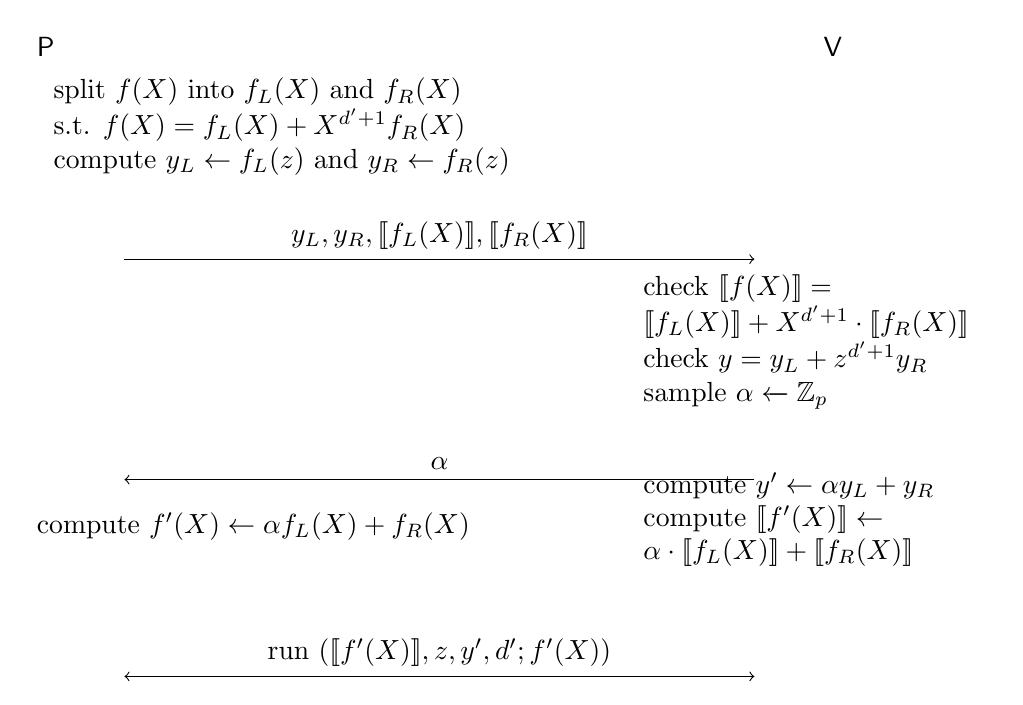
\begin{tikzpicture}
			\node[] (prover) at (-5, 0) {\prover};
			\node[] (verifier) at (5, 0) {\verifier};
			\node[anchor=north west] (prover computes) at (prover.south west) {\begin{tabular}{l}
				split $f(X)$ into $f_L(X)$ and $f_R(X)$ \\
				s.t. $f(X) = f_L(X) + X^{d'+1}f_R(X)$ \\
				compute $y_L \gets f_L(z)$ and $y_R \gets f_R(z)$
			\end{tabular}};
			\draw[->] (-4, -2.7) -- (4, -2.7) node[above, midway] {$y_L, y_R, [\![f_L(X)]\!], [\![f_R(X)]\!]$};
			\node[anchor=north west, xshift=-2.5cm, yshift=-2.5cm] (verifier checks) at (verifier.south west) {\begin{tabular}{l}
			check $[\![f(X)]\!] =$ \\
			 $[\![f_L(X)]\!] + X^{d'+1}\cdot [\![f_R(X)]\!]$ \\
			check $y = y_L + z^{d'+1}y_R$ \\
			sample $\alpha \xleftarrow{\dollar} \mathbb{Z}_p$
			\end{tabular}};
			\draw[->] (4, -5.5) -- (-4, -5.5) node[above, midway] {$\alpha$};
			\node[anchor=north west, yshift=-0.5cm] (verifier updates) at (verifier checks.south west) {\begin{tabular}{l}
				compute $y' \gets \alpha y_L + y_R$ \\
				compute $[\![f'(X)]\!] \gets$ \\
				$\alpha \cdot [\![f_L(X)]\!] + [\![f_R(X)]\!]$
			\end{tabular}};
			\node[anchor=north west, yshift=-4cm] (prover updates) at (prover computes.south west) {compute $f'(X) \gets \alpha f_L(X) + f_R(X)$};
			\draw[<->] (4, -8) -- (-4, -8) node[above, midway] {run $\eval([\![f'(X)]\!], z, y', d'; f'(X))$};
			\end{tikzpicture}
		\end{itemize}
		\end{flushleft}
\end{minipage}
\end{mdframed}
\end{figure}
\end{comment}

\begin{comment}
These operations give rise to the following informal pseudocode description of the \eval protocol.
\begin{mdframed}
Information-theoretic $\eval$ protocol, informal. \\
Common knowledge: $[\![f(X)]\!], y, z, d$ \\
Secret knowledge for \prover: $f(X)$ of degree $d$ \\
Statement: $y = f(z) \bmod p$ and $\deg(f(X)) = d$
	\begin{itemize}[nolistsep]
	    \item \textbf{if} $d > 0$ \textbf{then:}
		\item \pcind[1] \prover splits $f(X)$ into polynomials $f_L(X)$ and $f_R(X)$ of degree $d'=\frac{d+1}{2}-1$ such that $f(X) = f_L(X) + X^{d'+1}f_R(X)$
		\item \pcind[1] \prover sends $[\![f_L(q)]\!]$ and $[\![f_R(q)]\!]$ as well as $y_L \gets f_L(z) \bmod p$ and $y_R \gets f_R(z) \bmod p$ to \verifier
		\item \pcind[1] \verifier checks that $[\![f_L(q)]\!]+q^{d'+1} [\![f_R(q)]\!] = [\![f(q)]\!]$ and $y_L+z^{d'+1} y_R =y$
		\item \pcind[1] \verifier sends a random challenge $\alpha$ from $[-\frac{p-1}{2} ; \frac{p-1}{2}]$ to \prover
		\item \pcind[1] \prover and \verifier recurse on $[\![f'(q)]\!]=\alpha [\![f_L(q)]\!]+[\![f_R(q)]\!]$ for the statement $f'(z) = \alpha y_L + y_R \bmod p$ and $\deg(f'(X)) = d'$
		\item \textbf{if} $d=0$ \textbf{then:}
		\item \pcind[1] $\prover$ sends the constant $f$ to $\verifier$
		\item \pcind[1] $\verifier$ checks that $f$ is a small constant, that $[\![*]\!]$ evaluated in $f$ equals $[\![f]\!]$, and that $y = f \bmod p$
	\end{itemize}
\end{mdframed}
\end{comment}

\subsection{Integer Polynomial Encoding}

\label{sec:encoding}
We propose using integer commitments in a group of unknown order as a concrete instantiation of the homomorphic commitment scheme required for the abstract protocol presented in Section~\ref{sec:abstraction}. At the heart of our protocol is thus an encoding of integer polynomials with bounded coefficients as integers, which also has homomorphic properties. Any commitment scheme which is homomorphic over integer polynomials is automatically homomorphic over $\ZZ_p[X]$ polynomials as well (by reducing integer polynomials modulo $p$). Polynomials over $\ZZ_p[X]$ can be lifted to integer polynomials in a canonical way by choosing representatives in $[0,p)$. Therefore, from here on we will focus on building a homomorphic integer encoding of integer polynomials, and how to combine this with a homomorphic integer commitment scheme. 

\paragraph{Strawman encoding} In order to encode integer polynomials over an odd prime field $\mathbb{F}_p$, we first lift them to the ring of polynomials over the integers by choosing representatives in $[0,p)$. In the technical overview (Section~\ref{sec:overview}) we noted that a polynomial $f \in \ZZ[X]$ with positive coefficients bounded by $q$ can be encoded as the integer $f(q)$.   
The coefficients of $f$ can be recovered via the base $q$ decomposition of $f(q)$. 
This encoding is an injective mapping from polynomials in $\ZZ[X]$ of degree at most $d$ with positive coefficients less than $q$ to the set $[0, q^{d+1})$. The encoding is also \emph{partially} homomorphic. 
If $f$ is encoded as $f(q)$ and $g$ is encoded as $g(q)$ where coefficients of both $g, f$ are less than $q/2$, then the base-$q$ decomposition of $f(q) + g(q)$ gives back the polynomial $f + g$. 
By choosing a sufficiently large $q \gg p$ it is possible to perform several levels of homomorphic operations on encodings. 

\paragraph{What goes wrong?} Unfortunately, this simple encoding scheme does not quite work yet for the protocol outlined in Section~\ref{sec:overview}. The homomorphic consistency checks ensure that if $[\![f_L(X)]\!]$ is a homomorphic integer commitment to the encoding of $f_L \in \ZZ[X]$, $[\![f_R(X)]\!]$ is a homomorphic integer commitment to the encoding of $f_R \in \ZZ[X]$, and both $f_L, f_R$ are polynomials with $q/2$-bounded coefficients, then $[\![f(X)]\!]$ is an integer commitment to the encoding of $f_L + X^{d'}f_R$. (Moreover, if $f_L(z) = y_L \bmod p$ and $f_R(z) = y_R \bmod p$ then $f(z) = y_L + z^{d'} y_R \bmod p$). 

However, the validity of $[\![f_L(X)]\!]$ and $[\![f_R(X)]\!]$ are never checked directly. 
The verifier only sees the opening of the commitment at the bottom level of recursion. If the intermediate encodings use integer polynomials with coefficients larger than $q/2$ the homomorphism is not preserved. Furthermore, even if $[\![f(X)]\!]$ is a commitment to $f^*(q)$ with positive $q$-bounded coefficients, an adversarial prover could find an integer polynomial $g^*$ that does not have positive $q$-bounded coefficients such that $g^*(q) = f^*(q)$ and $g^* \not\equiv f^* \bmod p$ (\emph{i.e}, $g^*$ with coefficients greater than $q$ or negative coefficients). 
The prover could then commit to $g^*_L(q)$ and $g^*_R(q)$, and recurse on $\alpha g^*_L(q) + g^*_R(q)$ instead of $\alpha f^*_L(q) + f^*_R(q)$. This would be non-binding. (For example $f^*(X)= q-1$ and $g^*(X)=X-1$, or $f^*(X) = q +1$ and $g^*(X) = X + 1$). 

\paragraph{Inferring coefficient bounds} So what can the verifier infer from the opened commitment $[\![f']\!]$ at the bottom level of recursion? The opened commitment is an integer $f' = \alpha f_L + f_R$. From $f'$, the verifier can infer a bound on the absolute value of the coefficients of the integer polynomial $f(X) = f_L + X f_R$, given that $f_L$ and $f_R$ were already committed in the second to last round. The bound holds with overwhelming probability over the randomness of $\alpha \in [0,p)$. This is reasoned as follows: if $f'_0 \leftarrow \alpha_0 f_L + f_R$ and $f'_1 \leftarrow \alpha_1 f_L + f_R$ such that $\max(|f'_0|, |f'_1|) < q / (2p)$ for some distinct $\alpha_0 \neq \alpha_1$, then $|f_L| \leq |f'_1 - f'_0| < q / p$ and $|f_R| \leq |\alpha_0 f'_1 - \alpha_1 f'_0| < q/2$. If no such pair exists, \emph{i.e.} the bound only holds for a unique $\alpha$, then there is a negligibly small probability $1/p$ that $f'$ would have passed the bound check.


\paragraph{What about negative coefficients?} 
As shown above, the verifier can infer a bound on the absolute values of $f_L$ and $f_R$, but still cannot infer that $f_L$ and $f_R$ are both \emph{positive} integers. Moreover, if $f_R > 0$ and $f_L < 0$, then it is still possible that $f_L + q f_R > 0$, and thus that there is a distinct $g \neq f$ with $q$-bounded positive coefficients such that $g(q) = f(q)$. For example, say $f_R = q/2$ and $f_L = -1$ then $f_L + q f_R = q^2/2 - 1$, and $\alpha f_L + f_R  = q/2 - \alpha > 0$ for every $\alpha \in [0,p)$. Yet, also $q^2/2 - 1 = g(q)$ for $g(X) = (q/2 - 1)X + q-1$. 

\paragraph{Ensuring injectivity} How can we ensure the encoding scheme is injective over polynomials with either positive/negative coefficients bounded in absolute value? Fortunately, it is a fact that if $|f_L| < q/2$ and $|f_R| < q/2$ then at least one coefficient of $g$ must be larger than $q/2$. In other words, if the prover had committed instead to $f^*_L$ and $f^*_R$ such that $g(X) = f^*_L + Xf^*_R$ then the verifier could reject the opening of $\alpha \hat{f}^*_L + \hat{f}^*_R$ with overwhelming probability based on its size. 


More generally, for every integer $z$ in the range $B = (-\frac{q^{d+1}}{2}, \frac{q^{d+1}}{2})$ there is a unique degree (at most) $d$ integer polynomial $h(X)$ with coefficients whose absolute values are bounded by $q/2$ such that $h(q) = z$. \emph{We prove this elementary fact below and show how the coefficients of $h$ can be recovered efficiently from $z$ (Fact~\ref{EncodingBijective})}. If the prover is committed to $h(q)$ at level $i$ of the protocol, there is a unique pair of integers polynomial $h_L$ and $h_R$ with coefficients of absolute value bounded by $q/2$ such that $h_L(q) + q^{\frac{d+1}{2}} h_R(q) = h(q)$, and if the prover recurses on any other $h_L^*$ and $h_R^*$ with larger coefficients then the verifier's bound check at the bottom level of recursion will fail with overwhelming probability. 

\paragraph{Optimization with negative coefficients} As we have seen, an adversarial prover can commit to polynomials with positive or negative coefficients. As an optimization, we can actually allow the honest prover to encode polynomials using a mixture of negative and positive coefficients as well. A polynomial $f(X) \in \ZZ_p[X]$ is lifted to an integer polynomial by replacing each coefficient of $f$ with its unique integer representative from $(-p/2,p/2)$ of the same equivalence class modulo $p$. Also, $\alpha$ can be chosen from $(-p/2, p/2)$, leading to a tighter bound on coefficient growth. This leads us to the following encoding scheme. 

\paragraph{Final encoding scheme} Let $\ZZ(b):=\{x \in \ZZ: \vert x \vert  \leq b\}$ denote the set of integers with absolute value less than or equal to $b$.  Define $\ZZ(b)[X] := \{f \in \ZZ[X]: ||f||_\infty \leq b\}$, the set of integer polynomials with coefficients from $\ZZ(b)$. (For a polynomial $g \in \ZZ[X]$ the norm $||g||_\infty$ is the maximum over the absolute values of all individual coefficients of $g$.)
\begin{itemize} 

\item \textbf{Encoding.}
For any integer $q$, the function $\mathsf{Enc} : \mathbb{Z}(b)[X] \rightarrow \mathbb{Z}$ maps $h(X) \mapsto h(q)$. A polynomial $f(X) \in \ZZ_p[X]$ is first mapped to $\ZZ(p/2)[X]$ by replacing each coefficient of $f$ with its unique integer representative from $(-p/2,p/2)$ of the same equivalence class modulo $p$.  %This means the map can be used as encoding of polynomials in the domain $\ZZ(b)[X]$ with $b<q/2$.

\item \textbf{Decoding.}
Decoding works as follows. Define the partial sum $S_k := \sum_{i=0}^k f_i q^i$ with $S_{-1} := 0$. Assuming $|f_i| < q/2$ for all $i$, observe that for any partial sum $S_k$ we have $|S_k|<\frac{q^{k+1}}{2}$. Therefore, when $S_k < 0$ then $S_k \bmod q^{k+1} > q^{k+1}/2$ and when $S_k \geq 0$ then $S_k \bmod q^{k+1} < q^{k+1}/2$. 
This leads to a decoding strategy for recovering $S_k$ from $y \in \mathbb{Z}$. The decode algorithm sets $S_k$ to $y \bmod q^{k+1}$ if this value is less than $q^{k+1}/2$ and to $q^{k+1}- (y \bmod q^{k+1})$ otherwise.
Two consecutive partial sums yield a coefficient of $f(X)$: $f_k = \frac{S_{k} - S_{k-1}}{q^{k}} \in \ZZ(b)$. These operations give rise to the following algorithm.\\
\end{itemize}

 \begin{minipage}{\textwidth}
\begin{mdframed}
\begin{flushleft}
	$\pro{Dec}(y \in \mathbb{Z}):$
	\begin{enumerate}[nolistsep]
	    \item \textbf{for each} $k$ \textbf{in} $[0, \, \lfloor \log_q(|y|)\rfloor]$ \textbf{do:}\\
		\item \pcind[1] $S_{k-1} \gets (y \bmod q^{k})$
		\item \pcind[1] \pcif{$S_{k-1} > q^{k}/2$} \textbf{then} $S_{k-1} \gets q^{k}-S_{k-1}$ \textbf{end if}
		\item \pcind[1] $S_k \gets (y \bmod q^{k+1})$
		\item \pcind[1] \pcif{$S_{k} > q^{k+1}/2$} \textbf{then} $S_{k} \gets q^{k+1}-S_{k}$ \textbf{end if}
		\item \pcind[1] $f_k \gets (S_{k} - S_{k-1}) / q^k$
		\item \pcreturn $f(X) = \sum_{k=0}^{\lfloor \log_q(|y|)\rfloor} f_k X^k$
	\end{enumerate} 
\end{flushleft}
\end{mdframed}
\end{minipage}

\begin{fact} \label{EncodingBijective}
Let $q$ be an odd integer. For any $z$ in the range $B = (-\frac{q^{d+1}}{2}, \frac{q^{d+1}}{2})$ there is a unique degree (at most) $d$ integer polynomial $h(X)$ in $\ZZ(\frac{q-1}{2})[X]$ such that $h(q) = z$. 
\end{fact}
\begin{proof}
Given any degree (at most) $d$ integer polynomial $f \in \ZZ(\frac{q-1}{2})$, by construction we see that $\pro{Dec}(\pro{Enc}(f)) = f$. Therefore, $\pro{Enc}$ is an injective map from degree (at most) $d$ polynomials in $\ZZ(\frac{q-1}{2})[X]$ to $B$. Furthermore, the cardinality of both the domain and range of this map is $q^{d+1}$. This shows that the map is surjective. In conclusion, the map is bijective. 
\end{proof}

\paragraph{Encoding of dyadic rational polynomials.}
\benedikt{This really needs to go}
There exists an algorithm to compute square roots of any element of a class group of an imaginary quadratic order, originally described by Gauß (see Bosma and Stevenhagen for a modern description~\cite{jtn/BosSte96}). As a result, in such class groups an adversary can also commit to \defn{dyadic rationals} $\mathbb{D}:=\{\frac{x}{2^k} : \ x \in \ZZ \wedge k \in \NN\}\subset \QQ$, in addition to integers. When using class groups we therefore need to modify the encoding scheme . 

The encoding map is identical, except lifted to the dyadic rationals: $\mathsf{Enc} : \mathbb{D}[X] \rightarrow \mathbb{D}, \, g(X) \mapsto g(q)$. The main difference with respect to the integer encoding scheme will be that decoding works for dyadic rationals where \emph{both the numerator and the denominator are bounded}. Let $N \in \NN$ be a bound on the absolute value of the numerator and $2^D\in \NN$ be a bound on the value of the denominator, and let $\mathbb{D}(N, D) :=\{\frac{x}{2^a} \in \mathbb{D} : \ |x|\leq N \wedge 2^a \leq D\}$ denote the set of such bounded dyadic rationals. The encoding scheme is uniquely decodable if $N \cdot 2^a < q/2$.
 
Note that denominator of $g(q)$ is bounded by $2^{\lfloor\log_2(D)\rfloor}$, $D$ rounded down to the next power of $2$. To decode such a dyadic rational, compute the integer $y \gets g(q) \cdot 2^{\lfloor\log_2(D)\rfloor}\in \ZZ$  and use the decoding algorithm described above to decode a polynomial $f(X)$ in $\ZZ(q/2)[X]$. From $f(X)$ one derives the polynomial  $g(X) \gets \frac{f(X)}{2^{\lfloor\log_2(D)\rfloor}} \in \mathbb{D}(\lceil q/(2D)\rceil, 2^{\lfloor\log_2(D)\rfloor})[X]$ through division. If the integer polynomial encoding is uniquely decodable, then so is the scheme for dyadic rational polynomials. If $q$ is a power of $2$, then an adversary can encode Laurent polynomials, \emph{i.e.}, polynomials where some terms have negative powers. In order to disallow negative powers, $q$ must be odd.

\subsection{Concrete Polynomial Commitment Scheme}
\label{subsec:concretepoly}
We now instantiate the abstract homomorphic commitment function $[\![ * ]\!]$. To this end we sample a group of unknown order $\mathbb{G}$, and sample a random element $\gr{g}$ from this group. 
Lift the field polynomial $f(X)\in \ZZ_p[X]$ to an integer polynomial with bounded coefficients, \emph{i.e.}, $\hat{f}(X)\in \ZZ(\frac{p-1}{2})[X]$ such that $\hat{f}(X)\bmod p=f(x)$.
We encode $\hat{f}(X)$ as an integer by evaluating it at a ``large enough'' integer $q$. Finally we use exponentiation in $\GG$ to commit to the integer. Therefore, $[\![f(X)]\!]$, corresponds to $\gr{g}^{\hat{f}(q)}$. This commitment function inherits the homomorphic properties of the integer encoding for a limited number of additions and multiplications-by-constant. The monomial homomorphism for $X^d$ is achieved by raising the group element to the power $q^{d}$. To maintain consistency between the prover's witness polynomials and the verifier's commitments, the prover operates on polynomials with integer coefficients  $\hat{f}(X), \hat{g}(X)$, \emph{etc.}, without ever reducing them modulo $p$.

The $\setup, \pro{Commit}$ and $\open$ functionalities are presented formally below. Note that the scheme is parameterized by $p$ and $q$.
%; these values are determined by the context and independently of $\setup$.

%We now present our main technical contribution: a polynomial commitment scheme with an efficient evaluation protocol based on a group of unknown order $\GG$. For polynomials of degree $d=\poly$ the evaluation protocol uses $1+\lceil\log_2(d+1)\rceil$ rounds and $O(\log(d))$ communication and verifier work.

%Exponentiation in groups of unknown order is a succinct and homomorphic cryptographic commitments to an integer.
%Using the integer encoding of polynomials, or their encoding as dyadic rationals, above we can simply commit to a polynomial $f(X)$ with bounded coefficients by computing $\gr{g}^{f(q)} \in \GG$. Every polynomial in $\ZZ_p[X]$ naturally maps to an integer polynomial with coefficients in $B_{\frac{p-1}{2}}$. The commitment scheme, therefore, supports committing to polynomials in $\ZZ_p[X]$ for $p \leq q$. Interestingly, neither $p$ nor the degree $d$ need to be specified in the setup. 

%As long as $q$ and ``big enough'' they can be freely chosen.\alan{Todo: make this observation elsewhere.} %In class groups there is an efficient algorithm to compute square roots, and as a result, a prover can also commit to dyadic rationals. Since every dyadic rational corresponds to a unique element in $\ZZ_p$ we can simply extend the encoding to work for polynomials with bounded dyadic rational coefficients. The only difference is that we require $q$ to be odd such that the prover cannot commit to polynomials with negative powers. We will discuss the relationship between $p$, $d$ and $q$ in more detail later but first we describe the setup, commitment and opening algorithms:

\begin{itemize}
\item $\pro{Setup}(1^\secpar):$ Sample $ \GG \sample \ggen(\secpar)$
			and $ \gr{g} \sample \GG$. Return $\params = (\secpar,\GG,\gr{g}, q)$.
\item $\pro{Commit}(\params;f(X) \in \ZZ_p[X]):$ Compute $\gr{C} \gets \gr{g}^{\hat{f}(q)}$ and return $(\gr{C};\hat{f}(X))$.
\item $\pro{Open}(\params,\gr{C}, f(X), \hat{f}(X)):$ Check that $\hat{f}(X)\in \ZZ(q/2)[X]$ and $\gr{g}^{\hat{f}(q)} = \gr{C}$ and $f(X) = \hat{f}(X) \bmod p$. 
\end{itemize}

\begin{comment}
\begin{small}
\begin{mdframed}[userdefinedwidth=\textwidth]
\begin{minipage}{\textwidth}
	\begin{flushleft}
	$\pro{Setup}(1^\secpar):$
		\begin{enumerate}[nolistsep]
			\item $ \GG \sample \ggen(\secpar)$
			\item $ \gr{g} \sample \GG$
			%\item $q \gets 2^k$ such that $q > (d+1) \cdot 2\cdot p^{\log_2(d+1)+1} $
			%\item Pick a prime $p\in \NN$ such that $\lceil\log_2(p)\rceil=\lambda$.
			%\item Pick a sufficiently large and odd $q\in \NN$ (See discussion above)
			%\item $\pcreturn \params = (\secpar,\GG,\gr{g},p,q)$
			\item $\pcreturn \params = (\secpar,\GG,\gr{g})$
		\end{enumerate}
	$\pro{Commit}(\params;f(X) \in \ZZ(p)[X]):$ \pccomment{$f(X)\equiv \tilde{f}(X) \mod p$ for  $\tilde{f}(X)\in \ZZ_p[X]$}
		\begin{enumerate}[nolistsep]
			\item $\gr{C} \gets \gr{g}^{f(q)}$
			\item $\pcreturn (\gr{C};f(X))$
		\end{enumerate}
	$\pro{Open}(\params,\gr{C}, f(X)):$ \pccomment{$f(X) \in \ZZ(b)[X]\subset\mathbb{Z}[X]$ for $b<q/2$}
		\begin{enumerate}[nolistsep]
		    \item \prover sends $f(X)$ to \verifier.
		   % 				\item \verifier checks that $\tilde{f}(X) = f(X) \mod p$
		    \item \verifier checks that $f(X)\in \ZZ(b)[X]$ and $b<q/2$
			\item \verifier checks that $\gr{g}^{f(q)} = \gr{C}$ \pccomment{Can be outsourced using $\textsf{PoE}(\gr{g},\gr{C},f(q))$}
			\item \pcif all checks pass \textbf{then} \pcreturn $1$ \textbf{else} \pcreturn $0$
		\end{enumerate}
		\end{flushleft}
\end{minipage}
\end{mdframed}
\end{small}
\end{comment}
%Opening the commitment can be simply done by rerunning the commitment algorithm. Additionally a proof of exponentiation (PoE) can be used to increase verifier efficiency.
%The commitment inherits the homomorphic properties of the integer encoding. Assume that we are committing to representations of polynomials in $\ZZ_p[X]$, \emph{i.e.}, polynomials with coefficients bounded by $p$. Then the commitment scheme supports up to $\frac{q}{p}$ homomorphic additions. Equivalently, when raising a commitment to a weight $\alpha$, the size of the coefficients grows by at most a factor of $|\alpha|$. We use this property to build an efficient $\eval$ protocol. 

%The core idea of the $\eval$ protocol is to reduce the statement from one about a polynomial $f(X)$ of degree $d$ to one about a polynomial of degree $d'=\frac{d+1}{2}-1$. For simplicity assume that $d+1$ is a power of $2$.
%The prover splits $f(X)$ into $f_L(X)$ and $f_R(X)$ such that $f(X) = f_L(X)+X^{d'+1} f_R(X)$ and such that both polynomials have degree at most $d'$. Then he proves that $f'(X)=\alpha \cdot f_L(X) + f_R(X)$ has degree $d'$ for a random challenge $\alpha\in [-\frac{p-1}{2},\frac{p-1}{2}]$. 

%If the prover wants to show, in addition to the previous, that $f(z)=y\bmod p$, then he can simply provide $y_L=f_L(z)\bmod p$ and $y_R=f_R(z)\bmod p$ and show that $y_L + z^{d'+1} \cdot y_R \bmod p=y$. Note that the verifier can compute $y' = f'(z) = \alpha \cdot y_L + y_R \bmod p$ from $y_L$ and $y_R$.

%The proof recursively repeats this reduction by using $f'(X),z,y'$ and $d'$ as the input. In the final step, the prover simply sends the constant polynomial $f$ and the verifier can check that $f \equiv y \bmod p$. Note that $|f|< (\frac{p}{2})^{\log_2(d+1)+1}$ so an integer encoding of $f_0$ requires at most $\lceil \log_2(d+1) \cdot \log_2(p)\rceil$ bits. 
\paragraph{Evaluation protocol}
Using the cryptographic compilation of the information theoretic protocol we get an $\eval$ protocol with logarithmic communication. In every round, however, the verifier needs to check consistency between $[\![f_L(X)]\!],[\![f_R(X)]\!]$ and $[\![f(X)]\!]$. This is done by checking that $\gr{C}_L \cdot \gr{C}_R^{q^{d'+1}}=\gr{C}$. This naive check is highly inefficient as the exponent $q^{d'+1}$ has $O(d)$ bits.
%For the concrete evaluation protocol, one starts with the situation in which the verifier possesses a commitment to $f(X)$ in the form of $\gr{C} = \gr{g}^{f(q)}$. The prover commits to $f_L(X)$ and $f_R(X)$ by sending $\gr{C}_L$ and $\gr{C}_R$. The verifier checks that $\gr{C} = \gr{C}_L \cdot \gr{C}_R^{q^{d'+1}}$ and proceeds in the next step with the commitment $\gr{C}' = \gr{C}_L^\alpha \cdot \gr{C}_R$ to $f'(X)$. This instantiation produces an $\eval$ protocol with logarithmic communication. However, naïvely checking that $f(X) = f_L(X) + X^{d'+1} f_R(X)$ based on the commitments $\gr{C}, \gr{C}_L$ and $\gr{C}_R$ is inefficient because the bit-size of the exponent $q^{d'+1}$ is huge.
To resolve this inefficiency, we utilize a proof of exponentiation (\textsf{PoE})~\cite{ITCS:Pietrzak18,EC:Wesolowski19} to outsource the computation to the prover.
The \textsf{PoE} protocol is an argument that a large exponentiation in a group of unknown order was performed correctly. Wesolowski's \textsf{PoE}~\cite{EC:Wesolowski19} is public coin, has constant communication and verification time, and is thus particularly well-suited here.

We now specify subtleties that were previously glossed over. 
First, we handle the case where $d+1$ is not a power of 2.  Whenever $d+1$ is odd in the recursion, the polynomial is shifted by one degree --- specifically, $f'(X) = X f(X)$ and the protocol proceeds to prove that $f'(X)$ has degree bounded by $d' = d+1$ and evaluates to $y' = zy$ at $z$. The verifier obtains the matching commitment $\gr{C}'\gets\gr{C}^q$.

Second, the coefficients of $f(X)$ grow by a factor of $\frac{p+1}{2}$ in every recursion step, but eventually the transmitted constant $f$ has to be tested against some bound because if it is \emph{too large} it should be rejected. However, the function interface provides no option to specify the allowable size of coefficients. We therefore define and use a subroutine $\pro{EvalBounded}$, which takes an additional argument $b$ and which proves, in addition to what $\pro{Eval}$ proves, that all coefficients $f_i$ of $f(X)$ satisfy $|f_i| \leq b$. Importantly, $b$ grows by a factor for $\frac{p+1}{2}$ in every recursion step. This subroutine is also useful if commitments were homomorphically combined prior to the execution of $\pro{EvalBounded}$. The growth of these coefficients determines a lower bound on $q$: $q$ should be \emph{significantly} larger than $b$. Exactly which factor constitutes ``significantly'' is determined by the knowledge-soundness proof.

In the final round we check that the constant $f$ satisfies $|f|\leq b$ and the protocol's correctness is guaranteed if $b = \frac{p-1}{2}(\frac{p+1}{2})^{\lceil\log_2(d+1)\rceil}$. However, $q$ needs to be even larger than this value in order for extraction to work (and hence, for the proof of witness-extended emulation to go through). In RSA groups, where computing square roots is hard, we need $q>p^{2\log(d+1)+1}$; whereas in class groups where computing square roots is easy, we need $p^{3\log(d+1)+1}$. When this condition is satisfied, we can prove that the original committed polynomial has coefficients smaller than $\frac{q}{2}$. To avoid presenting two algorithms whose only difference is the one constant, we capture this constant explicitly in the variable $\boldsymbol{\varsigma}_{p,d}$ and set its value depending on the context:
\benedikt{Update}
\[
    \boldsymbol{\varsigma}_{p, d} = \left\{
        \begin{array}{ll}
            p^{\,\log_2(d+1)} & \quad \textnormal{(in RSA groups)} \\
            p^{\,2\log_2(d+1)} & \quad \textnormal{(in class groups)}
        \end{array}
    \right. \enspace .
\]

 We now present the full, formal $\eval$ protocol below.
%\begin{small}
\begin{mdframed}
\begin{minipage}{\textwidth}
			$\pro{Eval}(\crs, \gr{C}\in \GG, z\in \ZZ_p, y\in \ZZ_p, d \in \NN; \tilde{f}(X)\in \ZZ_p[X]) :$ \pccomment{$\tilde{f}(X) = \sum_{i=0}^d \tilde{f}_i X^i$}
			\begin{enumerate}[nolistsep]
			\item \prover computes $f_i \in [-\frac{p-1}{2},\frac{p-1}{2}]$ such that $f_i\equiv \tilde{f}_i\bmod p$ for all $i\in[0,d]$.
			\item \prover computes $f(X)\gets \sum_{i=0}^d f_i \cdot X^{i}\in \ZZ(\frac{p-1}{2})[X]\subset \ZZ[X]$
			\item \prover and \verifier run $\pro{EvalBounded}(\params,\gr{C},z,y,d,\frac{p-1}{2};f(X))$
		    \end{enumerate}
		    		\vspace{1em}
		$\pro{EvalBounded}(\crs,\gr{C}\in \GG,z\in \ZZ_p,y\in \ZZ_p,d\in \NN,b\in \ZZ;f(X)\in \ZZ(b)[X])$		
	    \begin{enumerate}[nolistsep]
        \item \pcif $d=0$:
        \item \label{line:basestart}\pcind[1] \prover sends $f(X)\in \ZZ$ to the verifier. \pccomment{$f=f(X)$ is a constant}

        \item \pcind[1] \verifier checks that $b\cdot \boldsymbol{\varsigma}_{p,d} < q$\pccomment{$\boldsymbol{\varsigma}_{p,d}=O(p^{2\log(d)})$ (see Theorem~\ref{thm:polycommitsecurity} and \ref{thm:dyadicpolysecurity})}
        %q/(2^{\lceil \log_2(d+1) \rceil+1} p^{2 \lceil \log_2(d+1) \rceil+1})$
        \item \pcind[1] \verifier checks that $|f|\leq b$
          \item \pcind[1] \verifier checks that $f\equiv y \bmod p$
                \item \label{line:baseend}\pcind[1] \verifier checks that $\gr{g}^{f}=\gr{C}$
\item \pcind[1] \verifier outputs $1$ \pcif all checks pass, $0$ otherwise.
          \item \pcif{$d+1$ is odd}
         \item \pcind[1]  $d'\gets d+1, \gr{C}'\gets \gr{C}^q$, $y'\gets y\cdot z \bmod p$ and $f'(X)\gets X \cdot f(X)$.
         \item \pcind[1] \prover and \verifier run $\pro{EvalBounded}(\crs,\gr{C}',z,y',d',b;f'(X))$

        \item \pcelse: \pccomment{$d \geq 1$ and $d+1$ is even}
       
        \item \pcind[1] \prover and \verifier compute $d' \gets \frac{d+1}{2} - 1$
        \item \pcind[1] \prover computes $f_L(X) \gets \sum\limits_{i=0}^{d'} f_i \cdot X^i$ and $f_R(X)\gets\sum\limits_{i=0}^{d'} f_{d'+1+i}\cdot X^{i}$
        \item \pcind[1] \prover computes $y_L\gets f_L(z) \bmod p$ and $y_R\gets f_R(z)\bmod p$
        \item \pcind[1] \prover computes $\gr{C}_L \gets \gr{g}^{f_L(q)}$ and $\gr{C}_R \gets \gr{g}^{f_R(q)}$
        \item \pcind[1] \prover sends $y_L,y_R, \gr{C}_L, \gr{C}_R$ to \verifier. \pccomment{See Section \ref{subsec:optimization} for an optimization}
        \item \pcind[1] \verifier checks that $y=y_L+z^{d'+1}\cdot y_R \bmod p$, outputs $0$ if check fails.
        \item \pcind[1] \label{line:PoE} \prover and \verifier run $\pro{PoE}(\gr{C}_R, \gr{C}/\gr{C}_L, q^{d'+1})$\pccomment{Showing that $\gr{C}_L\gr{C}_R^{(q^{d'+1})}=\gr{C}$}
        \item \pcind[1] \verifier samples $\alpha \sample [-\frac{p-1}{2},\frac{p-1}{2}]$ and sends it to \prover
        \item \pcind[1] \prover and \verifier compute $y'\gets\alpha  y_L +y_R \bmod p$, $\gr{C}' \gets \gr{C}_L^\alpha  \gr{C}_R$, $b'\gets b \frac{p+1}{2}$. 
        \item \pcind[1] \prover computes $f'(X) \gets \alpha \cdot f_L(X) + f_R(X) \in \ZZ[X]$ \pccomment{$\deg(f'(X))=d'$}
        \item \pcind[1] \prover and \verifier run $\pro{EvalBounded}(\params, \gr{C}', z, y', d',b' ; f'(X))$
               \end{enumerate}
      \end{minipage}
\end{mdframed}
%\end{small}


\begin{comment}
\end{comment}

\subsection{Security Analysis} 
 \newcommand{\bindinglemma}{
 The polynomial commitment scheme is binding for polynomials in $\ZZ(b)[X]$ for $b<q/2$ if either the Adaptive Root Assumption or the Strong RSA Assumption hold.
	}
\begin{lemma}
\label{lem:binding}
	\bindinglemma
	\end{lemma}

\newcommand{\correctnesslemma}{
The polynomial commitment scheme is correct for polynomials in $\ZZ_p[X]$ of degree at most $d$ if $q> p^{\lceil \log_2(d+1)\rceil+1}$.
}
 
 \begin{lemma}
 	\label{lem:correctness}
\correctnesslemma
 \end{lemma}


The proofs of the previous lemmas are in Appendix~\ref{appendix:binding} and \ref{appendix:correctness}.
Next is the main security theorem, which states that the evaluation protocol has witness-extended emulation. We start with a high-level intuitive overview where we also identify potential obstacles.

\paragraph{Proof idea.} %Consider the information theoretic version of the $\eval$ protocol, where the prover sends the integer polynomials $f_L(X)$ and $f_R(X)$ in each round but the verifier does not read them.
The goal is to construct an extractor by recursively computing $f(X)$ from $f'(X)$. In the final round the verifier receives $f$ such that $|f| \leq b$, and therefore the extractor possesses this constant polynomial as well. Working backwards from here, the extractor uses rewinding in every step to find $f_L(X)$ and $f_R(X)$ and thereby finds $f(X) = f_L(X) + X^{d'+1}f_R(X)$.
Specifically, in each round the extractor has $f'(X)=\alpha f_L(X)+ f_R(X)$. Suppose the extractor also possesses $f''(X)=\alpha' f_L(X)+ f_R(X)$. From $f'(X)$, $f''(X)$, $\alpha$ and $\alpha'$ it is easy to compute $f_L(X)$ and $f_R(X)$. The extractor then computes $f(X)=f_L(X)+X^{d'+1} f_R(X)$.
A careful analysis shows that if the coefficients of $f'(X)$ are bounded by $b$ then $f_L(X)$ and $f_R(X)$ must have coefficients bounded by $b \cdot p$ in absolute value. Using a similar analysis we can show that $f(z)\bmod p=y$ for the extracted polynomial $f(X)$.

This argument shows that there is an extractor algorithm $\mathcal{X}$ capable of extracting the witness $f(X)$ from a binary tree of accepting transcripts. Moreover, a tree-finding algorithm $\mathcal{T}$ can output such a tree by repeatedly rewinding the prover, running it with fresh verifier randomness each time, and recording the resulting transcripts. As a result, the Generalized Forking Lemma (Lemma~\ref{lemma:GFL}) applies and establishes that the protocol has witness-extended emulation.

The full proof takes into account the cryptographic compilation of the protocol using the integer encoding and the commitment scheme based on groups of unknown order. Additionally the full proof will need to support dyadic rationals because taking square roots is easy in class groups.





%We are now in a position to prove the main security statement.

\newcommand{\maintheorem}{
The polynomial commitment scheme for polynomials in $\ZZ_p[X]$ of degree at most $d=\poly$, instantiated using $q>p^{2\lceil \log_2(d+1)\rceil+1}$ and $\ggen$, has witness extended emulation (Definition \ref{def:wee}) if the Adaptive Root Assumption and the Strong RSA Assumption hold for $\ggen$.
}
\begin{theorem}~\label{thm:polycommitsecurity} 
	\maintheorem
\end{theorem}

%\textit{Remark:}
%The bound on $q$ for correctness (Lemma \ref{lem:correctness}) is $O((\frac{p}{2})^{\log(d)})$ while the bound for soundness is $O((\frac{p}{2})^{2 \log(d)})$. It is not clear whether this gap can be closed. While the soundness analysis is tight for the worst case assumption on challenges it is possible that a probabilistic analysis could give a tighter result.

\newcommand{\dyadicmaintheorem}{
Let $\ggen$ generate groups $\GG$ of unknown order such that the order of $\GG$ is odd, and such there exists a PPT algorithm for taking square roots in $\GG$. The polynomial commitment scheme for polynomials in $\ZZ_p[X]$ of degree at most $d=\poly$, instantiated using $q>p^{3\lceil \log_2(d+1)\rceil +1}$ and $\ggen$, has witness extended emulation (Definition \ref{def:wee}) if the Adaptive Root Assumption and the  $2$-Strong RSA Assumption hold for $\ggen$.
}
\begin{theorem}
\label{thm:dyadicpolysecurity}	
\dyadicmaintheorem
\end{theorem}
The proof of Theorem~\ref{thm:dyadicpolysecurity} is nearly identical to the proof of Theorem~\ref{thm:polycommitsecurity} but the extracted polynomials are polynomials over the dyadic rationals and not over the integers. This requires the bound on $q$ to be larger by a factor of $p^{\log(d+1)}$. Both proofs are presented in the \appendixphrase~(\ref{appendix:maintheoremproof} and \ref{apx:dyadic}).


\subsection{Optimizations}
\label{subsec:optimization}
We present several ideas for optimizing the performance of the $\pro{Eval}$ protocol.

\paragraph{Precomputation.} The prover has to compute powers of $\gr{g}$ as large as $q^d$. While this can be done in linear time, this expense can be shifted to a preprocessing phase in which all elements $\gr{g}^{q^i}, i \in \{1, \ldots, d_{\it max}\}$ are computed. Since for coefficient $|f_i|\leq -\frac{p-1}{2}$ this allows the computation of $\gr{g}^{f(q)}$ in $O(\lambda d)$ group operations as opposed to $O(\lambda d \log(d))$.
In addition to reducing the prover's workload, this optimization enables parallelizing it. The computation of the $\textsf{PoE}$ proofs can simiarly be parallelized. The prover can express each $Q$ as a power of $\gr{g}$ which enables pre-computation of powers of $\gr{g}$ and parallelism as described by Boneh~\emph{et al.}~\cite{C:BonBunFis19}.
%The elements $\gr{g}^{q^i}$ can themselves be accompanied by non-interactive $\mathsf{PoE}$s to establish their correct computation.

The pre-computation also enables the use of multi-scalar multiplication techniques~\cite{pippenger1980evaluation}. Boneh~\emph{et al.}~\cite{C:BonBunFis19} and Wesolowski~\cite{EC:Wesolowski19} showed how to use these techniques to reduce the complexity of the $\textsf{PoE}$ prover. The largest $\textsf{PoE}$ exponent $q^{\frac{d+1}{2}}$ has $O(\lambda d \log(d))$ bits. Multi-scalar multiplication can therefore reduce the prover work to $O(\lambda d)$ instead of $O(\lambda d \log(d))$.

%\paragraph{Early termination.} The protocol specifies the recursion ends when $d=0$, but the communication cost might be reduced if it terminates earlier. This reduction holds when the size of the fewer group elements $\gr{C}_L$ and $\gr{C}_R$ outweigh the size of the larger polynomial $f(X)$ instead of the constant $f$.

%\paragraph{Fiat-Shamir.} All the challenges of the verifier are public coin and as a result the protocol can be made non-interactive in the random oracle model with the Fiat-Shamir heuristic~\cite{C:FiaSha86}. This technique replaces each message of the verifier with the hash of all previous protocol messages, lifted to the appropriate domain. For the \textsf{PoE}s, it is beneficial to reuse the same $\ell$ across all \textsf{PoE}s and to compute this prime as the hash of the entire transcript after (dropping the $\ell$s and) replacing every instance of $\gr{Q}$ by its matching $\gr{C}_R^{q^{d'+1}}$ counterpart. This optimization requires that $\ell$ be transmitted as part of the proof so that the verifier can infer the $\gr{C}_R^{q^{d'+1}}$ and $\gr{C}_L$, and only after this inference can the verifier check that $\ell$ was computed correctly. The concrete benefit of this optimization is the reduced work for the verifier: previously he had to perform $\lceil\log(d+1)\rceil$ exponentiations of $q \bmod \ell$ to the power $d'+1$, whereas now he can do this task once and record the intermediate results.

\paragraph{Two group elements per round.} In each round the verifier has a value $\gr{C}$ and receives $\gr{C}_L$ and $\gr{C}_R$ such that $\gr{C}_L+q^{d'+1}\cdot \gr{C}_R=\gr{C}$. This is redundant. It suffices that the verifier sends $\gr{C}_R$. The verifier could now compute $\gr{C}_L\gets \gr{C} -q^{d'+1} \gr{C}_R$, but this is expensive as it involves an scalar multiplication by $q^d$. Instead, the verifier infers $q^{d'+1}\cdot \gr{C}_R$ from the \textsf{PoE}: the prover's message is $\gr{Q}$ and the verifier can directly compute $q^{d'+1}\cdot \gr{C}_R\gets \ell \cdot \gr{Q}+r\cdot \gr{C}_R$ for a challenge $\ell$ and $r\gets q^{d'+1} \bmod \ell$. From this the verifier infers $\gr{C}_L \gets \gr{C}-q^{d'+1} \cdot \gr{C}_R$. The security of $\textsf{PoE}$ does not require that $q^{d'+1}\cdot \gr{C}_R$ be sent before the challenge $\ell$ as it is uniquely defined by $\gr{C}_R$ and $q^{d'+1}$.
The same optimization can be applied to the non-interactive variant of the protocol. 

Similarly the verifier can infer $y_L$ as $y_L\gets y-z^{d'+1} y_R$. This reduces the communication to two group elements per round and 1 field element. Additionally the prover sends $f$ which has roughly the size of $\log(d+1)$ field elements, which increases the total communication to roughly $2\log(d)$ elements in $\GG$ and $2\log(d)$ elements in $\ZZ_p$. 

%When the $\mathsf{PoE}$s are made non-interactive, the prover can get away with producing only two group elements instead of three. With a naïve application of the Fiat-Shamir heuristic, the $\mathsf{PoE}$ proof consists of $(\gr{C}_R, \gr{C}_R^\star, \gr{Q})$ where $\gr{Q}$ is determined by $\ell$, which in turn is determined by hashing all previous protocol messages: $\ell \gets \mathsf{H}(\cdot \Vert \gr{C}_R \Vert \gr{C}_R^\star)$. The optimization sends $(\gr{C}_R, \gr{Q}, \ell)$ instead. The verifier can infer $\gr{C}_R^\star = \gr{C}_R^{(q^{d'+1} \bmod \ell)}$ and then test $\mathsf{H}(\cdots \Vert \gr{C}_R \Vert \gr{C}_R^\star) \stackrel{?}{=} \ell$. This optimization is particularly compatible with the previous batching of $\mathsf{PoE}$s optimization, because while there is a unique $\gr{Q}$ for each round, there need only be one $\ell$ for the entire $\eval$ protocol.

\paragraph{Evaluation at multiple points}
The protocol and the security proof extend naturally to the evaluation in a vector of points $\boldsymbol{z}$ resulting in a vector of values $\boldsymbol{y}$, where both are members of $\mathbb{Z}_p^k$. The prover still sends $\gr{C}_L\in \GG$ and $\gr{C}_R\in \GG$ in each round and additionally $\boldsymbol{y}_L,\boldsymbol{y}_R \in \ZZ^k_p$. In the final round the prover only sends a single integer $f$ such that $\gr{g}^{f}=\gr{C}$ and $f \bmod p=y$.

This is significantly more efficient than independent executions of the protocol as the encoding of group elements is usually much larger than the encoding of elements in $\ZZ_p$. Using the optimization above, the marginal cost with respect to $k$ of the protocol is a single element in $\ZZ_p$. If $\lambda=\lceil\log_2(p)\rceil$ is $120$, then this means evaluating the polynomial at an additional point increases the proof size by only $15\log(d+1)$ bytes.

\paragraph{Joining $\mathsf{Eval}$s.} 
In many applications such as compiling polynomial IOPs to SNARKs (see Section~\ref{sec:polyiop}) multiple polynomial commitments need to be evaluated at the same point $z$. 
This can be done efficiently by taking a random linear combination of the polynomials and evaluating that combination at $z$. The prover simply sends the evaluations of the individual polynomials and then a single evaluation proof for the combined polynomials. The communication cost for evaluating $m$ polynomials at $1$ point is still linear in $m$ but only because the evaluation of each polynomial at the point is being sent. The size of the eval proof, however, is independent of $m$. 
Taking a random linear combination does increase the bound on $q$ slightly, as shown in Theorem~\ref{thm:joined} which is presented below.

\[
\mathcal{R_\textsf{JE}}(\params) = \left\lbrace
\langle (\gr{C}_1,\gr{C}_2, z, y_1,y_2,d), (f_1(X), f_2(X)) \rangle
: \\
\begin{array}{l} 
\gr{C}_1, \gr{C}_2 \in \GG \\
z, y_1, y_2 \in \mathbb{Z}_p \\
f_1(X), f_2(X) \in \ZZ(b) \\
(\gr{C}_1,z,y_1,d) \in \mathcal{R_\textsf{Eval}}(\params) \\
(\gr{C}_2,z,y_2,d) \in \mathcal{R_\textsf{Eval}}(\params)
\end{array}
\right\rbrace
\]





\begin{mdframed}
	$\pro{JoinedEval}(\crs, \gr{C}_1, \gr{C}_2, z, y_1, y_2, d; f_1(X),f_2(X)) :$ \pccomment{$f_1(X), f_2(X) \in \ZZ(\frac{p-1}{2})[X]$} \\
%	Statement: $f_1(z)=y_1\bmod p \wedge f_2(z)=y_2\bmod p \wedge \gr{g}^{f_1(q)}=\gr{C}_1$ and $\gr{g}^{f_2(q)}=\gr{C}_2$
Statement: $(\crs,\gr{C}_1,\gr{C}_2,z,y_1,y_2,b,d)\in \mathcal{R}_{\pro{JE}}$
			\begin{enumerate}[nolistsep]
			\item $b=||f_1,f_2||_\infty$
        \item \verifier samples $\alpha \sample [0,2^\lambda)$ and sends it to \prover
			\item \prover and \verifier compute $\gr{C}'\gets \alpha \cdot \gr{C}_1+\gr{C}_2$ and $y'\gets \alpha \cdot y_1 +y_2 \bmod p$
			\item \prover computes $f'(X)\gets \alpha f_1(X) +f_2(X)$
			\item \prover and \verifier run $\pro{EvalB}(\params,\gr{C}',z,y',d,b\cdot 2^{\lambda};f'(X))$
		    \end{enumerate}
\end{mdframed}

\newcommand{\theoremjoined}{
The protocol $\pro{JoinedEval}$ is an interactive argument for the relation $\mathcal{R}_{\pro{JE}}$ and has perfect completeness and witness extended emulation if the Strong RSA and Order Assumption hold for $\ggen$ and if $q>(p-1)(\frac{p^2-1}{2})^{\lceil \log_2(d+1)\rceil+1}$ (e.g., $q > p^{2\log_2(d+1)+3}$). }
\benedikt{Theorem needs to be updated. Protocol as well}
\begin{theorem}
\label{thm:joined}
\theoremjoined
\end{theorem}
\begin{proof}
	Security directly follows from \cref{thm:mvariate} as $C_1,C_2$ is a binding virtual commitment to the bivariate polynomial $f_1+ Y \cdot f_2$. That is, $C=C_1+q^d \cdot C_2$ can be computed from $C_1,C_2$ thus if $C$ is a binding commitment then so is $(C_1,C_2)$. Further \pro{JoinedEval} is identical to an invocation of \pro{MultiEval} on input $(\alpha,z)$
\end{proof}
The proof is presented in Appendix~\ref{appendix:joined}.

We can additionally combine this optimization with the previous optimization of evaluating a single polynomial at different points. This allows us to evaluate $m$ polynomials at $k$ points with very little overhead. 
The prover groups the polynomials by evaluation points and first takes linear combinations of the polynomials with the same evaluation point and computes $y_1$ to $y_k$ using the same linear combinations. Then it takes another combination of the joined polynomials. In each round of the $\eval$ protocol the prover sends $y_{L,1}$ through $y_{L,k}$, i.e. one field element per evaluation point and computes $y_{R,1}$ through $y_{R,k}$. In the final step the prover sends $f$ and the verifier can check whether the final $y$ values are all equal to $f\bmod p$.
 This enables an $\eval$ proof of $m$, degree $d$ polynomials at $k$ points using only $2\log_2(d+1)$ group elements and $(1+k)\log_2(d+1)$ field elements.\benedikt{Adapt}
 
\paragraph{Evaluating the polynomial over multiple fields}
The polynomial commitment scheme is highly flexible. For example it does not specify a prime field $\ZZ_p$ or a degree $d$ in the setup. It instead commits to an integer polynomial with bounded coefficients. That integer polynomial can be evaluated modulo arbitrary primes which are exponential in the security parameter $\lambda$ as the soundness error is proportional to its inverse.
Note that $q$ also needs large enough such that the scheme is secure for the given prime $p$ and degree $d$ (see Theorem \ref{thm:polycommitsecurity}). The second condition, however, can be relaxed. A careful analysis shows that the challenges $\alpha$ just need to be sampled from an exponential space, \emph{e.g.}, $[0,2^{\lambda})$. So as long as $q>p \cdot 2^{\lambda\cdot 2\lceil \log_2(d+1)\rceil}$ for RSA groups or  $q>p \cdot 2^{\lambda \cdot 3\lceil \log_2(d+1)\rceil}$ for class groups one can evaluate degree $d$ polynomial with coefficients bounded by $2^\lambda$ over any prime field.

Additionally, the proof elements $\gr{C}_L$, $\gr{C}_R \in \GG$ are independent of the field over which the polynomial is evaluated. This means that it is possible to evaluate a committed polynomial $f(X) \in \ZZ(b)$ over two separate fields $\ZZ_{p}$ and $\ZZ_{p'}$ in parallel using only $2\log(d+1)$ group elements. 

%This property can be used to efficiently evaluate the polynomial modulo a large integer $m$ by choosing multiple $\lambda$ bit primes $p_1,\dots p_k$ such that $\prod_{i=1}^k p_i\geq m$ and using the Chinese Remainder Theorem to simulate the evaluation modulo $m$.



\subsection{Multivariate Commitment Scheme}
\label{sec:multivariate}


We can extend our polynomial commitment scheme to multivariate polynomials. The idea is simply to use higher degrees of $q$ to encode the next indeterminate. The protocol is linear in the number of variables and logarithmic in the total degree of the polynomial. For simplicity we only present a protocol for $\mu$-variate polynomials where the degree in each variable is $d$. The protocol extends naturally to different degrees per variable.

\paragraph{Encoding}
Let $q_i=q^{(d+1)^i}$ then $\hat{f}(q_1,\dots,q_\mu)\in \ZZ$ is an encoding of the multivariate polynomial $f(X_1,\dots,X_\mu)$ with maximum degree $d$. We use $\dec_{Multi}(f(q),\mu,d)$ to denote the decoding of an $\mu$-variate polynomial with degree exactly $d$ in each variable. The decoding algorithm simply uses the univariate decoding algorithm described in Section \ref{sec:encoding} to decode a univariate polynomial $\hat{h}(X)$ of degree $(d+1)^{\mu}-1$.
Then it associates each monomial of the univariate polynomial with a degree vector $(d_1,\dots,d_\mu)$ of the multivariate polynomial. The coefficient of the $i$th monomial becomes the coefficient of the $(d1,\dots,d_\mu)$-monomial, where $(d_1,\dots,d_\mu)$ is the base-$(d+1)$ decomposition of $i$. 
\paragraph{Protocols}
 Using this encoding we can naturally derive the multivariate commitment scheme and $\eval$ protocol. The $\eval$ protocol computes the univariate polynomials $f(q_1,\dots,q_{\mu-1},X_\mu)$ and then uses the univariate eval protocol to reduce the claim from a claim about an $\mu$-variate polynomial to one about an $(\mu-1)$-variate one. At the final step the prover opens the now constant polynomial and the verifier can check the claim. For example, the protocol would reduce a bivariate (say $X$ and $Y$) cubic polynomial to a univariate one (in $Y$) in two rounds of interaction and then reduce the degree of $Y$ using another two rounds.
 
 \begin{mdframed}[userdefinedwidth=\textwidth]
\begin{minipage}{\textwidth}
	\begin{flushleft}
	$\pro{MultiSetup}(1^\secpar):$
		\begin{enumerate}[nolistsep]
			\item $ \GG \sample \ggen(\secpar)$
			\item $ \gr{g} \sample \GG$
			%\item $q \gets 2^k$ such that $q > (d+1) \cdot 2\cdot p^{\log_2(d+1)+1} $
			%\item Pick a prime $p\in \NN$ such that $\lceil\log_2(p)\rceil=\lambda$.
			%\item Pick a sufficiently large and odd $q\in \NN$ \pccomment{$q=O_\lambda(p^{\mu \cdot \log(d)})$}
			\item $\pcreturn \params = (\secpar,\GG,\gr{g})$
		\end{enumerate}
	$\pro{MultiCommit}(\params;f(X_1,\dots,X_\mu) \in \ZZ(\frac{p-1}{2})[X_1, \ldots, X_\mu]\subset \ZZ[X_1, \ldots, X_\mu]):$ 		\begin{enumerate}[nolistsep]
			\item $d\gets \deg(f)$\pccomment{For simplicity assume $f(X_1,\dots,X_n)$ has degree $d$ in each variable}
			\item $q_i\gets q^{(d+1)^{i-1}}$ for each $i\in [\mu]$
			\item $\gr{C} \gets \gr{g}^{f(q_1,\dots,q_\mu)}$
			\item $\pcreturn (\gr{C};f(X_1,\dots,X_\mu))$
		\end{enumerate}
			\end{flushleft}
\end{minipage}
\end{mdframed}
 
 \begin{mdframed}
\begin{minipage}{\textwidth}
			$\pro{MultiEval}(\params, \gr{C}\in \GG, \boldsymbol{z}\in \ZZ^\mu_p,y \in \ZZ_p, d,\mu,b \in \NN; f(X_1,\dots,X_\mu)\in \ZZ(b)[X_1, \ldots, X_\mu]) :$
			\begin{enumerate}[nolistsep]
			\item \pcif{$\mu=1$} 
			\item \pcind[1] \prover and \verifier run $\pro{EvalBounded}(\params,\gr{C},z_1,y,d,b,x;f(X_1))$ 
			\item \pcelse
			\item \pcind[1] Let $\hat{f}(X_\mu)\gets f(q_1,\dots,q_{\mu-1},X_\mu)$
			\item \pcind[1] Let $\crs_\mu \gets \{\lambda,\GG,\gr{g},p,q_\mu\}$
			\item \pcind[1] \prover and \verifier run the univariate $\pro{EvalBounded}(\params_\mu,\gr{C},z_\mu,y,d,q_\mu;\hat{f}(X))$
			\item \pcind[2] \textbf{except:} when $d=0$, $f$ is not sent; instead the protocol returns its input at this point, \emph{i.e.}, $(\gr{C}',y',b')$ along with the prover's witness $f'(X_1,\dots,X_{\mu-1})=\dec_{Multi}(f,\mu-1,d)$ (Lines~\ref{line:basestart}-\ref{line:baseend} of $\pro{EvalBounded}$). 
			\item \pcind[1]$\boldsymbol{z}'\gets (z_1,\dots,z_{\mu-1})\in \ZZ_p^{\mu-1}$
			\item \pcind[1]\prover and \verifier run $\pro{MultiEval}(\crs,C',\boldsymbol{z}',y',d,\mu-1,b';f')$
		    \end{enumerate}
      \end{minipage}
\end{mdframed}
We only proof security under the strong RSA assumption. The security proof, however, directly extends to groups where taking square roots is easy under the $2$-Strong-RSA Assumption. In that case $q>p^{3\mu \log_2(d+1)+1}$ suffices.
\begin{theorem}[Multivariate Eval]
	The polynomial commitment scheme for multi-variate polynomials consisting of protocols $(\pro{MultiSetup},\pro{MultiCommit},\pro{MultiEval})$ has perfect correctness and witness extended emulation if the Adaptive Root Assumption and the Strong RSA Assumption hold for $\ggen$ for $\mu$-variate polynomials of degree $d$ and if $d^\mu=\poly$ if $q> p^{2 \mu \log_2(d+1)+1}$.
\end{theorem}
\begin{proof}
	Perfect correctness follows from the correctness of the univariate commitment scheme and the fact that the coefficients of the witness polynomial in the honest execution are less than $\frac{p-1}{2}p^{\mu \lceil\log(d+1)\rceil}<q/2$.
	
	To show witness extended emulation we use the forking lemma (Lemma \ref{lemma:GFL}) and build a polynomial time extractor algorithm $\mathcal{X}_{\pro{MultiEval}}$ that given a binary tree of transcripts of depth $\mu \cdot\lceil\log(d+1)\rceil$, extracts a witness. Each node corresponds to a different challenge $\alpha$ as described in the forking lemma. The tree consists of at most $(d+1)^{\mu}=\poly$ transcripts. 
	Lemma~\ref{lem:poe} states that the probability that an adversary can create any accepting transcript for which the $\textsf{PoE}$ can't be replaced by a direct check is negligible under the Adaptive Root Assumption.
We can therefore invoke the lemma to replace all \textsf{PoE} executions with direct verification checks that $\gr{C}_L\gr{C}_R^{q^{d'+1}}=\gr{C}$. 
%The lemma focuses on the univariate \pro{Eval} protocol but works identically for the multivariate protocol. 

In constructing $\mathcal{X}_{\pro{MultiEval}}$ we use the extractor $\mathcal{X}_{\pro{Eval'}}$ described in the proof of Theorem~\ref{thm:polycommitsecurity}. $\mathcal{X}_{\pro{Eval'}}$ computes, given a tree of transcripts for $\pro{Eval'}$ a valid witness of $\pro{Eval'}$ or a fractional root of $\gr{g}$ or an element of known order in $\GG$. We construct $\mathcal{X}_{\pro{MultiEval}}$ recursively invoking $\mathcal{X}_{\pro{Eval'}}$ once per degree $\mu$. The probability that a polynomial time adversary and a polynomial time extractor $\mathcal{X}_{\pro{Eval'}}$ can produce a fractional root or an element of known order in $\GG$ is negligible under the strong-RSA and the the adaptive root assumptions. From hence on we will consider the case where neither of these events happen.

We use the superscript $(i)$ to denote the inputs to $\pro{MultiEval}$ where $\mu=i$. 
If $\mu=1$ then the extractor $\mathcal{X}_{\pro{Eval'}}$ directly extracts $f^{(1)}(X)\in \ZZ(b)$, a univariate degree $d$ polynomial with coefficients bounded by $b=\frac{p-1}{2}p^{2 \lceil\log_2(d+1)\rceil}$ and such that $f(z)=y \bmod p$. Note that $q/2>b$ so the extraction succeeds.

For $\mu>1$, let's assume that $f^{(\mu-1)}(X_1,\dots,X_{\mu-1})\in \ZZ(b)$ is an extracted $\mu-1$ variate polynomial with degree $d$ in each variable such that $f^{(\mu-1)}(z_1,\dots,z_{\mu-1}) \bmod p=y'$.
Let $f'\gets \enc_{Multi}(f^{(\mu-1)}(X_1,\dots,X_{\mu-1})\in \ZZ$ be the encoding of $f^{(\mu-1)}(X_1,\dots,X_n)$, such that $\gr{C}^{(\mu-1)}\gets \gr{g}^{f'}$. Note that $f'$ is equivalent to an encoding of a univariate degree $(d+1)^{\mu-1}$ polynomial with the same coefficients as the multivariate polynomial. Let $g^{(\mu-1)}(X)=\dec(f')\in \ZZ(b)[X]$ be that polynomial. 
Using $g^{(\mu-1)}(X)$ as the witness the extractor $\mathcal{X}_{\pro{Eval'}}$ extracts a univariate degree $(d+1)^{\mu}$ polynomial $g^{(\mu)}(X)$ with coefficients in $\ZZ(b \cdot p^{\lceil\log(d+1)}\rceil)$. 
Let $f''\gets g^{(\mu)}(q)$ be the encoding of $g^{(\mu)}$ such that $\gr{C}^{(\mu)}=\gr{g}^{f''}$. Note that using the multivariate decoding algorithm $f''$ also encodes a $\mu$-variate degree $d$ polynomial, i.e. $f^{(\mu)}(X_1,\dots,X_\mu)\gets \dec_{Multi}(f'',\mu,d)$. The $X^i$th coefficient of $g^{\mu}(X)$ is the coefficient for the base monomial defined by the base-$(d+1)$ decomposition of $i$, i.e. $\prod_{j=1}^\mu  X_j^{\lfloor i/(d+1)^{j-1}\rfloor \bmod d+1 }$ in $f(X_1,\dots,X_\mu)$. Note that the extraction additionally guarantees that the polynomial evaluation is correct, i.e. $f(z_1,\dots,z_\mu)\bmod p=y$.

The final extracted polynomial has coefficients in $\ZZ(\frac{p-1}{2}p^{2\mu \lceil\log_2(d+1)\rceil})$. Since $q>p^{2\mu\lceil\log_2(d+1)\rceil+1}$ both the univariate and the multivariate decoding succeed and the extractor extracts a valid $\mu$-variate degree $d$ witness polynomial.
\end{proof}


\subsection{Hiding Commitments and Zero-Knowledge Evaluation}
\label{section:zeroknowlege}
Many applications, such as the construction of ZK-SNARKs, require a polynomial commitment scheme where an evaluation leaks no information about the committed polynomial beyond its value at the queried point. To provide this we show how to build a hiding polynomial commitment along with a zero-knowledge evaluation protocol.

We start by defining what it means for a polynomial commitment scheme to be \emph{hiding}:

\begin{definition}
A commitment scheme $\Gamma = (\pro{Setup}, \pro{Commit}, \pro{Open})$ is \defn{hiding} if for all probabilistic polynomial time adversaries $\adv = (\adv_0, \adv_1)$, the probability of distinguishing between commitments of different messages is negligible:
\[
	\left| 1 - 2 \cdot \mathrm{Pr}\left[
		\hat{b} = b \ \middle| \ 
		\begin{array}{l}
			\params \gets \pro{Setup}(1^\lambda) \\
			m_0, m_1, \st \gets \adv_0(\params) \\
			b \sample \{0,1\} \\
			(c; r) \gets \pro{Commit}(\params, m_b) \\
			\hat{b} \gets \adv_1(\st, c)
		\end{array}
	\right] \right| \leq \negl \enspace .
\]
\end{definition}
If the property holds for all algorithms then we say that the commitment is \emph{statistically} hiding.
\paragraph{Hiding Polynomial Commitment}
We make the polynomial commitment described in Section~\ref{sec:protocol} hiding by adding a degree $d+1$ term with a large random coefficient. Let $B\geq |\GG|$ be a publicly known upper bound on the order of $\GG$. We will choose the blinding coefficient between $0$ and $B\cdot 2^\lambda$. Formally, the hiding commitment algorithm is described as follows:
\begin{itemize}
	\item $\pro{CommitH}(f(X) \in \ZZ_p[X]) \rightarrow (\gr{C}; \hat{f}(X), d, r)$. Lift $f(X) \in \mathbb{Z}_p[X]$ to $\hat{f}(X) \in \mathbb{Z}(\frac{p-1}{2})[X]$ and select random integer $r \sample [0,B\cdot 2^\lambda)$. Compute $d \gets \deg(f(X))$ and $\gr{C} \gets (\hat{f}(q)+q^{d+1} \cdot r)\cdot \gr{g}$ and return commitment $\gr{C}$ with secret opening information $\hat{f}(X), d, r$.
\end{itemize}

Let $\gr{h} \leftarrow q^{d+1}\cdot \gr{g}$. 
To argue that $\gr{C}$ is hiding, it suffices to show that $\gr{C}$ is computationally indistinguishable from a random element of $\langle \gr{g}\rangle$, the cyclic group generated by $\gr{g}$. In a setting with trusted-setup, in which the trusted party has a trapdoor to compute the order of $\gr{g}$ (e.g. RSA groups), the trusted party can select $q$ such that $\gr{g}$ and $\gr{h}$ generate the same subgroup. In this case, $\gr{h}^r$ for $r \sample [0, B\cdot 2^\lambda)$ has statistical distance at most $2^{-\lambda}$ from uniform in $\langle \gr{g} \rangle$, so long as $B \geq |\langle \gr{g} \rangle|$. 

%The random coefficient $r$ ensures that $\gr{C}$ is nearly indistinguishable from a random group element. Assume that $\gr{g}$ and $\gr{g}^{q^{d+1}}$ generate the same group with order $n=|\langle \gr{g}\rangle|$. The element $\gr{A}\gets\gr{g}^c$ for $c\sample [0,n)$ is uniformly random from this subgroup. If $r \sample [0,B\cdot 2^\lambda)$ and $B\geq n$ then $\gr{B}\gets \gr{g}^r$ has statistical distance at most $2^{-\lambda}$ from uniform. Consequently $\gr{C}$ is statistically negligibly far from a random group element. 

Unfortunately, in a setting without a trusted setup, $\gr{h}$ might only generate a subgroup of $\langle \gr{g} \rangle$. The commitment then becomes computationally hiding under a \emph{Subgroup Indistinguishability Assumption}\footnote{Brakersi and Goldwasser define subgroup indistinguishability assumptions in a related but slightly different way.}~\cite{C:BraGol10}: our precise assumption is that no efficient adversary can distinguish a random element of $\langle \gr{h} \rangle$ from $\langle \gr{g} \rangle$ for any non-trivial $\gr{h} \in \langle \gr{g} \rangle$. %If an adversary can distinguish $\gr{C}$ from a random element with probability more than $2^{-\lambda}$ then he must be able to distinguish the subgroup generated by $\gr{g}^{q^{d+1}}$ from the subgroup generated by $\gr{g}$. 
For simplicity, Theorem~\ref{thm:hiding} assumes that $\gr{g}$ and $\gr{h}$ generate the same group. 

If the condition $\langle \gr{g} \rangle = {q^{d+1}} \cdot \langle \gr{g}\rangle$ cannot be guaranteed then the security proof must be modified to show that an adversary that can efficiently distinguish commitments with non-negligible probability must be able to distinguish between random elements sampled from $\langle \gr{g} \rangle$ and random elements sampled from $\langle q^{d+1}\cdot \gr{g} \rangle$. The informal proof sketch is as follows. 
Suppose there exists a non-uniform distinguisher $D_{f,g}$ that can distinguish freshly generated commitments to $f$ and $g$ with non-negligible probability, then the non-uniform adversary $\mathcal{A}_{f,g}$ may be constructed as follows: upon receipt of $\gr{g}'$ sampled either from $\langle \gr{g} \rangle$ or from $\langle  q^{d+1}\cdot \gr{g}\rangle$, it sends $f(q)\cdot \gr{g}+ \gr{g}'$ and $g(q)\cdot \gr{g}+ \gr{g}'$ to the distinguisher $D_{f,g}$. 
In the case that $\gr{g}'$ was sampled from $\langle  q^{d+1}\cdot \gr{g} \rangle$ this is a statistical simulation of a pair of commitments to $f$ and $g$ respectively, hence the distinguisher should succeed with non-negligible probability. In the case that $\gr{g}$ was sampled from $\langle \gr{g} \rangle$, the pair is actually statistically indistinguishable, and thus the distinguisher must fail. Thus, $\mathcal{A}_{f,g}$ is able to distinguish from which group $\gr{g}'$ was sampled with non-negligible probability, contradicting the subgroup indistinguishability assumption. 

\begin{theorem}\label{thm:hiding}
The commitment scheme $\Gamma = (\pro{Setup}, \pro{CommitH}, \pro{Open})$ is statistically hiding if $B \gg |\mathbb{G}|$ and if $\langle \gr{g} \rangle = \langle q^{d+1}\cdot \gr{g} \rangle$; and it is binding if the commitment described in Section~\ref{subsec:concretepoly} is binding.
\end{theorem}

\begin{proof}
The hiding commitment is a commitment to a degree $d+1$ polynomial. It therefore directly inherits the binding property from the non-hiding scheme.

To show hiding, we use the fact that the uniform distributions $[0,b]$ and $[a,a+b]$ have statistical distance $\frac{a}{b}$, \emph{i.e.}, the probability that any algorithm can distinguish the distributions from a single sample is less than $\frac{a}{b}$. Similarly $\gr{C}\gets ({f(q)+r\cdot q^{d+1}}) \cdot \gr{g}$ for $r\sample[0,B\cdot 2^{\lambda})$ has statistical distance at most $2^{-\lambda}$ from a uniform element generated by $\gr{g}$ if $B\geq |\langle \gr{g}\rangle|$. This means that two polynomial commitments can be distinguished by any algorithm with probability at most $2^{-\lambda+1}$.
\end{proof}


\paragraph{Zero-Knowledge Evaluation Protocol}

We now build a zero-knowledge evaluation protocol, which is an \eval protocol for a hiding polynomial commitment. The zero-knowledge protocol shows that the prover must know a degree $d$ polynomial $f(X)$ with bounded coefficients such that $f(z)\bmod p = y$ but does not leak any other information about $f$. Formally, we will show that the interactive $\pro{ZK-Eval}$ argument is honest verifier zero-knowledge according to Definition~\ref{def:hvzk} by constructing an efficient simulator $\mathcal{S}$ that can generate a distribution of transcripts that is indistinguishable from honestly generated transcripts.

The idea for the $\pro{ZK-Eval}$ protocol is a simple blinding of the polynomial borrowed from Zero-Knowledge Sumcheck~\cite{EPRINT:ChiForSpo17} and Bulletproofs~\cite{EC:BCCGP16,SP:BBBPWM18}. Let $f(X)$ be the committed polynomial, using the hiding commitment scheme. The prover wants to convince the verifier that $f(z)\bmod p=y$. To do this the prover commits to a degree $d$ polynomial $r(X)$ with random coefficients. The prover also reveals $y'\gets r(z)\bmod p$. The verifier then sends a random challenge $c$ and the prover and verifier can compute a commitment to $s(X)\gets r(X)+c\cdot f(X)$. The random polynomial $r(X)$ ensures that $s(X)$ is distributed statistically close to a random polynomial. The prover could just reveal $s(X)$ and the verifier can check that $s(z)\bmod p=y'+c \cdot y\bmod p$. Instead of sending $s(X)$ in the clear, the prover can additionally just send the commitment randomness to provide the verifier with a non-hiding commitment to $s(X)$. The prover and verifier can then use the standard $\eval$ protocol to efficiently evaluate $s$ at $z$.
 \noindent\begin{mdframed}[userdefinedwidth=\textwidth]
\begin{minipage}{\textwidth}
	\begin{flushleft}
	\pro{ZK-Eval}$(\params, \gr{C} \in \GG, z \in \ZZ_p, y \in \ZZ_p, d \in \NN; f(X) \in \ZZ(b)[X], r \in \ZZ):$\\
		%Statement: $\langle(\gr{C},z,y,d),(f(X) \in \ZZ(\frac{p-1}{2})[X],r)\rangle \in \mathcal{R}_\eval(\params)$\\
	%Input: $\params,\gr{C} \in \GG,z,y \in \ZZ_p, b\in \ZZ,d$, Witness: $f(X) \ZZ(b),\alpha \in \ZZ(2^\lambda)$\\
	\begin{enumerate}[nolistsep]
		    \item \prover samples a random degree $d$ $k(X) \sample \ZZ(p\cdot 2^{2 \lambda})[X]$ and $r_k \sample [0,B\cdot 2^\lambda)$ and computes $\gr{R} \gets (k(q) + r_k \cdot q^{d+1})+\gr{g}$ and $y_k \gets k(z) \bmod p$
		    \item \prover sends $\gr{R}$ and $y_k$ to $\verifier$
		    \item \verifier samples random $c\sample [0,2^\lambda)$ and sends it to $\prover$
		    \item \prover computes $s(X)\gets k(X) + c \cdot f(X)$, as well as $r_s \gets r_k + c\cdot r$.
		    \item \prover sends $r_s$ to \verifier
		    \item \prover and \verifier compute $\gr{C}_s\gets \gr{R} + c\cdot \gr{C} +(-q^{d+1}\cdot r_s)\cdot \gr{g}$ and $y_s\gets y_k+c \cdot y \bmod p$ \pccomment{$\gr{C}_s=s(q)\cdot \gr{g}$}
		    \item \prover and \verifier run $\pro{EvalB}(\crs,\gr{C}_s,z,y_s,d,\frac{p^2}{4}\cdot 2^{\lambda+1};s(X))$ \pccomment{$s(z)\bmod p=y_s$}		   		\end{enumerate}
	\end{flushleft}
\end{minipage}
\end{mdframed}

\benedikt{update/wrong}

\begin{theorem}
	Let $\CSZ,\EBL$ and $\CorrectnessBound$ be defined as in \cref{thm:darkisdarkss} . Let  $\log q \geq 4(\lambda + 1 + \CSZ[\mu+1]) + \EBL[\mu+1] + \mathsf{CB}_{p^2\cdot 2^{\lambda},\mu+1,\lambda} + 1$.
Under the adaptive root assumption for $\ggen$, the \textsf{JoinedEval} protocol has witness-extended-emulation (\Cref{def:wee}) for the relation $\mathcal{R_\textsf{JE}}$.

Let  $\eval$ have perfect completeness and witness extended emulation for $q> b\cdot \boldsymbol{\varsigma}_{p, d}$. Assuming that $\pro{commitH}$ is statistically hiding and both the order assumption and the strong RSA assumption hold for $\ggen$ the protocol $\pro{EvalZK}$ has perfect completeness, witness extended emulation and $\delta$-statistical honest-verifier zero-knowledge for $q>2^\lambda\cdot (p-1)(\frac{p^2-1}{2})^{\lceil \log_2(d+1)\rceil+1}<p^{2\log_2(d+1)+4}$ and $\delta \leq d \cdot 2^{-\lambda}$.
\end{theorem}

\begin{proof}
A simple application of Theorem~\ref{thm:algebraicIOPcompiler} and Lemma~\ref{lem:intrandomcombine} shows that the protocol maintains witness extended emulation. The extractor extracts $s(X)$ and $s'(X)$ from the $\eval$ protocol for challenges $c$ and $c'$. We can directly use Lemma~\ref{lem:intrandomcombine} to extract the witness $f(X)$ or a break of an assumption from these two transcripts. The bound on $q$ grows by a factor of less than $p^2$ (or $p^3$ under the $2$-Strong RSA assumption).   

To show zero-knowledge, we build the simulator $\mathcal{S}$ as follows. Start with a polynomial $s(X) \sample \mathbb{Z}(\frac{p^2-1}{4})[X]$ with uniform random coefficients, and a blinding factor $r_s \sample [0,B\cdot 2^{2\cdot\lambda+1})$. The simulator $\mathcal{S}$ then chooses a random challenge $c \sample [0,2^\lambda)$ and computes $\gr{R} = (s(q) + r_s \cdot q^{d+1})\gr{g} -c\cdot \gr{C}$. The simulator then performs the rest of the $\eval$ protocol honestly using $s(X)$ as the witness. 

The randomizer $r_s$ is distributed identically to the honest $r_s$. Given the hiding property of the commitment scheme, $\gr{R}$ is statistically indistinguishable from any other commitment. Finally the simulated and the honest $s(X)$ have statistical distance at most $2^{-\lambda}$ from a random polynomial. The coefficients of $c\cdot f(x)$ are in $\ZZ(\frac{p^2}{4})$. The coefficients of the blinding polynomial $s(X)$ are sampled from a range that is larger by a factor $2^{\lambda}$. So the distribution of coefficients of $s(X) = k(X) + c \cdot f(X)$ is at a statistical distance at most $2^{-\lambda}$ away from the uniform distribution over $\ZZ(\frac{p^2}{4})$. Since the distributions of simulated and real coefficients are both uniform but merely over different sets, the statistical distance between the simulated $s(X)$ and the real $s(X)$ is at most $d \cdot 2^{-\lambda}$. The evaluation with $\pro{EvalB}$ cannot leak more than $s(X)$ itself. The views of the simulated and real transcripts are, therefore, $\delta$-close with $\delta \leq d \cdot 2^{-\lambda}$. Consequently, the protocol has $\delta$-statistically honest verifier zero-knowledge.
\end{proof}


\subsection{Performance}
The polynomial commitment scheme has logarithmic proof size and verifier time in the degree $d$ of the committed polynomial. 
It has highly batchable proofs and it is possible to evaluate $n$ degree $d$ polynomials at $k$ points using only $2\log_2(d+1)$ group elements and $(k+1)\log_2(d+1)$ field elements (see Section \ref{subsec:optimization}). Note that this means the proof size is independent of $n$ and linear in $k$ but with a small constant $(15 \log(d)$ bytes). 
We describe the performance of our scheme for different settings in Table~\ref{tab:performance}.

\begin{table}[!htp]
\begin{small}
\begin{tabular}{l|l||l|l|l}
	Operation & $|\crs|$  & Prover & Verifier & Communication\\
	\hline
    $\pro{Commit}(f(X))$ & 1 $\GG$ & $O(\lambda d\log(d))\GG$ & - & $1 \GG$\\
    $\pro{Commit}(f(X))$ & $d$ $\GG$ & $O(\frac{\lambda d}{\log(d)}) \GG$ & - & $1 \GG$\\
    $f(z)=y\in \ZZ_p$  & 1 $\GG$ & $O(\lambda  \log(d) d)\GG$ & $O(\lambda \log(d))\GG$ & $2 \log(d) \GG$ +$2 \log(d) \ZZ_p$ \\
      $f(z)=y\in \ZZ_p$  & $d$ $\GG$ & $O(\lambda d)\GG$ & $O(\lambda \log(d))\GG$ & $2 \log(d) \GG$ +$2 \log(d) \ZZ_p$ \\
%    \eval($f(\boldsymbol{z})=\boldsymbol{y}\in \ZZ^k_p$)  & 1 $\GG$ & $O(\lambda \log(d)d)\GG$ & $O(\lambda \log(d))\GG$ & $2 \log(d) \GG$ +$(k+1) \log(d) \ZZ_p$ \\
       $f(\boldsymbol{z})=\boldsymbol{y}\in \ZZ^k_p$  & $d$ $\GG$ & $O(\lambda d)\GG$ & $O(\lambda \log(d))\GG$ & $2 \log(d) \GG$ +$(k+1) \log(d) \ZZ_p$ \\
  %      \eval($f(z)=y, g(z)=y'\in \ZZ_p$)  & $1$ $\GG$ & $O(\lambda\log(d) d)\GG$ & $O(\lambda \log(d))\GG$ & $2 \log(d) \GG$ +$2 \log(d) \ZZ_p$ \\
                $f(z)=y, g(z)=y'\in \ZZ_p$  & $d$ $\GG$ & $O(\lambda d)\GG$ & $O(\lambda \log(d))\GG$ & $2 \log(d) \GG$ +$2 \log(d) \ZZ_p$ \\

\end{tabular}

\caption{$\GG$ denotes the size of a group element for communication and a single group operation for computation. $\ZZ_p$ denotes the size of a field element, \emph{i.e.}, $\lambda$ bits. $|\crs|$ is the size of the public parameters (which is greater than one $\GG$ when preprocessing is used), and $d$ the degree of the polynomial. Rows 3-6 are for $\eval$ proofs of different statements.}
\label{tab:performance}
\end{small}
\end{table}


\subsection{Comparison to Other Polynomial Commitment Schemes}

\subsubsection{Based on Pairings}

The polynomial commitment by Kate~\emph{et al.}~\cite{AC:KatZavGol10} has evaluation proofs that consist of only a single element in a bilinear group and verifying an evaluation requires only a single pairing computation. However, this asymptotically optimal performance comes at the cost of a trusted setup procedure that outputs a structured reference string whose size is linear in the degree of the polynomial. Our DARK polynomial commitment scheme requires no trusted setup but pays for this reduced trust requirement with a proof size and verification work that scale logarithmically in the degree of the polynomial.

In the multivariate setting, our scheme is logarithmic in the total number of coefficients: $\mu\log(d)$ for a $\mu$-variate polynomial of degree $d$ in each variable. The multivariate extension of Kate~\emph{et al.}'s commitment scheme~\cite{SP:ZGKPP17} evaluation proofs consist of $\mu$ group elements.

\subsubsection{Based on Discrete Logarithms}

\textsf{Bulletproofs}~\cite{EC:BCCGP16,SP:BBBPWM18} is a proof system based on prime order groups in which the discrete logarithm is hard. As a core component it relies on an inner product argument which can be used as a polynomial commitment (see \cite{SP:WTSTW18}). The polynomial commitment has logarithmic evaluation proofs with great constants. Unfortunately, the verifier time is linear in the size of the polynomial, i.e. $(d+1)^\mu$ for a $\mu$- variate degree $d$ polynomial.
The more general version of the commitment~\cite{EC:BCCGP16} can also give evaluation proofs with square root verifier time and square root proof size.


\subsubsection{Based on Merkle Trees of Reed-Solomon Codewords} \label{subsection:fri}

The FRI protocol~\cite{ICALP:BBHR18} is an efficient interactive oracle proof (IOP) that a committed oracle is close to a Reed-Solomon codeword, meaning that the prover commits to large sequences of field elements and the verifier queries only a few specific elements rather than reading the entire sequence. The abstract functionality is cryptographically compiled with a Merkle tree, which results in constant-size commitments and element queries that are logarithmic in the length of the codeword, \emph{i.e.}, the size of the oracle. FRI has been used in multiple recent zero-knowledge proof systems such as  \textsf{STARK}~\cite{C:BBHR19}, \textsf{Aurora}~\cite{EC:BCRSVW19}, and \textsf{Fractal}~\cite{Fractal}.

Since this oracle is a Reed-Solomon codeword, it represents the evaluations of a low-degree polynomial $f$ on an evaluation set $S \subset \FF$. In order to be used as a polynomial commitment scheme, the protocol needs to permit querying the polynomial outside of the evaluation set. DEEP-FRI~\cite{DEEPFRI} shows that this is possible and two recent works~\cite{EPRINT:ZXZS19,EPRINT:KatPanVla19} makes the connection explicit by building a polynomial commitment scheme from FRI. 
This FRI-based polynomial commitment scheme have evaluation proofs of size and verifier time $O(\lambda \log^2(d))$ where $\lambda$ is the security parameter and $d = \deg(f)$. To date, no extension to multivariate polynomials exists for FRI. The commitment relies only on symmetric cryptography and is plausibly quantum resistant.

\subsubsection{Comparison}

In Table \ref{tab:polycommit} we give a comparison between different polynomial commitment schemes in the literature. In particular, we evaluate the size of the reference string ($|\params|$), the prover and verifier time, as well as the size of the evaluation proof ($|\pi|$). Column $2$ indicates whether the setup is transparent, \emph{i.e.}, whether the reference string is structured. The symbol $\GG_U$ denotes a group of unknown order, $\GG_{B}$ a group with a bilinear map (pairing), and $\GG_{P}$ a group with prime (and known) order. Furthermore, $\textsf{EXP}$ refers to exponentiation of a $\lambda$ bit number in these groups, and $\hash$ is either the size of a hash output, or the time it takes to compute a hash, depending on context. 

Note that even when precise factors are given, the numbers should be interpreted as estimates. For example we chose to not display smaller order terms.
Note also that the prover time for the group based schemes could be brought down by a log factor when using multi-exponentiation techniques.

\begin{table}[!htp]
\begin{small}
\begin{tabular}{l||l|l|l|l|l}
	Scheme & Transp. & $|\crs|$  & Prover & Verifier & $|\pi|$ \\
	\hline
	\hline
    DARK  \textit{(this work)} & yes & $O(1)$ & $O( d^\mu \mu \log(d) )\; \textsf{EXP}$ & $3\mu \log(d)~\textsf{EXP}$ & $2 \mu \log(d) \; \GG_{U}$ \\
    Based on Pairings & no & $d^\mu$ $\GG_{B}$ & $O(d^\mu)\; \textsf{EXP}$  & $\mu\; \textsf{Pairing} $ & $\mu \; \GG_{B}$\\
    \cite[$\sqrt{\cdot}$]{EC:BCCGP16} & yes & $\sqrt{d^\mu}\GG_{P}$ & $O(d^\mu)$ \textsf{EXP} & $O(\sqrt{d^\mu})\textsf{EXP}$ &$O(\sqrt{d^\mu}) \; \GG_P$\\
       \textsf{Bulletproofs} & yes &$2 d^\mu\GG_{P}$& $O(d^\mu)$ \textsf{EXP}& $O(d^\mu)\textsf{EXP}$ &$2 \mu \log(d) \; \GG_P$\\
       FRI-based ($\mu = 1$) & yes & $O(1)$ & $O(\lambda  d)$ $\hash$ & $O(\lambda \log^2(d))$ $\hash$ & $O(\lambda \log^2(d)) \; \hash$
\end{tabular}

\caption{Comparison table between different polynomial commitment schemes for an $\mu$-variate polynomial of degree $d$.}

\label{tab:polycommit}
\end{small}
\end{table}
\begin{comment}
	Multiple recent concrete proof systems such as use probabilistic testing of Reed-Solomon codes as
Recent years have seen a flurry of developments related to probabilistic testing of Reed-Solomon code membership~\cite{SIAMCOMP:BS08,STOC:BCGT13,ECCC:BGR16,ICALP:BBHR18,DEEPFRI}. Of these developments, the FRI~\cite{ICALP:BBHR18} protocol and its improvement DEEP-FRI~\cite{DEEPFRI} have seen deployment in concrete proof systems such as \textsf{STARK}~\cite{C:BBHR19}, \textsf{Aurora}~\cite{EC:BCRSVW19}, and \textsf{Fractal}~\cite{Fractal}. While these general purpose zero-knowledge proof systems do not use FRI as a polynomial commitment scheme, FRI does admit an interpretation as a one, as explained in a recent eprint note~\cite{MatterLabs}. In addition to that, mechanics that make FRI work are somewhat similar to the mechanics underlying our DARK polynomial evaluation protocol.

FRI stands for \emph{\underline{F}ast \underline{R}eed-Solomon \underline{I}OPP}, where IOPP stands for \emph{\underline{I}nteractive \underline{O}racle \underline{P}roof of \underline{P}roximity}. In such an information theoretical proof system, the prover sends sequences of field elements to the verifier and the verifier, rather than reading every sequence in its entirety, reads a select few random field elements from each sequence before sending a challenge back. At the end of the protocol the verifier should accept if the first sequence belongs to a given code, and he should reject if it is far from the code, under some precise definition of distance. We do not care what happens if the sequence has a small but nonzero distance from the nearest codeword. In order to simulate the verifier's random access in a concrete setting, the protocol is typically cryptographically compiled by representing every sequence as a Merkle tree: the prover sends the Merkle root, the verifier selects a random index, and the prover provides the authentication path for the field element located at that index.

A Reed-Solomon code $\mathsf{RS}[\mathbb{F}, S, \rho]$ is the set sequences of length $N = |S|$ of evaluations of some polynomial $f(X) \in \mathbb{F}[X]$ of degree at most $d < \rho N$ on an evaluation set $S \subset \mathbb{F}$. The rate parameter $\rho \in (0; 1]$ is typically 1/8 or on that order of magnitude. Note that \emph{any} Reed-Solomon IOPP can be turned into a polynomial commitment scheme. If it is true that $f(z) = y$ for some $z,y \in \mathbb{F}$ known to the verifier, then $X-z$ divides $f(X)-y$ and the relation for $f'(X) = \frac{f(X)-y}{X-z}$ can be probabilistically tested by reading the codewords for $f$ and $f'$ in a random $s \in S$. Moreover, $f'$ has degree at most $d-1$, so the protocol can recurse to prove that the codeword of $f'$ belongs to a \emph{smaller} code.

While Reed-Solomon IOPPs naturally extend to polynomial evaluation proofs, and hence to polynomial commitment schemes, for many purposes this extension is overkill. It suffices instead to prove membership in the code, or in other words, to establish a bound on the degree of the polynomial $f(X)$. FRI establishes this bound as follows. Let $S$ be a multiplicative subgroup of even order of $\mathbb{F} \backslash \{0\}$. In every iteration, the working polynomial $f(X)$ is split into two polynomials of degree at most $d' = \frac{d+1}{2}-1$, namely $f_E(X)$ and $f_O(X)$, such that $f(X) = f_E(X^2) + Xf_O(X^2)$. The verifier chooses a random weight $\alpha \in \mathbb{F}$ and the prover responds with (a Merkle tree commitment to the codeword matching) the polynomial $f'(X) = f_E(X) + \alpha f_O(X)$. Observe that for any square\footnote{In binary fields, where non-squares do not exist, the polynomial $f(X)$ is split into two halves based on a different two-to-one map from $X \mapsto X^2$; as such, $y, s_0, s_1$ and $S$ must be chosen accordingly.} $y \in \mathbb{F}$ and distinct square roots $s_0, s_1$ of $y$, the points 
\begin{flalign*}
    (s_0, f(s_0)) &= (s_0, f_E(y) + s_0f_O(y)) \\
    (s_1, f(s_1)) &= (s_1, f_E(y) + s_1f_O(y)) \\
    (\alpha, f'(y)) &= (\alpha, f_E(y) + \alpha f_O(y))
\end{flalign*}
lie on a straight line. The verifier can probabilistically test this collinearity by sampling $s_0, s_1, y \in S$ such that $s_0^2 = s_1^2 = y$, and querying the codewords. If this consistency test passes, the protocol recurses to establish that $f'(X)$ has degree at most $d'$. In the final round, $f'$ is a constant and is sent to the verifier.

Compared to our DARK evaluation protocol, the recursion principle is similar: split the working polynomial into two halves and combine them with a random weight. However, the consistency check is starkly different and matches the cryptographic tools that enable the compact representation of arbitrarily large polynomials, \emph{i.e.}, Merkle trees of Reed-Solomon codewords versus integer commitments in a group of unknown order. As a result, FRI has $O((\log d)^2)$ proof size and verifier time, whereas for DARK these quantities are only $O(\log d)$. Neither scheme requires a trusted setup. To date, FRI has no support for multivariate polynomials whereas for DARK this support is native.
\end{comment}

%\subsection{Multivariate polynomial commitments}\label{sec:multivariate}
	





\section{Transparent SNARKs via Polynomial IOPs}\label{sec:polyiop}

\if 0 
All existing SNARK constructions can be viewed conceptually as consisting of an underlying information-theoretic statistically sound protocol that is then “cryptographically compiled” into one that achieves the desired efficiency properties (i.e. succinctness, non-interaction, etc) at the cost of \emph{computational soundness}. The information theoretic protocol is secure against unbounded provers whereas the compiled protocol is sound only against computationally bounded provers. In some cases zero-knowledge is also only achieved after compilation. This viewpoint has proved useful both as a modular method for constructing new proof systems as well as an analytical tool for classifying existing ones. 


\paragraph{CS proofs} The earliest construction of a succinct non-interactive argument system for NP, Micali’s ``CS proofs” \cite{CSproofs}, used random oracles and Merkle tree commitments to cryptographically compile classical PCPs via the Fiat-Shamir heuristic. In a PCP there is a verifier who has oracle access to a proof string and thus may query $q$ locations of the string in time O(q). The celebrated PCP theorem \cite{FOCS:ALMSS92} showed that any NP statement has a corresponding proof string of polynomial size, which the verifier only needs to check in O(1) locations in order to verify the statement with statistical soundness. In a CS proof, the first step is to build an interactive public-coin proof with succinct communication as first proposed by Kilian ~\cite{STOC:Kilian92} where the prover sends the verifier a Merkle tree commitment to the PCP string, receives the verifier’s public coin queries, and provides Merkle proofs to authenticate its answers to these queries. The second step is to make this non-interactive via Fiat-Shamir. However, this construction was purely theoretical due to the concrete inefficiency of classical PCPs. 

\paragraph{Short vs linear PCPs} These classical PCPs of polynomial length are called ``short PCPs''. Ishai, Kushilevitz, and Ostrovsky~\ref{CC:IKO07} gave the first communication efficient interactive argument that did not rely on commitments to short PCPs. The underlying information theoretic object in this construction is a \emph{linear} PCP, which is an oracle computing a linear function $\proofO: \FF^m \rightarrow \FF$, \emph{i.e.}, the answer to each query $\mathbf{q} \in \FF^m$ is the inner product $\langle \proofO, \mathbf{q} \rangle$. Their four-move succinct interactive argument uses linear homomorphic encryption to compile the linear PCP. The verification time in this construction is still linear and the prover time is quadratic due to the particular linear PCP instantiation based on Hadamard codes~\cite{FOCS:ALMSS92}. Gennaro, Gentry, Parno, and Raykova ~\cite{EC:GGPR13} were the first to present a concretely practical SNARK that reduced the prover time to $O(n log n)$ based on a more efficient instantiation of the linear PCP oracle, namely an encoding of the computation as a quadratic arithmetic program (QAP). The GGPR protocol (and followup improvements) were not initially described through the lens of linear PCPs, but were later adapted to this framework~\cite{TCC:BCIOP13,ES:SBVBPW13}. Bitansky~\emph{et al.}~\cite{TCC:BCIOP13} generalized this construction, showing how any linear PCP of a particular kind (QAPs being one example) could be combined with linear-only encodings to get a SNARK with sublinear verification time and linear time preprocessing. The preprocessing step in these constructions requires a trusted secret setup. 

\paragraph{IOPs} Interactive Oracle Proofs (IOPs)~\cite{TCC:BenChiSpo16,STOC:ReiRotRot16} combine IPs and PCPs: in each round of an IOP the verifier sends a message $m_i$ to the prover and the prover responds with a polynomial length proof oracle $\boldsymbol{\pi_i}$, which the verifier can query via random access. The verifier can continue to query this oracle in future rounds. In other words, each $\boldsymbol{\pi_i}$ is a PCP. Boneh~\emph{et al.} \cite{C:BBCGI19} introduced linear IOPs as the IOP extension of linear PCPs, where in each round the prover's message is a linear PCP oracle. The study of IOPs, and in particular interactive oracle proofs of proximity (IOPPs) based on Reed-Solomon codes, has led to more efficient SNARKs that extend the CS-proof paradigm ~\cite{ICALP:BBHR18}.

\fi 
%\paragraph{Linear IOPs} Another line of work … GKR based …. Can be viewed as linear IOP [IshaiCorrigan19]… In fact, linear IOPs capture all existing SNARK constructions, as they generalize both linear PCPs and short PCPs. Discuss STARK, Aurora, how it can be viewed as starting with a linear IOP where each proof oracle is a polynomial function and then turns it into a classical IOP by replacing each proof oracle with the evaluation of the polynomial at a linear number of points. This is so that they can apply weaker cryptographic compilers that don't require trusted setup (Merkle trees), but this underlying linear IOP could be compiled directly given a more advanced cryptographic compilation tool. 

%\paragraph{Our results} Present our polynomial commitment and inner product argument as cryptographic compilation techniques applied to linear IOPs. Introduce terminology of algebraic linear IOPs, where queries are derived by applying bounded-degree polynomials to verifier’s coins. Subclass of algebraic linear IOPs is Polynomial IOPs, where each oracle encodes a polynomial function of bounded degree and linear queries are all evaluations of the polynomial at a point. One way to see the connection to algebraic linear IOP is that each component of the query is derived via a bounded-degree monomial. 
%Explain a new view of QAP as one round linear IOP instead of linear PCP and how this yields a QAP-based SNARK without trusted setup. Provide general theorem for compiling linear IOPs of two kinds: algebraic linear IOPs (theorem generalizes QAP construction), Polynomial IOPs. In each give complexity of resulting preprocessing SNARK as a function of various parameters in the underlying linear IOP (number of rounds, etc). 

\subsection{Algebraic Linear IOPs} 

%In this section we define \emph{algebraic linear IOPs}.
An \emph{interactive oracle proof (IOP)}~\cite{TCC:BenChiSpo16,STOC:ReiRotRot16} is a multi-round interactive PCP: in each round of an IOP the verifier sends a message to the prover and the prover responds with a polynomial length proof, which the verifier can query via random access. A $t$-round $\ell$-query IOP has $t$ rounds of interaction in which the verifier makes exactly $\ell$ queries in each round. Linear IOPs~\cite{C:BBCGI19} are defined analogously except that in each round the prover sends a \emph{linear} PCP~\cite{CC:IKO07}, in which the prover sends a single proof vector $\proofO \in \FF^m$ %to some language membership assertion,
and the verifier makes $\emph{linear queries}$ to $\pi$. Specifically, the PCP gives the verifier access to an oracle that receives queries of the form $\mathbf{q} \in \FF^m$ and returns the inner product $\langle \proofO, \mathbf{q} \rangle$. 

Bitansky \emph{et al.} \cite{TCC:BCIOP13} defined a linear PCP to be of \emph{degree} $(d_Q, d_V)$ if there is an explicit circuit of degree $d_Q$ that derives the query vector from the verifier's random coins, and an explicit circuit of degree $d_V$ that computes the verifier's decision from the query responses. %(An arithmetic circuit $C: \FF^\mu \rightarrow \FF^m$ has degree $d$ and arity $\mu$ if each $i$th component of the output is computed by an $\mu$-variate polynomial $p_i: \FF^\mu \rightarrow \FF$ of degree at most $d$.)
In a multi-query PCP, $d_Q$ refers to the maximum degree over all the independent circuits computing each query. Bitansky~\emph{et al.} called the linear PCP \emph{algebraic} for a security parameter $\lambda$ if it has degree $(\poly, \poly)$. The popular linear PCP based on \emph{Quadratic Arithmetic Programs} (QAPs) implicit in the GGPR protocol~\cite{EC:GGPR13} and follow-up works is an algebraic linear PCP with $d_Q \in O(m)$ and $d_V = 2$, where $m$ is the size of the witness.

For the purposes of the present work, we are only interested in the algebraic nature of the query circuit and not the verifier's decision circuit. Of particular interest are linear PCPs where each query-and-response interaction corresponds to the evaluation of a fixed $\mu$-variate degree $d$ polynomial at a query point in $\FF^\mu$. This description is equivalent to saying that the PCP is a vector of length $m = {d + \mu \choose \mu}$ and the query circuit is the vector of all $\mu$-variate monomials of degree at most $d$ (in some canonical order) evaluated at a point in $\FF^\mu$. We call this a $(\mu, d)$ \emph{Polynomial PCP} and define \emph{Polynomial IOPs} analogously. As we will explain, we are interested in Polynomial PCPs where $\mu \ll m$ because we can cryptographically compile them into succinct arguments using polynomial commitments, in the same way that Merkle trees are used to compile classical (point) IOPs. %In fact, it is not important for the query point in $\FF^\mu$ to be random; it may be derived in a non-algebraic way from the verifier's random coins. Therefore, in order to view Polynomial PCPs as a special case of algebraic linear PCPs we must relax the definition: a linear PCP is $(\mu, d)$ algebraic if each query to a length $n$ oracle can be succinctly specified in $\FF^\mu$ and expanded into $\FF^n$ via a circuit $C : \FF^\mu \rightarrow \FF^n$ of degree $d$. 

In general, evaluating the query circuit for a linear PCP requires $\Omega(m)$ work. However, a general ``bootstrapping'' technique can reduce the work for the verifier: the prover expands the verifier's random coins into a full query vector, and then provides the verifier with a second PCP demonstrating that this expansion was computed correctly. It may also help to allow the verifier to perform $O(m)$ work in a one-time preprocessing stage (for instance, to check the correctness of a PCP oracle), enabling it to perform sublinear ``online'' work when verifying arbitrary PCPs later. We call this a \emph{preprocessing IOP}. In fact, we will see that any $t$-round $(\mu, d)$ algebraic linear IOP can be transformed into a $(t+1)$-round Polynomial IOP in which the verifier preprocesses $(\mu, d)$ Polynomial PCPs, at most one for each distinct query. 

%to be sublinear in $m$, a general strategy is to we would like to use the prover to derive the verifier's next query and provide a succinct \emph{succintly} prove   linear work. The arity and degree of the query circuit determine how easily the verifier can outsource affect how succinctly each query can be represented. Furthermore, the relevance of an algebraic query circuit is for succinctly representing the   of the Therefore, we will say that a linear PCP has degree $d$  

%are low (i.e. $\poly$) degree circuits that derive the query vector from the verifier's random coins and implement the verifier's decision algorithm based on the query responses. by an arithmetic circuit of low degree, i.e. each component of the query is the output of a polynomial function of 

% (i.e. $poly(\lambda)$). More precisely, in an algebraic degree $d$ PCP there is a query function $Q: \FF^\mu \rightarrow \FF^m$ such that each verifier query is of the form $\mathbf{q} \leftarrow Q(\mathbf{r})$, where $\mathbf{r}$ is uniformly sampled from $\FF^\mu$, and the function $Q$ is computable by a vector of $\mu$-variate polynomials of degree at most $d$. 

%A subclass of algebraic linear PCPs are \emph{polynomial PCPs}. A $\mu$-variate degree $d$ polynomial PCP oracle encodes a $\mu$-variate polynomial function of degree $d$, and all oracles queries return evaluations of the polynomial at points in $\FF^\mu$. If the proof oracle is represented by the coefficient vector $\proofO \in \FF^{d^\mu}$ then its evaluation on a point in $\FF^\mu$ can be viewed as a linear query $\mathbf{q} \in \FF^{d^\mu}$ (i.e. returning $\langle \proofO, \mathbf{q} \rangle$) with each component of $\mathbf{q}$ computed by a $\mu$-variate monomial of degree at most $d$. 

%We define algebraic linear IOPs analogously to algebraic linear PCPs. 

%\paragraph{IOPPs and Polynomial IOPs} It turns out that with multiple rounds of interaction, it is also possible to implement Polynomial IOPs with classical IOPs, namely by using interactive oracle proofs of proximity (IOPPs)~\cite{STOC:ReiRotRot16,TCC:BenChiSpo16}. In particular, a univariate polynomial commitment scheme is implicit in the FRI (Fast Reed Solomon IOPP)~\cite{ICALP:BBHR18} protocol 
%and its improvement DEEP-FRI~\cite{ECCC:BGKS19}. 
%This connection is also explicitly described in a recent preprint~\cite{MatterLabs}. Evaluating committed polynomials using these techniques results in an IOP with polylogarithmic communication complexity.\\

We recall the formal definition of public-coin linear IOPs as well an algebraic linear IOPs. Since we are not interested in the algebraic nature of the decision algorithm, we omit specifying the decision polynomial. From here onwards we use algebraic linear IOP as shorthand for algebraic \emph{query} linear IOP. %Our results will only make use of public-coin IOPs.
%We relax the definition slightly to allow for non-uniform seed vectors. Specifically, in round $i$, the verifier's challenge $\mathit{coins}_i \in \{0,1\}^*$ is expanded into a query matrix $\mathbf{Q}_i$ in two steps. The first step generates a short query seed matrix $\boldsymbol{\sigma_i} \in \mathbb{F}^{\mu \times \ell}$, which is then mapped to via the circuit $C$ to the matrix $\mathbf{Q}_i$ in the second step. Only the circuit $C$ of the second step must have a low-degree polynomial representation for algebraic linear IOPs.

\begin{definition} [Public-coin linear IOP]
\label{def:linearIOP}
Let $\mathcal{R}$ be a binary relation and $\FF$ a finite field. A $t$-round $\ell$-query public-coin linear IOP for $\mathcal{R}$ over $\FF$ with soundness error $\epsilon$ and knowledge error $\delta$ and query length $\mathbf{m} = (m_1,...,m_t)$ consists of two stateful PPT algorithms, the \emph{prover} $\prover$, and the
\emph{verifier} $\verifier = (\qgen, \decider)$, where the verifier consists in turn of a public deterministic \emph{query generator} $\qgen$ and a
\emph{decision algorithm} $\decider$, that satisfy the following requirements:\\
 
\noindent \underline{Protocol syntax}. 
%There is a prover algorithm $P$, a query algorithm $Q$, and a verification algorithm $V$. 
For each $i$th round there is a prover state $\textsf{st}^\prover_i$ and a verifier state $\textsf{st}^\verifier_i$. For any common input $x$ and $\mathcal{R}$ witness $w$, at round 0 the states are $\textsf{st}^\prover_0 = (x, w)$ and $\textsf{st}^\verifier_0 = x$. 
In the $i$th round (starting at $i = 1$) the prover outputs a single\footnote{The prover may also output more than one proof oracle per round, however this doesn't add any power since two proof oracles of the same size may be viewed as a single (concatenated) oracle of twice the length.} proof oracle $\prover(\textsf{st}^\prover_{i-1}) \rightarrow \proofO_i \in \FF^{m_i}$. The verifier samples public random coins $\mathit{coins}_i \sample \{0,1\}^*$ and the query generator computes a query matrix from the verifier state and these coins: $\qgen(\textsf{st}^\verifier_{i-1}, \mathit{coins}_i) \rightarrow \mathbf{Q}_i \in \mathbb{F}^{m_i \times \ell}$. The verifier obtains the linear oracle response vector $\proofO_i^\top \mathbf{Q}_i = \mathbf{a}_i \in \mathbb{F}^{1 \times \ell}$. The updated prover state is $\textsf{st}^\prover_i \leftarrow (\textsf{st}^\prover_{i-1}, \mathbf{Q}_i)$
and verifier state is $\textsf{st}^\verifier_i \leftarrow (\textsf{st}^\verifier_{i-1}, \mathit{coins}_i, \mathbf{a}_i)$
Finally, $\decider(\textsf{st}^\verifier_t)$ returns $1$ or $0$. 

(\emph{Querying prior round oracles}: The syntax can be naturally extended so that in the $i$th round the verifier may query any oracle, whether sent in the $i$th round or earlier). \\ 

%\noindent \underline{Completeness}. For every $(x, w) \in \mathcal{R}$, if $(\prover, \verifier)$ follow the protocol then $\verifier(\textsf{st}^V_t)$ returns $1$ with probability 1. \\

%\noindent \underline{Soundness}. If $(x, w) \notin \mathcal{R}$ for every $w$, then for every prover algorithm $\prover^*$, the probability $\verifier(\textsf{st}^\verifier_t)$ returns $1$ is less than $\epsilon$. \\

%\noindent \underline{Knowledge}. There exists a PPT knowledge extractor $\mathcal{E}$ such that for any prover algorithm $\prover^*$ and every $x$, if $\verifier(\textsf{st}^\verifier_t)$ outputs 1 with probability greater than $\delta$ then $\mathcal{E}^{\prover^*}(x)$ outputs $w$ such that $(x, w) \in \mathcal{R}$ in expected polynomial time. $\mathcal{E}^{\prover^*}(x)$ receives the input $x$ and interacts with $\prover^*$ via rewinding, replaying with fresh verifier randomness, and recording the resulting transcripts.

%\alaninline{This notion $(\exists \mathcal{E} \forall \prover^*)$ is different from witness-extended emulation $(\forall \prover^* \exists \mathcal{E} \forall \adv)$. Is that by design?}

\noindent \underline{Argument of Knowledge.} As a proof system, $(\prover, \verifier)$ satisfies perfect completeness, soundness with respect to the relation $\mathcal{R}$ and with soundness error $\epsilon$, and witness-extended emulation with respect $\mathcal{R}$ with knowledge error $\delta$. \\

Furthermore, a linear IOP is \textbf{stateless} if for each $i \in [t]$, $\qgen(\textsf{st}^\verifier_{i-1}, \mathit{coins}_i) = \qgen(i, \mathit{coins}_i)$.
It has \textbf{algebraic queries} if, additionally, for each $i \in [t]$, the map $\mathit{coins}_i \xmapsto{\mathcal{Q}(i, \cdot)} \mathbf{Q}_i \in \mathbb{F}^{m_i \times \ell}$ decomposes into two maps, $\mathit{coins}_i \xmapsto{\qgen_0(i, \cdot)} \boldsymbol{\Sigma}_i \xmapsto{\qgen_1(i, \cdot)} \mathbf{Q}_i$, where $\boldsymbol{\Sigma}_i \in \mathbb{F}^{\mu_i \times \ell}$ is a matrix of $\mu_i < m_i$ rows and $\ell$ and $\qgen_1(i, \cdot)$ is described by $\ell$ $\mu_i$-variate polynomial functions of degree at most $d = \poly$: $\vec{p}_1, \ldots, \vec{p}_\ell : \mathbb{F}^{\mu_i} \rightarrow \mathbb{F}^{m_i}$ such that for all $k \in [\ell]$, $\vec{p}_k(\boldsymbol{\sigma}_{i,k}) = \mathbf{q}_{i,k}$, where $\boldsymbol{\sigma}_{i,k}$ and $\mathbf{q}_{i,k}$ denote the $k$th column of $\boldsymbol{\Sigma}_i$ and $\mathbf{Q}_i$, respectively.

%It is \textbf{input-oblivious} if $x$ is not included in the state passed to $Q$.
\end{definition}

\begin{definition}[HVZK for public-coin linear IOPs]
Let $\textsf{View}_{\langle \prover(x, w), \verifier(x) \rangle}(\verifier)$ denote the view of the verifier in the $t$-round $\ell$-query interactive protocol described in Definition~\ref{def:linearIOP} on inputs $(x,w)$ with prover algorithm $\prover$ and verifier $\verifier$, consisting of all public-coin challenges and oracle outputs (this view is equivalent to the final state $\textsf{st}^\verifier_t$). The interactive protocol has \defn{$\delta$-statistical honest-verifier zero-knowledge} if there exists a probabilistic polynomial time algorithm $\mathcal{S}$ such that for every $(x, w) \in \mathcal{R}$, the distribution $\mathcal{S}(x)$ is $\delta$-close to $\textsf{View}_{\langle \prover(x, w), \verifier(x) \rangle}(\verifier)$ (as distributions over the randomness of $\prover$ and random public-coin challenges).
\end{definition}

We note that the separation into two maps $\mathit{coins}_i \xmapsto{\qgen_0(i, \cdot)} \boldsymbol{\Sigma}_i \xmapsto{\qgen_1(i, \cdot)} \mathbf{Q}_i$ subtly relaxes the definition of Bitansky~\emph{et al.}, which instead requires that $\mathbf{Q}_i$ be determined via $\vec{p}_1, \ldots, \vec{p}_\ell$ evaluated at a random $\boldsymbol{r} \sample \mathbb{F}^{\mu_i}$. The Bitansky~\emph{et al.} definition corresponds to the special case that $\qgen_0(i, \cdot)$ samples a random element of $\FF^{\mu_i}$ based on $\textit{coins}_i$. The point is that $\qgen_0$ can also do other computations that do not necessarily sample $\boldsymbol{r}$ uniformly, or even output a matrix rather than a vector. The separation into two steps is only meaningful when $\mu_i$ is smaller than $m_i$. The significance to SNARK constructions is that the query can be represented compactly as $\boldsymbol{\Sigma}_i$, and the prover will take advantage of the algebraic map $\qgen_1(i, \cdot)$ to demonstrate that $\boldsymbol{\Sigma}_i$ was expanded correctly into $\mathbf{Q}_i$ and applied to the proof oracle $\pi_i$. 
 %\is what makes it possible to represent the verifier's query compactly.  , becaue this relative size difference captures the intuition whereby a computationally simple verifier outputs a short message, and outsources the expansion thereof into a list of large linear query vectors to some well defined algebraic circuit. Furthermore, this relaxation allows us to capture Polynomial IOPs as a special case of algebraic linear IOPs. 
 We first present a standalone definition of Polynomial IOPs, and then explain how it is a special case of Algebraic Linear IOPs. 
 
\begin{comment}
We should like to define \emph{Polynomial IOP}s as a restriction of algebraic linear IOPs whereby in every round the $\ell$ $\mu_i$-variate polynomials $\vec{p}_1, \ldots, \vec{p}_\ell$ are identical and compute a vector of $m_i$ monomials in $\mathbf{X} = (X_1, \ldots, X_{\mu_i})$ in some canonical order. This restriction allows us to identify the verifier's queries $\boldsymbol{\sigma}_{i,k}$ with points in $\mathbb{F}^{\mu_i}$ and the linear oracle responses $\boldsymbol{\pi}_i^\mathsf{T} \vec{p}_{k}(\boldsymbol{\sigma}_{i,k})$ with the value of a $\mu_i$-variate polynomial $\pi(\mathbf{X}) \in \mathbb{F}[\mathbf{X}]$ when evaluated in $\boldsymbol{\sigma}_{i,k}$. However, this natural restriction induces an annoying but important subtlety: it can make sense in some Polynomial IOPs for the verifier to make \emph{non-random} queries. For example, a verifier looking to check that a polynomial evaluates to zero in a given root will fail to ascertain this fact (with high probability) if he queries in a random point. The solution to this obstacle is to determine the seed matrix $\boldsymbol{\Sigma}_i$ not uniformly at random but as the output of some computation by the verifier. This non-uniform determination changes the relation between the verifier and the public query algorithm $\mathcal{Q}$. Previously, $\mathcal{Q}$ was the part of the verifier that produced the query; now $\mathcal{V}$ produces the query and $\mathcal{Q}$ is just a simple circuit that computes monomials and that both prover and verifier can evaluate. Moreover, as the following definition of Polynomial IOPs describes the query-response interactions in the language of polynomial evaluation rather than that of inner products between coefficient vector and monomial vector, there is no need to reference $\mathcal{Q}$ at all.
\end{comment} 

\begin{definition}[Public coin Polynomial IOP] 
Let $\mathcal{R}$ be a binary relation and $\FF$ a finite field. Let $\mathbf{X} = (X_1, \ldots, X_\mu)$ be a vector of $\mu$ indeterminates. A $(\mu, d)$ Polynomial IOP for $\mathcal{R}$ over $\FF$ with soundness error $\epsilon$ and knowledge error $\delta$ consists of two stateful PPT algorithms, the \emph{prover} $\prover$, and the \emph{verifier} $\verifier$, that satisfy the following requirements:\\

\noindent \underline{Protocol syntax}. 
For each $i$th round there is a prover state $\textsf{st}^\prover_i$ and a verifier state $\textsf{st}^\verifier_i$. For any common input $x$ and $\mathcal{R}$ witness $w$, at round 0 the states are $\textsf{st}^\prover_0 = (x, w)$ and $\textsf{st}^\verifier_0 = x$. 
In the $i$th round (starting at $i = 1$) the prover outputs a single proof oracle $\prover(\textsf{st}^\prover_{i-1}) \rightarrow \pi_i$, which is a polynomial $\pi_i(\mathbf{X}) \in \mathbb{F}[\mathbf{X}]$. 
The verifier deterministically computes the query matrix $\boldsymbol{\Sigma}_i \in \mathbb{F}^{\mu \times \ell}$ from its state and a string of public random bits $\mathit{coins}_i \sample \{0,1\}^*$, \emph{i.e}, $\verifier(\st^\verifier_{i-1}, \mathit{coins}_i) \rightarrow \boldsymbol{\Sigma}_i$. This query matrix is interpreted as a list of $\ell$ points in $\FF^\mu$ denoted $(\boldsymbol{\sigma}_{i,1}, \ldots, \boldsymbol{\sigma}_{i, \ell})$.
%The verifier samples public random bits $\mathit{coins}_i \sample \{0,1\}^*$ and the query generator computes a query matrix from the verifier state and this randomness: $\qgen(\textsf{st}^\verifier_{i-1}, \mathit{coins}_i) \rightarrow \mathbf{Q}_i \in \mathbb{F}^{\mu \times \ell}$, which is interpreted as a list of $\ell$ points in $\FF^\mu$ denoted $(\mathbf{q}_{i,1},...,\mathbf{q}_{i,\ell})$. 
%The verifier computes a list of points $\verifier(\st^\verifier_{i-1}) \rightarrow \boldsymbol{\Sigma}_i$ where $\boldsymbol{\Sigma}_i = (\boldsymbol{\sigma}_{i,1}, \ldots, \boldsymbol{\sigma}_{i, \ell}) \in \mathbb{F}^{\mu \times \ell}$. 
%The verifier queries the oracle $\pi_i$ on all points in the list, 
%and obtains the response vector: 
The oracle $\pi_i$ is queried on all points in this list, producing the response vector
$(\pi_i(\boldsymbol{\sigma}_{i,1}), \ldots, \pi_\ell(\boldsymbol{\sigma}_{i, \ell})) = \mathbf{a}_i \in \mathbb{F}^{1 \times \ell}$. The updated prover state is $\textsf{st}^\prover_i \leftarrow (\textsf{st}^\prover_{i-1}, \boldsymbol{\Sigma}_i)$
and verifier state is $\textsf{st}^\verifier_i \leftarrow (\textsf{st}^\verifier_{i-1}, \boldsymbol{\Sigma}_i, \mathbf{a}_i)$. Finally, $\verifier(\textsf{st}^\verifier_t)$ returns $1$ or $0$. 
%A public-coin $(\mu, d)$ Polynomial IOP is a public-coin algebraic linear IOP where in each query-response the inner product $\langle \boldsymbol{\pi}_i , \mathbf{q}_{i,k} \rangle$ corresponds to the evaluation of some polynomial $f \in \mathbb{F}[X_1, \ldots, X_\mu]$ of total degree at most $d$ in the seed matrix $\boldsymbol{\sigma_i}_k \in \mathbb{F}^{\mu}$ from which $\mathbf{q}_{i,k}$ was derived.

(\emph{Extensions: multiple and prior round oracles; various arity.} The syntax can be naturally extended such that multiple oracles are sent in the $i$th round; that the verifier may query oracles sent in the $i$th round or earlier; or that some of the oracles are polynomials in fewer variables than $\mu$.) \\ 

\noindent \underline{Argument of Knowledge.} As a proof system, $(\prover, \verifier)$ satisfies perfect completeness, soundness with respect to the relation $\mathcal{R}$ and with soundness error $\epsilon$, and witness-extended emulation with respect $\mathcal{R}$ with knowledge error $\delta$. \\

Furthermore, a Polynomial IOP is \defn{stateless} if for each $i \in [t]$, $\mathcal{V}(\st^\verifier_{i-1}, \mathit{coins}_i) = \mathcal{V}(i, \mathit{coins}_i)$. 
%It is \defn{public coin} if, additionally, the randomized computation $\mathcal{V}(i) \rightarrow \boldsymbol{\Sigma}_i$ is equivalent to the derandomized computation $\mathit{coins}_i \sample \{0,1\}^*$ followed by $\mathcal{V}(i; \mathit{coins}_i) \rightarrow \boldsymbol{\Sigma}_i$ and where $\mathit{coins}_i$ is public and $\mathcal{V}(i; \mathit{coins}_i)$ is deterministic.
\end{definition}

\paragraph{Polynomial IOPs as a subclass of Algebraic Linear IOPs}

In a Polynomial IOP, the two-step map $\mathit{coins}_i \xmapsto{\verifier(i, \cdot)} (\boldsymbol{\sigma}_{i,1}, \ldots, \boldsymbol{\sigma}_{i,\ell}) \xmapsto{\mathbf{M}} (\mathbf{q}_{i,1}, \ldots, \mathbf{q}_{i,\ell})$ is a special case of the two-step map $\mathit{coins}_i \xmapsto{\qgen_0(i, \cdot)} \boldsymbol{\Sigma}_i \xmapsto{\qgen_1(i, \cdot)} \mathbf{Q}_i$ in an algebraic linear IOP. Here $\mathbf{M} : \mathbb{F}^{\mu} \rightarrow \mathbb{F}^{m}$ represents the vector of monomials of degree at most $d$ (in some canonical order) and the map associated with $\mathbf{M}$ is evaluation. Note that there are $m = {\mu + d \choose d}$ such monomials. Furthermore, for any $\mathbf{q}_{i,k}$, the inner product $\boldsymbol{\pi}_i^\mathsf{T} \mathbf{q}_{i,k}$ corresponds to the evaluation at $\boldsymbol{\sigma}_{i,k}$ of the polynomial $\pi_i(\mathbf{X}) \in \mathbb{F}[\mathbf{X}]$, whose coefficient vector (in the same canonical monomial order) is equal to $\boldsymbol{\pi}_i$.

%Public coin Polynomial IOPs, as defined here, are \emph{almost} a strict subclass of public coin Algebraic Linear IOPs. If the definition of Algebraic Linear IOPs were slightly relaxed such that the matrices $\boldsymbol{\Sigma}_i$ were not uniformly random but rather calculated from an arbitrary polynomial time possibly randomized computation, then Polynomial IOPs would perfectly fit the definition as a special case. In this case, a $(\mu, d)$-Polynomial IOP would coincide precisely with the case that $\boldsymbol{\pi}_i$ is a vector of length ${d+\mu \choose \mu}$ representing the coefficients of a $\mu$-variate, degree-$d$ polynomial $\pi_i(\mathbf{X})$. Furthermore, $\boldsymbol{\Sigma}_i \in \FF^{\mu \times \ell}$ are the Polynomial IOP queries, and $\mathcal{Q}(i, \cdot)$ would map $\boldsymbol{\Sigma}_i$ to a query matrix $\mathbf{Q}_i \in \mathbb{F}^{{d+\mu \choose \mu} \times \ell}$ by evaluating each $\mu$-variate monomial of degree at most $d$ (according to some canonical monomial ordering) in the points $\boldsymbol{\sigma}_{i,k} \in \FF^\mu$ given by the columns of $\boldsymbol{\Sigma}_i$. Computing the inner-product of each column of $\mathbf{Q}_i$ with $\boldsymbol{\pi}_i$ is equivalent to evaluating the polynomial $\pi_i(\mathbf{X})$ in each column of $\boldsymbol{\Sigma}_i$.

%Conversely, a more restrictive definition of Polynomial IOPs would identify $\textit{coins}_i$ directly with $\boldsymbol{\Sigma}_i$, independently of both the verifier's state and the round index. In particular, this restriction would disallow the possibly non-trivial derivation $\textit{coins}_i \xmapsto{\verifier(\st^\verifier_{i-1}, \cdot)} \boldsymbol{\Sigma}_i$. We chose not to modify the definition of Algebraic Linear IOPs from Bitansky \emph{et. al.}~\cite{TCC:BCIOP13}, and also not to make the definition of Polynomial IOPs overly restrictive.


\begin{comment} 
\begin{definition}[Polynomial IOP] 
Let $\mathcal{R}$ be a binary relation and $\FF$ a finite field. Let $\mathbf{X} = (X_1, \ldots, X_\mu)$ be a vector of $\mu$. A $(\mu, d)$ Polynomial IOP for $\mathcal{R}$ over $\FF$ with soundness error $\epsilon$ and knowledge error $\delta$ consists of two stateful PPT algorithms, the \emph{prover} $\prover$, and the \emph{verifier} $\verifier$, that satisfy the following requirements:\\

\noindent \underline{Protocol syntax}. 
For each $i$th round there is a prover state $\textsf{st}^\prover_i$ and a verifier state $\textsf{st}^\verifier_i$. For any common input $x$ and $\mathcal{R}$ witness $w$, at round 0 the states are $\textsf{st}^\prover_0 = (x, w)$ and $\textsf{st}^\verifier_0 = x$. 
In the $i$th round (starting at $i = 1$) the prover outputs a single proof oracle $\prover(\textsf{st}^\prover_{i-1}) \rightarrow \pi_i$, which is a polynomial $\pi_i(\mathbf{X}) \in \mathbb{F}[\mathbf{X}]$. 
The verifier computes a list of points $\verifier(\st^\verifier_{i-1}) \rightarrow \boldsymbol{\Sigma}_i$ where $\boldsymbol{\Sigma}_i = (\boldsymbol{\sigma}_{i,1}, \ldots, \boldsymbol{\sigma}_{i, \ell}) \in \mathbb{F}^{\mu \times \ell}$.  
The verifier queries the oracle $\pi_i$ on all points in the list, 
and obtains the response vector: 
$(\pi_i(\boldsymbol{\sigma}_{i,1}), \ldots, \pi_\ell(\boldsymbol{\sigma}_{i, \ell})) = \mathbf{a}_i \in \mathbb{F}^{1 \times \ell}$. The updated prover state is $\textsf{st}^\prover_i \leftarrow (\textsf{st}^\prover_{i-1}, \boldsymbol{\Sigma}_i)$
and verifier state is $\textsf{st}^\verifier_i \leftarrow (\textsf{st}^\verifier_{i-1}, \boldsymbol{\Sigma}_i, \mathbf{a}_i)$. Finally, $\verifier(\textsf{st}^\verifier_t)$ returns $1$ or $0$. 
%A public-coin $(\mu, d)$ Polynomial IOP is a public-coin algebraic linear IOP where in each query-response the inner product $\langle \boldsymbol{\pi}_i , \mathbf{q}_{i,k} \rangle$ corresponds to the evaluation of some polynomial $f \in \mathbb{F}[X_1, \ldots, X_\mu]$ of total degree at most $d$ in the seed matrix $\boldsymbol{\sigma_i}_k \in \mathbb{F}^{\mu}$ from which $\mathbf{q}_{i,k}$ was derived.

(\emph{Extensions: multiple and prior round oracles.} The syntax can naturally be extended so that multiple oracles are sent in the $i$th round, and the verifier may query oracles sent in the $i$th round or earlier). \\ 

\noindent \underline{Argument of Knowledge.} As a proof system, $(\prover, \verifier)$ satisfies perfect completeness, soundness with respect to the relation $\mathcal{R}$ and with soundness error $\epsilon$, and witness-extended emulation with respect $\mathcal{R}$ with knowledge error $\delta$. \\

Furthermore, a Polynomial IOP is \defn{stateless} if for each $i \in [t]$, $\mathcal{V}(\st^\verifier_{i-1}) = \mathcal{V}(i)$. It is \defn{public coin} if, additionally, the randomized computation $\mathcal{V}(i) \rightarrow \boldsymbol{\Sigma}_i$ is equivalent to the derandomized computation $\mathit{coins}_i \sample \{0,1\}^*$ followed by $\mathcal{V}(i; \mathit{coins}_i) \rightarrow \boldsymbol{\Sigma}_i$ and where $\mathit{coins}_i$ is public and $\mathcal{V}(i; \mathit{coins}_i)$ is deterministic.
\end{definition}

It should be obvious that \emph{public coin} Polynomial IOPs are a subclass of public coin algebraic linear IOPs. The inclusion breaks, however, when the public coin property is dropped. We note that in this paper we characterize the underlying information-theoretical proof system for several argument systems for generating concise proofs as Polynomial IOPs and \emph{none} of them require secret coins\footnote{To be precise: we capture some trusted-setup SNARKs in our formalism, but the secret coins involved here are the result of the cryptographic compiler and not a property of the underlying IOP.}. The question remains whether Polynomial IOPs that are not public coin, have a compelling use case in practice.

As a matter of concrete efficiency, it is possible to extend the Polynomial IOP definition with a second kind of interaction, one that enables the verifier to obtain a linear combination of previously transmitted polynomials. Specifically, the verifier would send a vector of $k$ weights, where $k$ is the number polynomials transmitted up until that point. The prover would respond with the polynomial $f(X)$ that is the appropriate linear combination of the previous polynomials. However, this extension does not increase the asymptotical power of Polynomial IOPs. The only thing the verifier can do with a linear combination polynomial is evaluate it in a chosen point; and this value might as well be computed directly by evaluating the summand polynomials in the same point and then computing the same linear combination. We prefer not to clutter the definition.
\end{comment} 

\subsection{Polynomial IOP reductions} 

In this section we show that one can construct any algebraic linear IOP from a (multivariate) Polynomial IOP. This construction rests on two tools for univariate Polynomial IOPs that we cover first:
\begin{itemize}
    \item \emph{Coefficient queries.} The verifier verifies that an indicated coefficient of a polynomial oracle has a given value.
    \item \emph{Inner products.} The verifier verifies that the inner product of the coefficient vectors of two polynomial oracles equals a given value.
\end{itemize}

\subsubsection{Coefficient queries}~\label{sec:opencoefficient} 
%For a polynomial $f \in \FF[X]$ let $f_i$ denote the $i$th coefficient. Given a Polynomial PCP $f$ of degree at most $d$ with coefficient vector $(f_1,...,f_d)$, 
The following is a $(1, d)$-Polynomial IOP for the statement $f_i = a$ with respect to a polynomial $f(X) = \sum_{j=0}^d f_j X^j$. %In the Polynomial IOP model each proof oracle sent to verifier is guaranteed to be a univariate polynomial of degree at most $d$; the verifier does not need to perform extra checks to ensure this.

\begin{itemize}

\item \emph{Prover}: Split $f(X)$ about the term $X^i$ into  $f_L(X)$ (of degree at most $i-1$) and $f_R(X)$ (of degree at most $d-i-1$) such that $f(X) = f_L(X) + a X^i + X^{i+1} f_R(X)$. Send polynomials $f_L(X)$ and $f_R(X)$. 

%The coefficients of $Compute commitments $c_R \leftarrow \pro{Commit}(\params, f_R(X))$ and $c_L \leftarrow \pro{Commit}(\params, f_L(X))$. Send $c_R$ and $c_L$ to the verifier. 

\item \emph{Verifier}: Sample uniform random  $\beta \sample \FF_p$ and query for $y_L \leftarrow f_L(\beta)$, $y_R \leftarrow f_R(\beta)$, and $y \leftarrow f(\beta)$. 
Check that $y = y_L + a \beta^i + \beta^{i+1} y_R \bmod p$ and return $0$ (abort) if not. Otherwise output $1$ (accept). 

%\item \emph{Prover}: Evaluate $y_R \leftarrow f_R(\beta)$, $y_L \leftarrow f_L(\beta)$, and $y \leftarrow f(\beta)$. Send $y_R, y_L, y$ to the verifier. 

%\item Prover and verifier run: 
%\begin {itemize} 
%\item  $\pro{Eval}(\params, c_R, \beta, y_R, d - i -1; f_R(X))$ 
%\item $\pro{Eval}(\params, c_L, \beta, y_L, i -1; f_L(X))$ 
%\item $\pro{Eval}(\params, c, \beta, y, d; f(X))$
%\end{itemize} 
%Verifier aborts and outputs $0$ if either subprotocol returns $0$. Otherwise it outputs $1$. 

\end{itemize}

%\textit{Knowledge extraction.} We need to show there is knowledge extractor that extracts $f$ with $i$th coefficient $a$.
The verifier only accepts given proof oracles for polynomials $f$, $f_L$, and $f_R$ in $\FF_p[X]$ of degree at most $d$, $i-1$ and $d-i-1$ such that $f(\beta) = f_L(\beta) + a\beta^i + \beta^{i+1} f_R(\beta)$ for random $\beta \sample \FF$. Via the Schwartz-Zippel lemma, if $f(X) \neq f_L(X) + aX^i + X^{i+1}f_R(X)$ then the verifier would accept with probability at most $d/|\FF|$, because the highest degree term in this equation is $X^{i+1} f_R(X)$ and its degree is at most $d$. This implies that $a$ is the $i$th coefficient of $f$. %The extractor obtains $f$ directly.

Note that this description assumes that the verifier is assured that the proof oracles for $f_L$ and $f_R$ have degrees $i-1$ and $d-i-1$, respectively. If no such assurance is given, then $f_L(X)$ should be shifted by $d-i+1$ digits. In particular, the proof oracle should $f_L^\star(X) = X^{d-i+1} f_L(X)$, in which case the verifier obtains the evaluation $y_L^\star = y_L \beta^{d-i+1}$ along with an assurance that $f_L^\star(X)$ has degree at most $d$. The verifier then tests $y = (\beta^{d-i+1})^{-1}y_L^\star + a \beta^i + \beta^{i+1} y_R$. This test admits false positives with probability at most $2d/|\mathbb{F}|$.

\subsubsection{Inner product}\label{sec:innerproduct}
The following is an IOP where the prover first sends two degree $d$ univariate polynomial oracles $f, g$ and proves to the verifier that $\langle \mathbf{f}, \mathbf{g}^r \rangle = a$ where $\mathbf{f}, \mathbf{g}$ denote the coefficient vectors of $f, g$ respectively and $\mathbf{g}^r$ is the reverse of $\mathbf{g}$. This argument is sufficient for our application to transforming algebraic linear IOPs into Polynomial IOPs. It is also possible to prove the inner product $\langle \mathbf{f}, \mathbf{g} \rangle$ by combining this IOP together with another one that probes the relation $g(X) = X^dg^r(X^{-1})$ in a random point $z \sample \mathbb{F} \backslash \{0\}$, and thereby shows that $\mathbf{g}$ and $\mathbf{g}^r$ have the same coefficients only reversed. We omit this more elaborate construction as it is not needed for any of our applications.

\begin{itemize}
\item \emph{Prover}: Sends proof oracles for $f(X)$, $g(X)$, and the degree $2d$ polynomial product $h(X) = f(X)\cdot g(X)$ to the verifier. 
\item \emph{Verifier}: Chooses $\beta \sample \FF$ and queries for $y_1 \leftarrow f(\beta)$, $y_2 \leftarrow g(\beta)$, and $y_3 \leftarrow h(\beta)$. Check that $y_1 y_2 = y_3$ and return $0$ (abort) if not.
\item Prover and verifier engage in the 1 round IOP (Section~\ref{sec:opencoefficient}) for proving that the $d$th coefficient (\emph{i.e.}, on term $X^d$) of $h(X)$ is equal to $a$. (Note that the proof oracles for this subprotocol can all be sent in the first round, so this does not add an additional round). %Abort and output $0$ if this fails, otherwise return 1 (accept). 
\end{itemize}

%\paragraph{Knowledge extraction}
Via Schwartz-Zippel, if $h(X) \neq f(X) \cdot g(X)$ then the verifier's check $y_1 y_2 = y_3$ at the random point $\beta$ fails with probability at least $(|\FF| - 2d)/|\FF|$. %The extractor directly obtains $h(X)$, and by definition the middle coefficient (\emph{i.e.}, on the monomial $X^d$) of $h(X)$ is the inner product $\langle \mathbf{f}, \mathbf{g}^r \rangle$. Combined with the the knowledge extraction property of the IOP for opening coefficients, it follows that this inner product is equal to $a$.
Observe that the middle coefficient of $h(X)$ is equal to $\sum_{i=0}^d f_i g_{d-i} = \sum_{i=0}^d f_i g^r_i = \langle \mathbf{f}, \mathbf{g}^r \rangle = a$.

\paragraph{Reducing algebraic linear IOPs to Polynomial IOPs} 
%The Polynomial IOP for inner products is a building block for the following theorem, which shows how to transform algebraic linear IOPs into Polynomial IOPs.
\label{sec:algebraicIOP}

\begin{theorem}\label{thm:algebraicIOPcompiler}
Any public-coin $t$-round stateless algebraic linear IOP can be implemented with a $t+1$-round Polynomial IOP with preprocessing. Suppose the original $\ell$-query IOP is $(\mu,d)$ algebraic with query length $(m_1,...,m_t)$ then the resulting Polynomial IOP has for each $i \in [t]$: $2\ell$ degree $m_i$ univariate polynomial oracles, $\ell$ pre-processed multivariate oracles of degree $d$ and $\mu+1$ variables, $\ell$ degree $2m_i$ univariate polynomial oracles %(for inner products), 
and $2\ell$ degree $2m_i$ univariate polynomial oracles. %(for coefficient openings). 
There is exactly one query to each oracle on a random point in $\FF$. The soundness loss of the transformation is $\negl$ for a sufficiently large field (\emph{i.e.}, whose cardinality is exponential in $\lambda$).
\end{theorem}

\begin{proof}
By definition of a $(\mu, d)$ algebraic linear IOP, in each $i$th round of the IOP there are $\ell$ query generation functions $\vec{p}_{i,1},\ldots,\vec{p}_{i,\ell}: \FF^\mu \rightarrow \FF^{m_i}$, where each $\vec{p}_{i,k}$ is a vector whose $j$th component is a $\mu$-variate degree-$d$ polynomial $p_{i,k,j}$. These polynomials are applied to a seed matrix $\boldsymbol{\sigma}_{i,k} \in \FF^\mu$ (which is identifiable with or derived from the verifier's $i$th round public-coin randomness $\mathit{coins}_i$); this evaluation produces $\vec{p}_{i,k}(\boldsymbol{\sigma}_{i,k}) = \mathbf{q}_{i,k} \in \mathbb{F}^{m_i}$ for all $k \in [\ell]$. The vectors $\mathbf{q}_{i,k}$ are the columns of the query matrix $\mathbf{Q}_i \in \mathbb{F}^{m_i \times \ell}$.

\paragraph{Preprocessed oracles} 
For each round $i$ of the original algebraic linear IOP, the prover and verifier preprocess $(\mu+1)$-variate degree-$d$ polynomial oracles. %(\emph{i.e.}, the prover sends these to the verifier and the verifier checks each at $(\mu+1)d+1$ points) for the the functions $P_1,\ldots,P_\ell$. 
%verifier and the verifier sends  uses $\Gamma$ to generate a commitment $c_{P_k}$ to $(p_{k,1},..., p_{k,m_i})$ as follows:
For each $k \in [\ell]$, the vector of polynomials $\vec{p}_{i,k} = (p_{i,k,1},\ldots,p_{i,k, m_i}) \in (\mathbb{F}[\mathbf{X}])^{m_i}$ with $\mathbf{X} = (X_1,\ldots,X_\mu)$ is encoded as a single polynomial in $\mu + 1$ variables as follows. Introduce a new indeterminate $Z$, and then define $\tilde{P}_{i,k}(\mathbf{X}, Z) := \sum_{j=1}^{m_i} p_{i,k,j}(\mathbf{X}) Z^j \in \mathbb{F}[\mathbf{X},Z]$.
The prover and verifier establish the oracle $\tilde{P}_{i,k}$, meaning that the verifier queries this oracle on enough points to be reassured that it is correct everywhere.

\paragraph{The transformed IOP} 
The original algebraic linear IOP is modified as follows. 

\begin{itemize}

\item Wherever the original IOP prover sends an oracle $\proofO_i$ of length $m_i$, the new prover sends a degree $m_i - 1$ univariate polynomial oracle $f_{\pi_i}$ whose coefficient vector is \emph{the reverse} of $\proofO_i$. 

\item Wherever the original IOP verifier makes $\ell$ queries within a round to a particular proof oracle $\proofO_i$, where queries are defined by query matrix $\mathbf{Q}_i \in \FF^{m_i \times \ell}$, consisting of column query vectors $(\mathbf{q}_{i,1},...,\mathbf{q}_{i,\ell})$, the new prover and verifier engage in the following interactive subprotocol for each $k \in [\ell]$ in order to replace the $k$th linear query $\langle \proofO_i, \mathbf{q}_{i,k} \rangle$: 

\begin{itemize}[nolistsep]
\item Verifier: Run the original IOP verifier to get the public coin seed matrix $\boldsymbol{\Sigma}_i$ and send it to the prover.
 \item Prover: Derive the query matrix $\mathbf{Q}_i$ from $\boldsymbol{\Sigma}_i$ using the polynomials $\vec{p}_{i,1}, \ldots, \vec{p}_{i, \ell}$. Send an oracle for the polynomial $F_{i,k}$ whose coefficient vector is $\mathbf{q}_{i,k}$. 
 \item Verifier: Sample uniform random $\beta \sample \FF$ and query both $F_{i,k}$ and $\tilde{P}_{i,k}$ (the $k$th preprocessed oracle for round $i$) at $\beta$ in order to check that $F_{i,k} (\beta) = \tilde{P}_{i,k}(\boldsymbol{\sigma}_{i,k}, \beta)$. If the check fails, abort and output 0.
 
% \item The prover evaluates $y_1 \leftarrow \mathbf{q}_k(\beta)$ and $y_2 \leftarrow \tilde{P}_k(\mathbf{r}_i, \beta)$ and sends these to the verifier. The verifier aborts if $y_1 \neq y_2$ and returns 0. 
% \item Assume at this point $y = y_1 = y_2$. The prover and verifier run $\eval(\params, c_{\mathbf{q}_k}, \beta, y, m_i; \mathbf{q}_k)$ and $\eval(\params, c_{P_k}, (\mathbf{r}, \beta), y, d; \tilde{P}_k)$. If the verifier returns 0 in either subprotocol, the verifier aborts and outputs 0. 
 
 \item Prover: Compute $a_{i,k} = \langle \proofO, \mathbf{q}_{i,k} \rangle$ and send $a_{i,k}$ to the verifier. 
 
 \item The prover and verifier run the inner product Polynomial IOP from Section~\ref{sec:innerproduct} on the oracles $F_{i,k}$ and $f_{\pi_i}$ to convince the verifier that $a_{i,k} = \langle \mathbf{q}_{i,k}, \proofO_i \rangle$. If the inner product subprotocol fails the verifier aborts and outputs 0.  
 \end{itemize}
 
\end{itemize}

If all substeps succeed, then the verifier obtains correct output of each oracle query; in other words, the responses are identical in the new and original IOP. These outputs are passed to the original verifier decision algorithm, which outputs 0 or 1.

\paragraph{Soundness and completeness} If the prover is honest then the verifier receives the same exact query-response pairs $(\mathbf{q}_{i,k}, a_{i,k})$ as the original IOP verifier and runs the same decision algorithm, and therefore the protocol inherits the completeness of the original IOP. As for soundness, an adversary who sends a polynomial oracle $F_{i,k}^*$ whose coefficient vector is \emph{not} $\mathbf{q}_{i,k}$, fails with overwhelming likelihood. To see this, note that since $\mathbf{q}_{i,k} = \vec{p}_{i,k}(\boldsymbol{\sigma}_k)$, the check that $F_{i,k} (\beta) = \tilde{P}_{i,k}(\boldsymbol{\sigma}_{i,k}, \beta)$ at a random $\beta$ fails with overwhelming probability by the Schwartz-Zippel lemma. Similarly, an adversary who provides an incorrect $a_{i,k}^* \neq \langle \proofO_i, \mathbf{q}_{i,k} \rangle$ fails the inner-product IOP with overwhelming probability.
%On the other hand, given an adversary who sends the honest $F_k$ in each round and succeeds with probability $\epsilon$, we derive an adversary who will succeed with the same probability $\epsilon$ in the original IOP.
Therefore, if the original IOP soundness error is $\epsilon$ then by a union bound the new soundness error is $\epsilon + \negl$. A similar composition argument follows for knowledge extraction.%  can be used to build an an adversary that that performs Therefore, any adversary who breaks soundness with non-negligible probability must send the honest $F_k$ in each query instance. It follows that this adversary can be used to build an adversary that breaks the soundness of the original IOP. 

\paragraph{Round complexity} The prover and verifier can first simulate the $t$-round original IOP  on the verifier's public-coin challenges, proceeding as if all queries were answered honestly. Wherever the original IOP prover would send an oracle for the vector $\proofO_i$ the prover sends $f_{\pi_i}$. Then, after the verifier has sent its final public coin challenge from the original IOP, there is one more round in which the prover sends all $F_{i, k}$ for the $k$th query vector in the $i$th round and all the purported answers $a_{i, k}$ to the $k$th query in the $i$th round. The prover and verifier engage in the protocol above to prove that these answers are correct. The inner product subprotocol for each $F_{i,k}$ with $f_{\pi_i}$ can be done in parallel with the check that $F_{i,k}(\beta) = \tilde{P}_{i,k}(\boldsymbol{\sigma}_{i,k}, \beta)$. Therefore, there is only one extra round.   
\end{proof}

\subsection{Compiling Polynomial IOPs} 
\label{subsec:compiling}
%We are now ready to present our main theorems. We formulate two separate theorems: the first pertains only to compiling Polynomial IOPs, and the second deals with more general stateless input-oblivious algebraic IOPs. The first result is more practical because it yields interactive arguments with quasi-linear prover time. In fact, there is a concrete instantiation of the Polynomial IOP (used in Sonic~\cite{Sonic}) that results in an interactive argument with both quasi-linear prover time and logarithmic communication/verification. The second result is less practical because it only guarantees polynomial prover time, but includes a much broader spectrum of concrete instantiations, including QAP-based IOPs. The prover time in a QAP-based instantiation is quadratic. These instantiations are discussed in more detail in Section~\ref{sec:instantiations}. \\

%\noindent \emph{Remark on $(\mu, d)$}: For simplicity, in our general theorems statements we consider $(\mu, d)$ Polynomial IOPs where every polynomial PCP oracle is a $\mu$-variate degree $d$ polynomial. This is without loss of generality because $(\mu, d)$ can be viewed as an upper bound on the variables and degree. Of course, when a Polynomial IOP involves a combination of oracles with different $\mu$ and $d$, the cryptographic compiler may indeed gain efficiency by taking advantage of this. We could formulate a more fine-grained theorem for $\{\mu_i, d_i\}$ Polynomial IOPs where the $i$th round PCP is a $\mu_i$-variate degree $d_i$ polynomial. 
%We similarly use a fixed $(\mu, d)$ upper bound on the variables/degree of the query generation polynomials in our theorem concerned with compiling algebraic linear IOPs. In Section~\ref{sec:instantiations} we discuss optimizations for concrete instantiations. 

%\subsubsection*{Compilation I: Polynomial IOP to IP} 
Let $\Gamma = (\pro{Setup}, \pro{Commit}, \pro{Open}, \pro{Eval})$ be a multivariate polynomial commitment scheme. Given any $t$-round Polynomial IOP for $\mathcal{R}$ over $\FF$, we construct an interactive protocol $\Pi = (\setup, \prover, \verifier)$ as follows. For clarity in our explanation, $\Pi$ consists of $t$ \emph{outer rounds} corresponding to the original IOP rounds and \emph{subrounds} where subprotocols may add additional rounds of interaction between outer rounds.
\begin{itemize}
\item $\setup$: Run $\params \leftarrow \pro{Setup}(1^\lambda)$
\item In any round where the IOP prover sends a $(\mu, d)$ polynomial proof oracle $\proofO: \FF^\mu \rightarrow \FF$, in the corresponding \emph{outer round} of $\Pi$, $\prover$ sends the commitment $c_{\proofO} \leftarrow \pro{Commit}(\params; \proofO)$
\item In any round where the IOP verifier makes an \emph{evaluation} query $\mathbf{z}$ to a $(\mu, d)$ polynomial proof oracle $\proofO$, in the corresponding \emph{outer round} of $\Pi$, insert an interactive execution of $\pro{Eval}(\params, c_\pi, \mathbf{z}, y, \mu, d; \proofO)$ between $\prover$ and $\verifier$, where $\proofO(\mathbf{z}) = y$. 
\end{itemize}

If $\verifier$ does not abort in any of these subprotocols, then it receives a simulated IOP transcript of oracle queries and responses. It runs the IOP verifier decision algorithm on this transcript and outputs the result.

\paragraph{Optimization: delayed evaluation} As an optimization to reduce round-complexity and enable batching techniques, all invocations of $\pro{Eval}$ can be delayed until the final round, and heuristically could be run in parallel. Delaying the evaluations until the final round does not affect our analysis. However, our analysis does not consider parallel execution of the $\pro{Eval}$ subprotocols. We assume the protocol transcript contains an isolated copy of each $\pro{Eval}$ instance and does not interleave messages or re-use randomness.
%We begin with a lemma on using polynomial commitments (that has witness-extended emulation) to compile a public-coin Polynomial IOP with negligible knowledge error into a public-coin interactive argument with witness-extended emulation. 

\begin{theorem}\label{thm:IOPcompiler}
If the polynomial commitment scheme $\Gamma$ has witness-extended emulation, and if the $t$-round Polynomial IOP for $\mathcal{R}$ has negligible knowledge error, then $\Pi$ is a public-coin interactive argument for $\mathcal{R}$ that has witness-extended emulation. The compilation also preserves HVZK if $\Gamma$ is hiding and $\eval$ is HVZK. 
\end{theorem}

The full proof is provided in \appendixphrase~\ref{sec:IOPcompilerproof}. 
HVZK is shown by a straightforward composition of the simulators for $\eval$ and the original IOP simulator. The emulator $E$ works as follows. Given the IP adversary $P'$, $E$ simulates an IOP adversary $P'_O$ by using the $\eval$ emulator $E_\eval$ to extract proof oracles (\emph{i.e.}, polynomials) from any commitment that $P'$ sends and subsequently opens at an evaluation point. We argue that $P'_O$ is successful whenever $P'$ is successful, with negligible loss. (The only events that cause $P'_O$ to fail when $P'$ succeeds is if $E_\eval$ fails to extract from a successful $\eval$ or $P'$ succesfully opens a commitment inconsistently with an extracted polynomial). $E$ then runs the IOP knowledge extractor with $P'_O$ to extract a witness for the input. 

%\ben{TODO perhaps provide some sketch here} 

\subsection{Concrete Instantiations} 

We consider examples of Polynomial IOPs to which this compiler can be applied: \textsf{STARK}~\cite{C:BBHR19}; \textsf{Sonic}~\cite{Sonic} and its improvements \textsf{PLONK}~\cite{Plonk} and \textsf{Marlin}~\cite{Marlin}; \textsf{Spartan}~\cite{Spartan}, and the popular QAP of Gennaro~\emph{et al.}~\cite{EC:GGPR13}. 
For the purpose of the following discussion, we refer to the complexity of an NP relation $\mathcal{R}$ in various forms: 
\begin{itemize}
\item $\mathcal{R}$ has \emph{arithmetic complexity} $n$ if the function computing $\mathcal{R}(x, w)$ can be expressed as 2-fan-in arithmetic circuit with a total of $n$ gates. 
\item $\mathcal{R}$ has \emph{multiplicative complexity} $n$ if the function computing $\mathcal{R}(x, w)$ can be expressed an arithmetic circuit with a total of $n$ multiplication gates, where each multiplication gate has 2 inputs.
\item $\mathcal{R}$ has \emph{R1CS complexity}\footnotemark \ $n$ if the function computing $\mathcal{R}(x, w)$ can be expressed as an R1CS instance $(A, B, C, v, w)$ where $A, B, C \in \FF^{m \times (\ell+1)}$, $(v,w) \in \FF^\ell$, and $n$ is the maximum number of non-zero entries in either $A$, $B$, or $C$. \footnotetext{The arithmetic complexity and R1CS complexity are similar, but vary because the R1CS constraints correspond to the wiring of an arithmetic circuit with unrestricted fan-in.}
\end{itemize}

Theorem~\ref{thm:supersonic} provides the main theoretical result of this work, tying together the new DARK polynomial commitment scheme (Theorem~\ref{thm:polycommitsecurity}), the compilation of HVZK Polynomial IOPs into zk-SNARKs with preprocessing using polynomial commitments (Theorem~\ref{thm:IOPcompiler}), and a concrete univariate Polynomial IOP introduced in \textsf{Sonic}~\cite{Sonic} (Theorem~\ref{thm:sonic}).   
 
\subsubsection{Sonic} 
\textsf{Sonic} is a zk-SNARK system that has a universal trusted setup, which produces a Structured Reference String (SRS) of $n$ group elements that can be used to prove any statement represented as an arithmetic circuit with at most $n$ gates. The SRS can also be updated without re-doing the initial setup, for instance, to enable proving larger circuits, or to increase the distribution of trust. The result in \textsf{Sonic} was not presented using the language of IOPs. Furthermore, the result also relied on a special construction of polynomial commitments (a modification of Kate~\emph{et al.}~\cite{AC:KatZavGol10}) that forces the prover to commit to a Laurent polynomial with no constant term. Given our generic reduction from coefficient queries to evaluation queries (Section~\ref{sec:opencoefficient}), we re-characterize the main theorem of \textsf{Sonic} as follows: 

\begin{theorem}[\textsf{Sonic} Bivariate, \cite{Sonic}]
There exists a 2-round HVZK Polynomial IOP with preprocessing for any NP relation $\mathcal{R}$ (with multiplicative complexity $n$) that makes 1 query to a bivariate polynomial oracle of degree $n$ on each variable, and 6 queries to degree $n$ univariate polynomial oracles. The preprocessing verifier does $O(n)$ work to check the single bivariate oracle. 
\end{theorem}

The number of univariate queries increased from the original $3$ in \textsf{Sonic} (with special commitments) to $6$ with our generic coefficient query technique. If we were to compile the bivariate query directly using our multivariate commitment scheme this would result in $O(n^2)$ prover time (a bivariate polynomial with degree $n$ on each variable is converted to a univariate polynomial of degree roughly $n^2$). However, \textsf{Sonic} also provides a way to replace the bivariate polynomial with several degree $n$ univariate polynomials and more rounds of communication. 

\begin{theorem}[\textsf{Sonic} Univariate, \cite{Sonic}]\label{thm:sonic} 
There is a 5-round HVZK Polynomial IOP with preprocessing for any NP relation $\mathcal{R}$ (with multiplicative complexity $n$) that makes $39$ queries overall to $27$ univariate degree $2n$ polynomial oracles. The total number of distinct query points is $12$. The preprocessing verifier does $O(n)$ work to check $12$ of the univariate degree $2n$ polynomials. 
\end{theorem}

The recent proof systems \pro{PLONK} and \pro{Marlin} improve on \pro{Sonic} by constructing a different Polynomial IOP. They achieve the following: 

\begin{theorem}[\textsf{PLONK},~\cite{Plonk}] 
There is a 3-round HVZK Polynomial IOP with preprocessing for any NP relation $\mathcal{R}$ (with arithmetic complexity $n$) that makes $12$ queries overall to $12$ univariate degree $n$ polynomial oracles. The total number of distinct query points is $2$. The preprocessing verifier does $O(n)$ work to check $7$ of the univariate degree $n$ polynomials.
\end{theorem}
\begin{theorem}[\textsf{Marlin},~\cite{Marlin}] 
There exists a 4-round HVZK Polynomial IOP with preprocessing for any NP relation $\mathcal{R}$ (with R1CS complexity $n$) that makes $20$ queries at $3$ distinct query points to $19$ univariate degree polynomial oracles of maximum degree  $6n$. The preprocessing verifier does $O(n)$ work to check $9$ univariate degree $n$ polynomials.
\end{theorem}

Combining the \pro{Sonic} IOP with the new transparent polynomial compiler of Section~\ref{sec:protocol} gives the following result:  

%\ben{TODO: Add actual complexity for preprocessing and prover rather than quasilinear} 
\begin{theorem}[\textbf{New Transparent zk-SNARK}]\label{thm:supersonic} 
There exists an $O(\log n)$-round public-coin interactive argument of knowledge for any NP relation of arithmetic complexity $n$ that has $O(\log n)$ communication, $O(\log n)$ ``online" verification, quasilinear prover time, and a preprocessing step that is verifiable in quasilinear time. The argument of knowledge has witness-extended emulation assuming it is instantiated with a group $\GG$ for which the Strong RSA Assumption, and the Adaptive Root Assumption hold. 
\end{theorem}
\begin{proof}
We apply the univariate polynomial commitment scheme from Section~\ref{sec:protocol} to the 5-round Polynomial IOP from Theorem~\ref{thm:sonic}. Denote this commitment scheme by $\Gamma = (\pro{Setup},$ $\pro{Commit}, \pro{Open}, \pro{Eval})$ 

The preprocessing requires running $\pro{Commit}$ on $12$ univariate degree $n$ polynomials, which involves a quasilinear number of group operations in the group of unknown order $\GG$ determined by $\pro{Setup}$. The prover sends a constant number of proof oracles of degree $2n$ to the verifier, which also takes a quasilinear number of group operations. Finally, the 39 queries are replaced with at most $39$ invocations of $\eval$, which adds $O(\log n )$ rounds and has $O(\log n)$ communication. By Theorem~\ref{thm:polycommitsecurity} ($\Gamma$ has witness extended emulation) and Theorem~\ref{thm:IOPcompiler}, the compiled interactive argument has witness-extended emulation.
\end{proof}

\subsubsection{STARK}
The \textsf{STARK} proof system~\cite{C:BBHR19} builds an IOP for uniform computations, specified by a program $P$ and timebound $T$ on the running time of $P$. % in which the transition function is expressed as an arithmetic circuit. 
%The verifier in this IOP is tasked with determining the proximity of given proof oracles to certain Reed-Solomon codes. 
The IOP itself is then compiled into a concrete proof system using FRI~\cite{ICALP:BBHR18} and Merkle trees.
The \textsf{STARK} IOP can be cast as a univariate Polynomial IOP. 

The IOP construction begins with an \emph{algebraic intermediate representation} (AIR) of the program $P$.  
%Given the capability to expand FRI with Merkle trees into a polynomial commitment scheme, it follows that any abstract proof system that relies only on this primitive, can be cast as a univariate Polynomial IOP. In particular, this formalism immediately captures the IOP underlying the \textsf{STARK} proof system as a special case. 
We present a simplified version of the original \textsf{STARK} AIR language for the purpose of illustrating how to recast the \textsf{STARK} IOP as a Polynomial IOP.  %and rephrase the relevant compilation theorem in terms of a Polynomial IOP. 
The original AIR is more complex for efficiency reasons.
% of efficand is even superseded more still complex BAIR/PAIR/BPAIR languages for optimization, but the present definition still serves the illustrative purpose.

The AIR represents a computation as an algebraic execution trace of the program $P$ for $T$ timesteps. The AIR views the program as a system of $n$ registers and a transition function. At every timestep each register holds an element of the finite field $\mathbb{F}$. Given a vector $\mathbf{w}_i \in \FF^n$ representing the states of the registers at timestep $i$, the transition function determines the vector $\mathbf{w}_{i+1} \in \FF^n$ representing the state of the registers at timestep $i+1$. The AIR represents the transition function as a system of constraints given by a vector of $2n$-variate polynomials $\boldsymbol{\mathcal{P}}$, and furthermore specifies a vector $\boldsymbol{\mathcal{B}}$ of tuples $([T], [n], \FF)$ representing ``boundary conditions" of the form $\mathbf{w}_i[j] = \alpha$ for the value of the $j$th register at timestep $i$.  


%evolving for $T$ time steps according to a state transition function $\boldsymbol{\mathcal{P}}$. The trace itself is represented as an array of $T \times n$ field elements. The state transition function has a representation in terms of polynomials in $2n$ variables, which represent the current and next state for one time step. In addition to that, certain boundary conditions are satisfied, meaning that specific registers take specific values at certain points.

\begin{definition}
The relation $\mathcal{R}_\mathsf{AIR}$ is the set of all instance-witness pairs $((\mathbb{F}, T, n, \boldsymbol{\mathcal{P}}, \boldsymbol{\mathcal{B}}), W)$ satisfying the following description:

\noindent\underline{Instance.} An instance is a tuple $(\mathbb{F}, T, n, \boldsymbol{\mathcal{P}}, \boldsymbol{\mathcal{B}})$ where
\begin{itemize}\itemsep0pt
    \item $\mathbb{F}$ is a finite field.
    \item $T \in \mathbb{N}$ is the number of time steps.
    \item $n$ is the number of registers.
    \item $\boldsymbol{\mathcal{P}}: \FF^{2n} \rightarrow \FF^k$ %(\mathbb{F}[X_1, \ldots, X_n, Y_1, \ldots, Y_n])^k$ 
    is a polynomial vector function whose $k$ components $(\mathcal{P}_1,...,\mathcal{P}_k)$ are each $2n$-variate polynomials of degree at most $\mathsf{d}$ called the ``state transition constraints''. On input $\mathbf{z} \in \FF^{2n}$: $\boldsymbol{\mathcal{P}}(\mathbf{z}) = (\mathcal{P}_1(\mathbf{z}),...,\mathcal{P}_k(\mathbf{z})) \in \FF^k$. 
    \item $\boldsymbol{\mathcal{B}} \in ([T] \times [n] \times \mathbb{F})^\ell$ are $\ell$ tuples, called the ``boundary conditions".
\end{itemize}

\noindent\underline{Witness.} A witness is a table $W \in \mathbb{F}^{T \times n}$ where each row $i \in [T]$ represents the full state of the system at time $i$, and each column $j \in [n]$ tracks the value of register $j$ across time. A witness $W$ is a valid witness for the instance $x = (\mathbb{F}, T, n, \boldsymbol{\mathcal{P}}, \boldsymbol{\mathcal{B}})$ if and only if the following conditions are satisfied:
\begin{itemize}\itemsep0pt
    \item \textbf{State transition consistency}: $\boldsymbol{\mathcal{P}}(W[i,1], \ldots, W[i,n], W[i+1, 1], \ldots, W[i+1,n]) = \boldsymbol{0}$ for all $i \in [T-1]$.
    \item \textbf{Boundary condition satisfaction}: $W[i,j] = \alpha$ for every tuple $(i, j, \alpha) \in \boldsymbol{\mathcal{B}}$.
\end{itemize}

The language $\mathcal{L}_\mathsf{AIR}$ is defined as $\mathcal{L}_\mathsf{AIR} = \{x=(\mathbb{F}, T, n, \boldsymbol{\mathcal{P}}, \boldsymbol{\mathcal{B}}) \, | \, \exists W \, (x,W) \in \mathcal{R}_\mathsf{AIR}\}$.
\end{definition}

\begin{theorem}
There is a 2-round univariate Polynomial IOP for $\mathcal{R}_\mathsf{AIR}$ with preprocessing that makes $k+n+2$ queries to $n+2$ polynomials of degree at most $T$. The prover has complexity $\tilde{O}(nT)$ and the verifier has complexity $O(n \log T)$. The preprocessing verifier does $O(T)$ work.
\end{theorem}


\paragraph{\textsf{STARK} Polynomial IOP} We sketch how this Polynomial IOP is constructed, omitting many details (see the \textsf{STARK} paper~\cite{C:BBHR19} for further details).

Let $g$ be a generator of $\mathbb{F}^\times$. The preprocessing consists of computing the nonzero polynomial $z(X) = \prod_{i=1}^{T-1} (X-g^i)$ which satisfies $z(g^1) = z(g^2) = \cdots = z(g^{T-1}) = 0$. The online interaction is as follows: 
\begin{enumerate} 
\item The prover computing the $n$ polynomials $w_j(X)$ of degree at most $T-1$ such that $w_j(g^i) = w[i,j]$, and sends $n$ polynomial oracles to the verifier, one for each $w_j(X)$. 
\item The verifier sends a random weight vector $\boldsymbol{\beta} \sample \mathbb{F}^k$.
\item  The prover computes $f(X) = \boldsymbol{\beta}^\mathsf{T} \boldsymbol{\mathcal{P}}(w_1(X), \ldots, w_n(X), w_1(g \cdot X), \ldots, w_n(g \cdot X))$. The prover sends $q(X) = f(X)/z(X)$ to the verifier.

\end{enumerate}

  Note that for a valid witness, $f(g^1) = f(g^2) = \cdots = f(g^{T-1}) = 0$, so $z(X)$ divides $f(X)$. Note further that $q(X)$ has degree at most $\mathsf{d}$. The verifier's queries to the proof oracles it received from the prover are as follows:
\begin{itemize}
    \item For all boundary constraints of the form $(i, j, \alpha)$ the verifies queries for $w_j(g^i)$, and if $w_j(g^i) \neq \alpha$ then the verifier aborts and rejects. %This establishes that all $w_j(X)$ have degree at most $T-1$.
    \item For a random point $h \sample \mathbb{F}$, the verifier queries for $u_j \leftarrow w_j(h)$ and $v_j \leftarrow w_j(gh)$ for all $j \in [n]$, as well as for $q(h)$ and $z(h)$. %This establishes that $q(X)$ is of degree at most $\mathsf{d}$. 
    Finally it checks that $\boldsymbol{\beta}^\mathsf{T} \boldsymbol{\mathcal{P}}(u_1, \ldots, u_n, v_1, \ldots, v_n) = q(h) \cdot z(h)$, and if not it aborts and rejects.
\end{itemize}
If $g$ instead can be chosen as an element of order $T-1$ in $\FF$, then the preprocessing phase can be omitted. In this case $z(X) = X^{T-1} - 1$ and it can be evaluated by the verifier locally in $O(\log T)$ time.

%\ifappendix
%\else

\subsubsection{Spartan}
\textsf{Spartan}~\cite{Spartan} transforms an arbitrary circuit satisfaction problem into a Polynomial IOP based on an arithmetization technique developed by Blumberg~\emph{et al.} \cite{EPRINT:BTVW14}, which improved on the classical techniques of Babai, Fortnow, and Lund~\cite{BFL}. Specifically, satisfiability of a 2-fan-in arithmetic circuit on $n$ gates can be transformed into the expression: 
\begin{equation}\label{eqn:hypercubesum}
\sum_{x, y, z \in \{0,1\}^{\log n}} G(x, y, z) = 0
\end{equation} 
for a multilinear polynomial $G$ on $3 \log n$ variables over $\FF$. 
Furthermore, $G$ decomposes into the form: 
$$G(x,y,z) = A(x,y,z) F(x) + B(x, y, z) F(y) + C(x, y, z) F(y) F(z)$$
where $A, B, C,$ and $F$ are all multilinear poylnomials. The polynomials $A, B, C$ are derived from the arithmetic circuit defining the relation $\mathcal{R}$ and are input-independent. $F$ is degree $1$ with $\log n$ variables and is derived from a particular $(x, w) \in \mathcal{R}$. For uniform circuits, the verifier can evaluate $A, B, C$ locally in $O(\log n )$ time. The LFKN sum-check protocol~\cite{FOCS:LFKN90} is applied in order to prove Expression~\ref{eqn:hypercubesum} in a $3\log n$ round Polynomial IOP, where the prover's oracle consist of $Z$ and the low-degree polynomials sent in the sumcheck. Since the extra low-degree polynomials are constant size they can be read entirely by the verifier in constant time rather than via oracle access, and hence we ignore them in the total oracle count. The main result in Spartan can be summarized in our framework as follows: 

\begin{theorem}[Setty19]
There exists a $3 \log n$ round Polynomial IOP for any NP relation $\mathcal{R}$ computed by a \textbf{uniform} circuit with arithmetic complexity $n$, which makes three queries to a $\log n$-variate degree 1 polynomial oracle.  
\end{theorem}

Applying our multivariate compiler to the \textsf{Spartan} Polynomial IOP we obtain an $O(\log n)$-round public-coin interactive argument of knowledge for uniform circuits of size $n$. In our multivariate scheme (Section~\ref{sec:multivariate}), the $\log n$-variate degree 1 polynomial is tranformed into a univariate polynomial of degree $n$. With only three queries overall, the communication is just $6 \log n$ group elements and $6 \log n$ field elements. 

\subsubsection{QAPs} 

QAPs can be expressed as linear PCPs~\cite{TCC:BCIOP13,C:BCGTV13}. We review here how to express QAPs as a one round public-coin $(1, n)$ algebraic IOP. (This captures the satisfiability of any circuit with multiplicative complexity $n$, which is first translated to a system of quadratic equations over degree $n$ polynomials). Each linear query is computed by a vector of degree $n$ univariate polynomials evaluated at a random point chosen by the public-coin verifier. '

For illustration, will use the language \emph{satisfiability of rank-1 quadratic equations} over $\FF$ described by Ben-Sasson~\emph{et al.}~\cite{C:BCGTV13}. An instance of this language is defined by length $m+1$ polynomial vectors $A(X)$, $B(X)$, $C(X)$ such that the $i$th components $A_i(X)$, $B_i(X)$, $C_i(X)$ are all degree $n-1$ polynomials over $\FF_p[X]$ for $i \in [0,m]$, and $A_m = B_m = C_m$ is the degree $n$ polynomial $Z(X)$ that vanishes on a specified set of $n$ points in $\FF_p$. There is a length $m-1$ witness vector $\mathbf{w}$ whose first $\ell$ components are equal to the instance $\mathbf{x} \in \FF^\ell$, and a degree $n$ ``quotient" polynomial $H(X)$, such that the following constraint equation is satisfied: 
\begin{equation} \label{eqn:R1CS} 
\begin{split}
[(1, \mathbf{w}, \delta_1)^\top A(X)][(1, \mathbf{w}, \delta_2)^\top B(X)] 
- (1, \mathbf{w}, \delta_3)^\top C(X) = H(X)Z(X) \\ 
\ and \ (1,\mathbf{w})^\top (1,X,...,X^{\ell}, \mathbf{0}^{m- \ell -1}) = (1,\mathbf{x})^\top (1, X,...,X^{\ell})
\end{split} 
\end{equation} 
%\alan{What do $\delta_0, \delta_1, \delta_2$ do? Also, I'm not sure the dimensions work out.}

The deltas (i.e. $\delta_1, \delta_2, \delta_3$) are used as randomization terms for HVZK. 

\paragraph{QAP algebraic linear PCP} Equation~\ref{eqn:R1CS} is turned into a set of linear queries by evaluating the polynomials at a random point in $\FF$. Satisfaction of the equation evaluated at a random point implies satisfaction of the polynomial equation with error at most $2n / |\FF|$ by Schwartz-Zippel. Translated to an algebraic IOP, the prover sends a proof oracle $\proofO_w$ containing the vector $(1, \mathbf{w}, \delta_1, \delta_2, \delta_3)$ as well as a proof oracle $\proofO_h$ containing the coefficient vector of $H(X)$. A common proof oracle $\proofO_z$ is jointly established containing the coefficient vector of $Z(X)$. 

The verifier chooses a random point $\alpha \in \FF$ and makes four queries to $\proofO_w$, computed by the polynomial vectors $A(X), B(X), C(X)$ and $D(X) = (1, X,...,X^\ell, \mathbf{0}^{m- \ell -1})$. The verifier makes one query each to $\proofO_h$ and $\proofO_z$, which is the evaluation of $H(\alpha)$ and $Z(\alpha)$ respectively. The verifier obtains query responses $y_a, y_b, y_c, y_d, y_h, y_z$ and checks that $y_a \cdot y_b - y_c = y_h y_z$ and $y_d = \langle (1, \mathbf{x}), D(\alpha) \rangle$. 

\paragraph{Compiling QAP to public-coin argument} 

Following the compilation in Theorem~\ref{thm:algebraicIOPcompiler} (Section~\ref{sec:algebraicIOP}), the R1CS algebraic linear PCP can be transformed into a $2$-round Polynomial IOP. For simplicity, assume $m+3 < n$, where $m-1$ is the length of the witness and $n$ is the multiplicative complexity of the circuit. The preprocessing establishes three bivariate degree $n$ polynomials (\emph{i.e.}, encoding $A(X), B(X), C(X)$) and two univariate degree $n$ polynomials (\emph{i.e.}, encoding $Z(X)$ and $D(X)$). In the 2-round online phase the prover sends a degree $n$ univariate oracle for the witness vector $(1, \mathbf{w}, \delta_1, \delta_2, \delta_3)$, a degree $n$ univariate oracle for $H(X)$, four degree $n$ univariate oracles encoding linear PCP queries, four degree $2n$ univariate oracles encoding polynomial products, and eight degree $2n$ univariate oracles for opening inner products. The total number of polynomial oracle evaluation queries is $3$ bivariate degree $n$, $8$ univariate degree $2n$, and $7$ univariate degree $n$.

\begin{theorem}[QAP Polynomial IOP]
There exists a $2$-round Polynomial IOP with preprocessing for any NP relation $\mathcal{R}$ (with multiplicative complexity $n$) that makes $7$ queries to univariate degree $n$ oracles, $8$ queries to univariate degree $2n$ oracles, and $3$ queries to bivariate degree $n$ oracles.  
\end{theorem}
 
While theoretically intriguing, compiling the QAP-based IOP with our polynomial commitments of Section~\ref{sec:protocol} is less practical than compiling the \textsf{Sonic} IOP. While the R1CS Polynomial IOP has only $15$ univariate queries (compared to \pro{Sonic}'s $27$ queries to polynomials of approximately the same degree), the $3$ bivariate polynomial oracles take quadratic time to preprocess and open. Unfortunately, our polynomial commitment scheme does not take advantage of the sparsity of these bivariate polynomials. Furthermore, ignoring prover time complexity, the size of the bivariate $\eval$ proofs are twice as large as univariate $\eval$ proofs so the number of queries is effectively equivalent to $21$ univariate degree $n$ queries. 
%\fi




\section{Evaluation}
We now evaluate \textsf{\textbf{Supersonic}} the trustless-setup SNARK built on the polynomial IOPs from \textsf{Sonic}\cite{Sonic} and \textsf{PLONK}\cite{Plonk} and compiled using our DARK polynomial commitment scheme.
As explained in
\ifappendix
Appendix
\else
Section
\fi \ref{subsec:optimization} the commitment scheme has several batching properties. It is possible to evaluate $k$ polynomials of degree at most $d$ using only $2$ group elements and $(k+1)$ field elements. To take advantage of this we delay the evaluation until the last step of the protocol (see Section \ref{subsec:compiling}). We present the proof size for both the compilation of Sonic and Plonk in Table~\ref{tab:proofsize}. We use 1200 bits as the size of the class group (\cite{PKC/BucHam01}) and $\lambda=120$. This leads to proof sizes of $11KB$ for Sonic and $8.4$KB using Plonk for circuits with a million gates. Using 2048-bit RSA groups the proof sizes become $17KB$ and $13.6KB$ respectively. 

The comparison is slightly off as for Sonic this is multiplication gates and for Plonk these are both multiplication and addition gates. A more careful analysis is therefore necessary but this shows that there exists polynomial-IOPs that can be compiled to roughly $10-20$-KB SNARKs using the DARK polynomial commitment scheme. This stands in contrast to STARKs which achieve proofs of $600$KB for computation of similar complexity~\cite{C:BBHR19}. 
\vspace{-1em}

\begin{table}

\begin{mdframed}


\begin{tabular}{l|c|c|c|c}
Poly-IOP &Polynomials  & \eval{}s & $|$SNARK$|$ & $n=2^{20},\lambda=120,|\GG|=1200$ \\
\hline

 \multirow{2}{*}{\textsf{Sonic}~\cite{Sonic}} & \multirow{2}{*}{12 in $\crs$+ 15} & \multirow{2}{*}{$27$}  & $(15+2\log_2(n))\GG$ &\; \multirow{2}{*}{11.3 KB} \\
 & & & $+(27+9\log_2(n))\ZZ_p$ &  \\
  \multirow{2}{*}{\textsf{PLONK}~\cite{Plonk}} & \multirow{2}{*}{$6$ in $\crs$ + 6} & \multirow{2}{*}{$2$} & $6+2\log_2(3n)\GG$& \; \multirow{2}{*}{8.4 KB} \\
  & & & + $(10+3\log_2(3n))$
	\end{tabular}
\end{mdframed}
\caption{Proof size for $\textsf{\textbf{Supersonic}}$. Column 2 says how many polynomials are committed to in the SRS (offline oracles) and how many are sent by the prover (online oracles). Column 3 states the number of evaluation points. The proof size calculation uses $|\ZZ_p|=120$ and $|\GG|=1200$ for $n=2^{20}$ gates.}
\label{tab:proofsize}
\end{table}
\vspace{-3em}
\paragraph{Prover and Verifier cost}
%With pre-computation the prover time consists of a linear number of group operations. 
The main prover cost for the \textsf{\textbf{Supersonic}} consist of producing the commitments to the polynomial oracles and producing the single combined $\eval$ proof.
Producing the eval proof consists of producing commitments to the polynomials $f_L(q)$ and $f_R(q)$ in each round and performing the $\textsf{PoE}(\gr{C}_R,\gr{C}/\gr{C}_L,q^{d'+1})$. Using pre-computation, i.e. computing $\gr{g}^{q^i}$ for all $i$ and multi-exponentiation the commitments can be produced in $O_\lambda(\frac{d}{\log(d)})$ group operations. The same techniques can be used to reduce the number of group operations for the $\textsf{PoE}$s to $O_\lambda(d)$. The total number of group operations are, therefore, linear in the maximum degree of the polynomial oracles and the number of online oracles. Interestingly the number of offline oracles hardly impacts the prover time and proof size.
 
 The verifier time is dominated by the group operations in the single combined $\eval$ protocol.
It consists of 3 $\lambda$-bit exponentiations in each round, 1 for combining $\gr{C}_L$ and $\gr{C}_R$ and two for verifying the \textsf{PoE}. In the final round the verifier does another $\log(d)\lambda$-bit exponentiation which could also be outsourced to the prover using yet another $\textsf{PoE}$. The total verifier time consists therefore of roughly an exponentiation of $3 \log_2(d+1) \lambda$ group operations. 
Using $10\mu s$ per group operation (estimated using OpenSSL's 2048-bit RSA implementation), this gives us for $\lambda=120$ and $n=2^{20}$ a verification time of around 72 $ms$. 

\vspace{-1em}


\section{Conclusion}
In this work we presented the DARK compiler: a polynomial commitment scheme from falsifiable assumptions in groups of unknown order with evaluation proofs that can be verified in logarithmic time. We also presented Polynomial IOPs, a unifying information-theoretical framework underlying the information theoretic foundation of several recent SNARK constructions. Polynomial IOPs can be compiled into a concrete SNARK using a polynomial commitment scheme and the Fiat-Shamir transform. We showed that applying the DARK compiler to recent Polynomial IOPs yields \textbf{the first trustless SNARKs (\emph{i.e.}, with a transparent untrusted setup) that have practical proof sizes and verification times}. In particular, this is the first trustless/transparent SNARK construction that has asymptotically logarithmic verification time (ignoring the $\lambda$-dependent factors, which are comparable to $\lambda$-dependent factors in prior works). Finally, unlike all known SNARKs in bilinear groups, the construction does not require knowledge of exponent assumptions.
Several important open questions remain:

\begin{itemize}
    \item Our polynomial commitment scheme has prover time linear in the total number of coefficients, even for zero coefficients. Consequently for a sparse bivariate polynomial of degree $d$ in each variable the prover time is quadratic in $d$. A sparse polynomial commitment scheme would directly enable an efficient compilation of simple information theoretic protocols such as QAPs.
    \item Assymptotically, \textsf{Supersonic}'s prover time is on par with pairing-based SNARK constructions, however, a concrete implementation and performance comparison remains open.
    \item This work further motivates the study of class groups and groups of unknown order. In particular we rely on a recently introduced Adaptive Root Assumption.
    \item Our polynomial commitment scheme uses a simple underlying information theoretic protocol that could be compiled using a (partially) homomorphic commitment scheme over polynomials, or even another type of integer homomorphic commitment scheme. This leaves open whether there are different ways of instantiating our DARK compiler under different cryptographic assumptions. 
    
\end{itemize}




\paragraph{Acknowledgements}
We thank Dan Boneh for helpful discussions and comments.
This work was partially supported by NSF, SGF, ONR, the Simons Foundation, the Nervos Foundation and the Findora Foundation. 

\bibliographystyle{splncs03}
{\footnotesize
  \bibliography{cryptobib/abbrev3,cryptobib/crypto,cryptobib/additional}}


\end{document}
